\chapter{Analytics Preparation}\label{ch3:expl_prep}

\section{Data Sources}\label{ch3:expl_data_src}

This investigation brings together a total of twenty-five (25) data sets covering the southwest NM study area. Data were collected from previously published works, open-access databases, or derived from those original sources as secondary products. The form of the data varies between pre-gridded raster files, point data sets with repeat or overlapping measurements, non-overlapping point sets, and line data. Previous researchers created raster files or raster-ready gridded data for ten of the features. Three features are generated by running procedures on one of the rasters. The remaining layers were created from polylines (5), overlapping points (4), and non-overlapping points (3). Although complex interactions between earth systems should be expected, these layers represent the "independent" or predictor variables for analysis purposes. Section \ref{ch3:feat_corr} explains how evaluating collinearities between features allows for pre-screening before modeling, and further analysis of feature importances in Chapter \ref{ch5:expl_applied} helps hone in on the most influential features for simpler prediction models.

\begin{table}[htp]
\centering
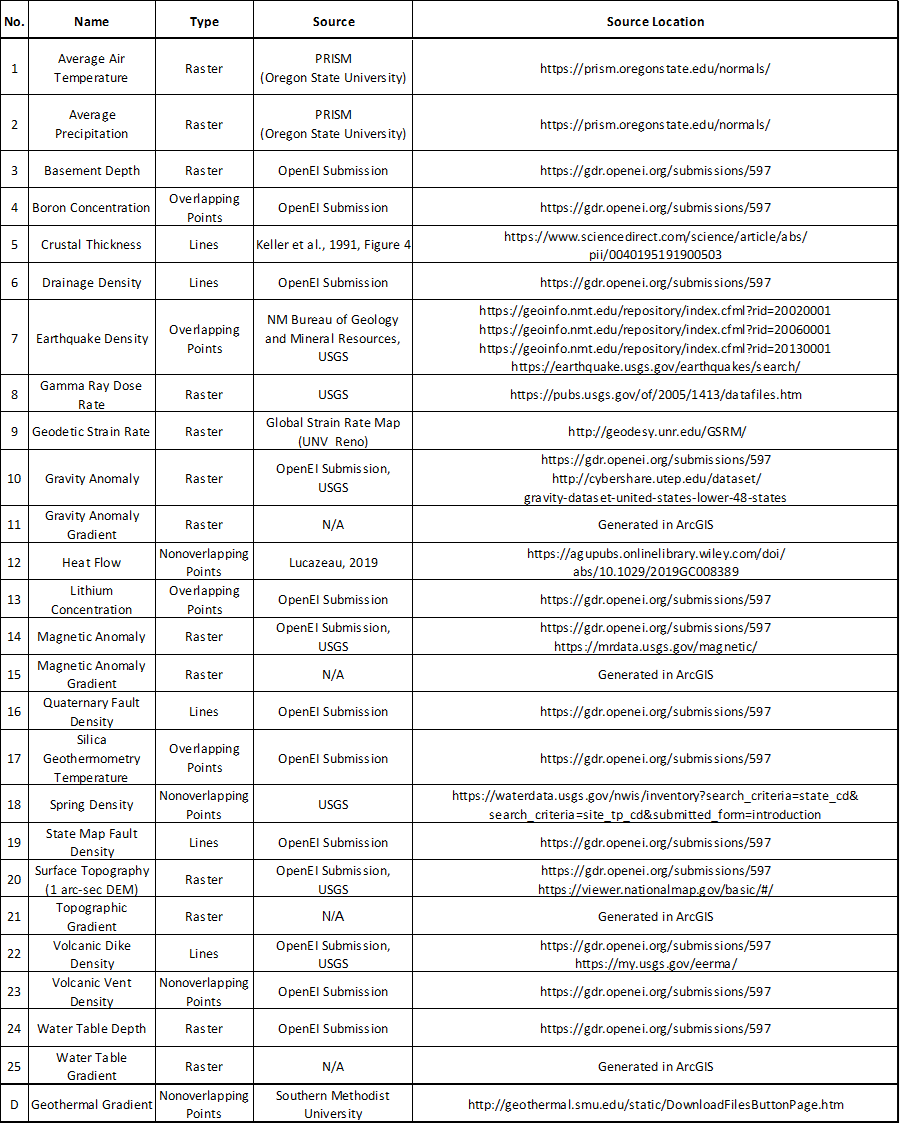
\includegraphics[width=\textwidth]{Table-Features.png}
\caption[Southwestern New Mexico features list]{List of data sets included in this analysis. Data type, source, and source location are noted. Suggested feature-sensitive risk elements include temperature/heat (T), fluids (F), and structure/permeability (P). Numbered features are treated as predictor variables. 'D' indicates the "dependent" or response variable.}
\label{tab:features}
\end{table}

As discussed in Section \ref{ch2:sysfund}, viable geothermal systems require permeability, heat, fluids, seal, and recharge. Following the more simplified PFA risk elements of \citet{bielicki_hydrogeolgic_2015}, an explorationist will want to identify where heat, permeability, and fluids together define a favorable setting for a geothermal prospect. The chosen feature inputs collectively address all three elements, as noted in Table \ref{tab:features}. Rather than defining a response variable that describes a total favorability score, this thesis focuses on a proof of concept predictive workflow for a physically-measurable quantity associated with the heat risk element: geothermal gradient. This choice was made because a) geothermal gradient provides a direct proxy for accessible heat content, b) gradient point data is available from suitable compilations of well measurements collected across the study area, and c) for EGS applications, the only risk element that must be naturally present is heat. Heat flow might be a reasonable alternative response variable, however point values for heat flow in the available well database were derived directly from geothermal gradient values. Geothermometer measurements also suggest resource temperatures, but the uncertainty in fluid pathways leading to the sample location means these values suffer from less spatial and depth certainty than geothermal gradient.

Regarding the remaining two risk elements: measurements of permeability (i.e., from downhole logs or core analysis) or fluids (e.g., flow rate from well tests) could be separately predicted using the same methods described in this study. A final favorability score, which is less straight-forward to calibrate for model validation and verification then geothermal gradient, could potentially be derived from the combined predictions of heat, permeability, and fluid presence as done in PFA risk assessments. This suggestion is outside of the scope of this thesis and thus appears in the list of future work opportunities \textbf{(see Chapter 9)}.

\section{Data Preparation}

In order to experiment with a variety of machine learning methods, all input data sets first need to be transformed into fully-complete \acrlong{gis} (\acrshort{gis}) layers such that any point on the map of the study area has a corresponding set of 25 predictor values. Steps taken to condition, process, and otherwise prepare each layer are outlined later in this chapter. As a preface, the following section reviews several fundamental concepts and algorithms utilized in the preparation of the data layers.

\subsection{Fundamentals}

\subsubsection{Extents}

The data sets imported into ArcGIS or Python scripts for feature preparation required cropping, gridding, or, less frequently, extrapolation to match each other in coverage of the southwest New Mexico study area. Two polygons were used for this purpose:

\begin{itemize}
\item \textbf{Regional Polygon}: this is a simple rectangular polygon capturing the broader southwestern NM region, defined by the following corner points in $^\circ$N Latitude and $^\circ$E Longitude: \\ (-31.3, -109.1), (31.3, -105.9), (35.4, -105.9), (31.3, -109.1)
\item \textbf{\acrlong{aoi} (\acrshort{aoi})}: this polygon appears in most map figures in this thesis and is the perimeter of a nine-county block in Southwest New Mexico that includes Cibola, Valencia, Catron, Socorro, Grant, Sierra, Luna, Dona Ana, and Hidalgo counties.
\end{itemize}

\subsubsection{Subsampling}\label{ssn:fishnet}

Machine learning models generally treat data as a matrix of observations. The concept of a geospatial dataframe follows this paradigm, where each row represents a discrete location specified in latitude and longitude columns, and all other columns contain feature values for that location. Since the area outlined by the study AOI covers 97,469 km$^2$, and each location is described by 25 features and 2 map coordinates, the matrix of the study area at 1 km$^2$ resolution would be of size 2,631,663 values. However, exploration typically does not require this level of granularity. Also, the time complexity of many machine learning methods grows at a non-linear rate with data size, e.g., the decision tree model discussed in Section \ref{ch5:decision_trees} has O(m\,n\,log$_{2}$n) complexity, where n is the number of observations and m is the number of features \citep{sani_computational_2018}. As such, a coarser resolution of $0.025^\circ$ ($\sim$2.5 km on average across the AOI) was selected as a manageable subsampling interval for this study. The ArcGIS \textit{Create Fishnet} tool generated a $0.025^\circ$ x $0.025^\circ$ mesh that, when constrained to the AOI polygon, consists of 15,137 point locations (Figure \ref{fig:fishnet}). Data preparation steps use this fishnet point set where noted in Section \ref{ch3:layers}, and final model predictions are made on these points to allow for direct comparison between different model results. 

\begin{figure}[htp]
\centering
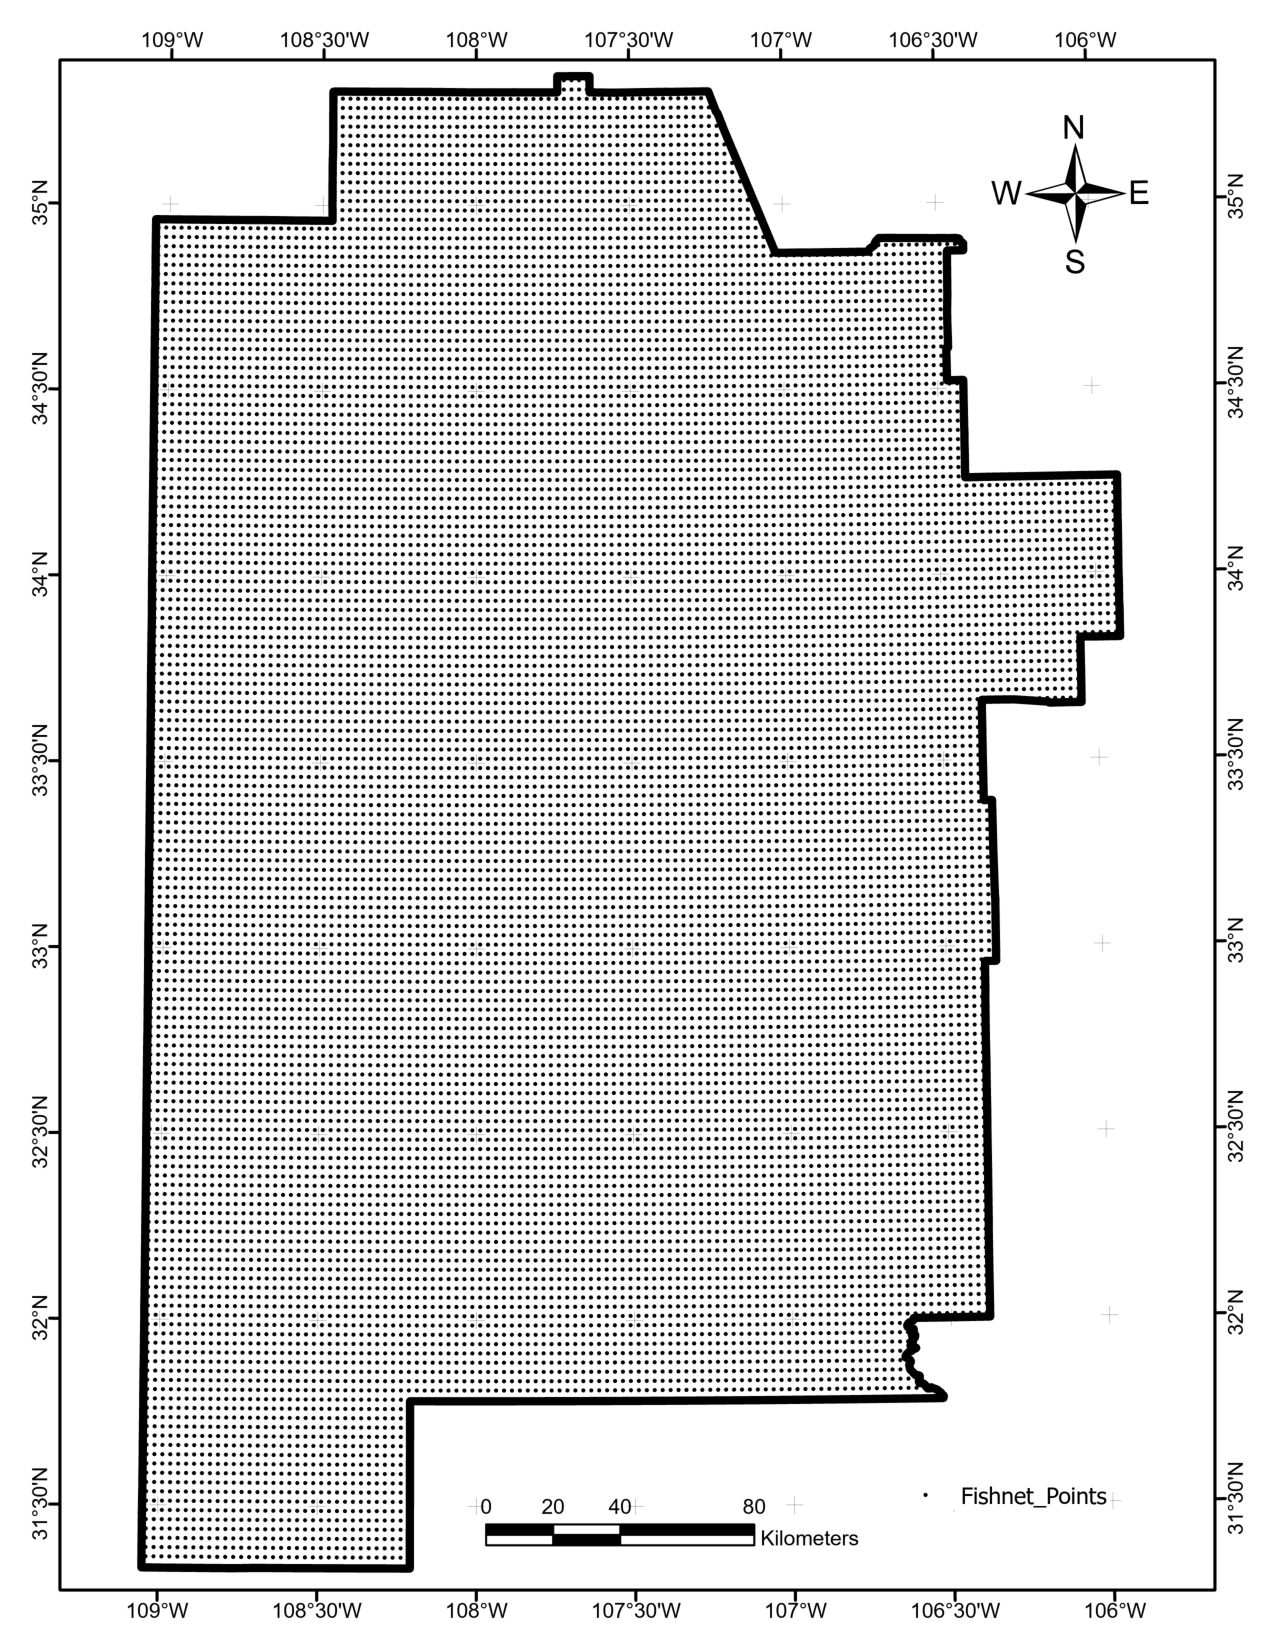
\includegraphics[scale=.50]{templates/images/Figure-Fishnet.pdf}
\caption[Fishnet point mesh]{Fishnet of points spaced $0.025^\circ$ apart in latitude and longitude.} 
\label{fig:fishnet}
\end{figure}

\subsubsection{Density Estimation}

One technique for converting a discrete set of points into a continuous field of values uses the concept of point density. The \acrlong{kde} (\acrshort{kde}) method fits a smooth function (kernel) to each point with the constraint that the volume under a kernel curve is 1.0. Density values assigned to cells of a gridded surface or raster image represent the sum over the curves crossing those cells. The kernel density tool can provide an estimate of density anywhere within the AOI, but it requires a kernel radius that sets the distance over which a point influences the density value. If left undefined, ArcGIS defaults to an optimal radius value based on a bandwidth formula \citep{esri_how_2021-3}. ArcGIS uses Silverman quartic kernels \citep{esri_how_2021-3,silverman_density_1986} as the functional basis in the \textit{Kernel Density} operation.

Polyline data can also be fit with smooth curves using the same density concept. The maximum value of the elongate curve follows the trace of the polyline, and the curve decays in value away from the line over a distance determined by the radius, which defaults to the bandwidth estimate. One difference for line density is the volume under the curve scales with line length. For more details on the ArcGIS implementation, refer to the \textit{Density toolset} documentation on \textit{Kernel Density} \citep{esri_how_2021-3}.

\subsubsection{Surface Fitting}

A multitude of algorithms exist for the purpose of fitting a set of values with a surface, thereby providing a means for interpolating missing values. Methods used in this thesis include the following four operations:

\begin{itemize}
\item{\textbf{Splines}}\label{ch3:splines} - Spline functions have a well-defined mathematical formulation that minimizes curvature while exactly fitting the input points. Regularized splines add a third derivative term, controlled by a weight parameter, that enforces a higher degree of smoothness with the trade-off of some misfit of the input data. This is helpful if outliers in the input point set would otherwise distort the spline fit. For details on the ArcGIS implementation, refer to the \textit{Interpolation toolset} documentation on the \textit{Spline} function \citep{esri_how_2021-2}.
\item{\textbf{Topo to Raster}}\label{ch3:topo2r} - The \textit{Topo to Raster} operation creates surfaces that honor the input data, typically contour sets, while ensuring i) correct representation of abrupt morphological features like rivers and ridges and ii) connectedness of drainage patterns. Specifically, \textit{Topo to Raster} uses an iterative finite difference method and an algorithm to remove sink points not supported by the input data, assuming natural sinks are rare and erroneous features in an interpolated surface. For details on the ArcGIS implementation, refer to the \textit{Interpolation toolset} documentation on the \textit{Topo to Raster} function \citep{esri_how_2021-1}.
\item{\textbf{Ordinary Kriging}}\label{ch3:kriging} - Kriging methods are geostatistical algorithms that take the correlation distance and directional bias into account when creating a surface. The two tasks involved in kriging include first estimating the functions that characterize these spatial relationships, then using these functions to generate predictions for interpolation (and extrapolation). For the first task, semivariograms are calculated by binning the semivariance of points based their distance from each other, then fitting a model curve (e.g. linear, spherical, exponential) to these values. Semivariograms can be anisotropic, meaning they can vary with direction. The second task uses the semivariogram to define a weighted average of the input data when estimating new values. For more details on the ArcGIS implementation, refer to the \textit{Interpolation toolset} documentation on the \textit{Kriging} function \citep{esri_how_2021}.
\item{\textbf{\acrlong{ebk} (\acrshort{ebk})}}\label{ch3:ebk} - The EBK algorithm extends ordinary kriging by automating parameter selections and accounting for uncertainty in semivariogram estimation. Ordinary kriging generates a single variogram and treats it as ground truth while EBK generates an ensemble of semivariograms that can be used for greater accuracy in estimating standard errors. As a computationally heavy methodology, EBK takes much longer to apply than ordinary kriging or other methods. For more details on the ArcGIS implementation, refer to the documentation on the \textit{Empirical Bayes Kriging} function \citep{esri_what_2021}.

\end{itemize}

\subsection{Data Layers}\label{ch3:layers}

\subsubsection{Average Air Temperature}

The University of Oregon PRISM Climate Group maintains regularly-updated spatial data sets of climate-related observations, including 30-year normals describing average annual conditions \citep{daly_physiographically_2008, prism_prism_2021}. The 800 m resolution average air temperature grid was downloaded and imported into ArcGIS, then cropped using the Regional Polygon (Figure \ref{fig:feat_airtemp}). This layer required no further processing.

\begin{figure}[!htp]
\centering
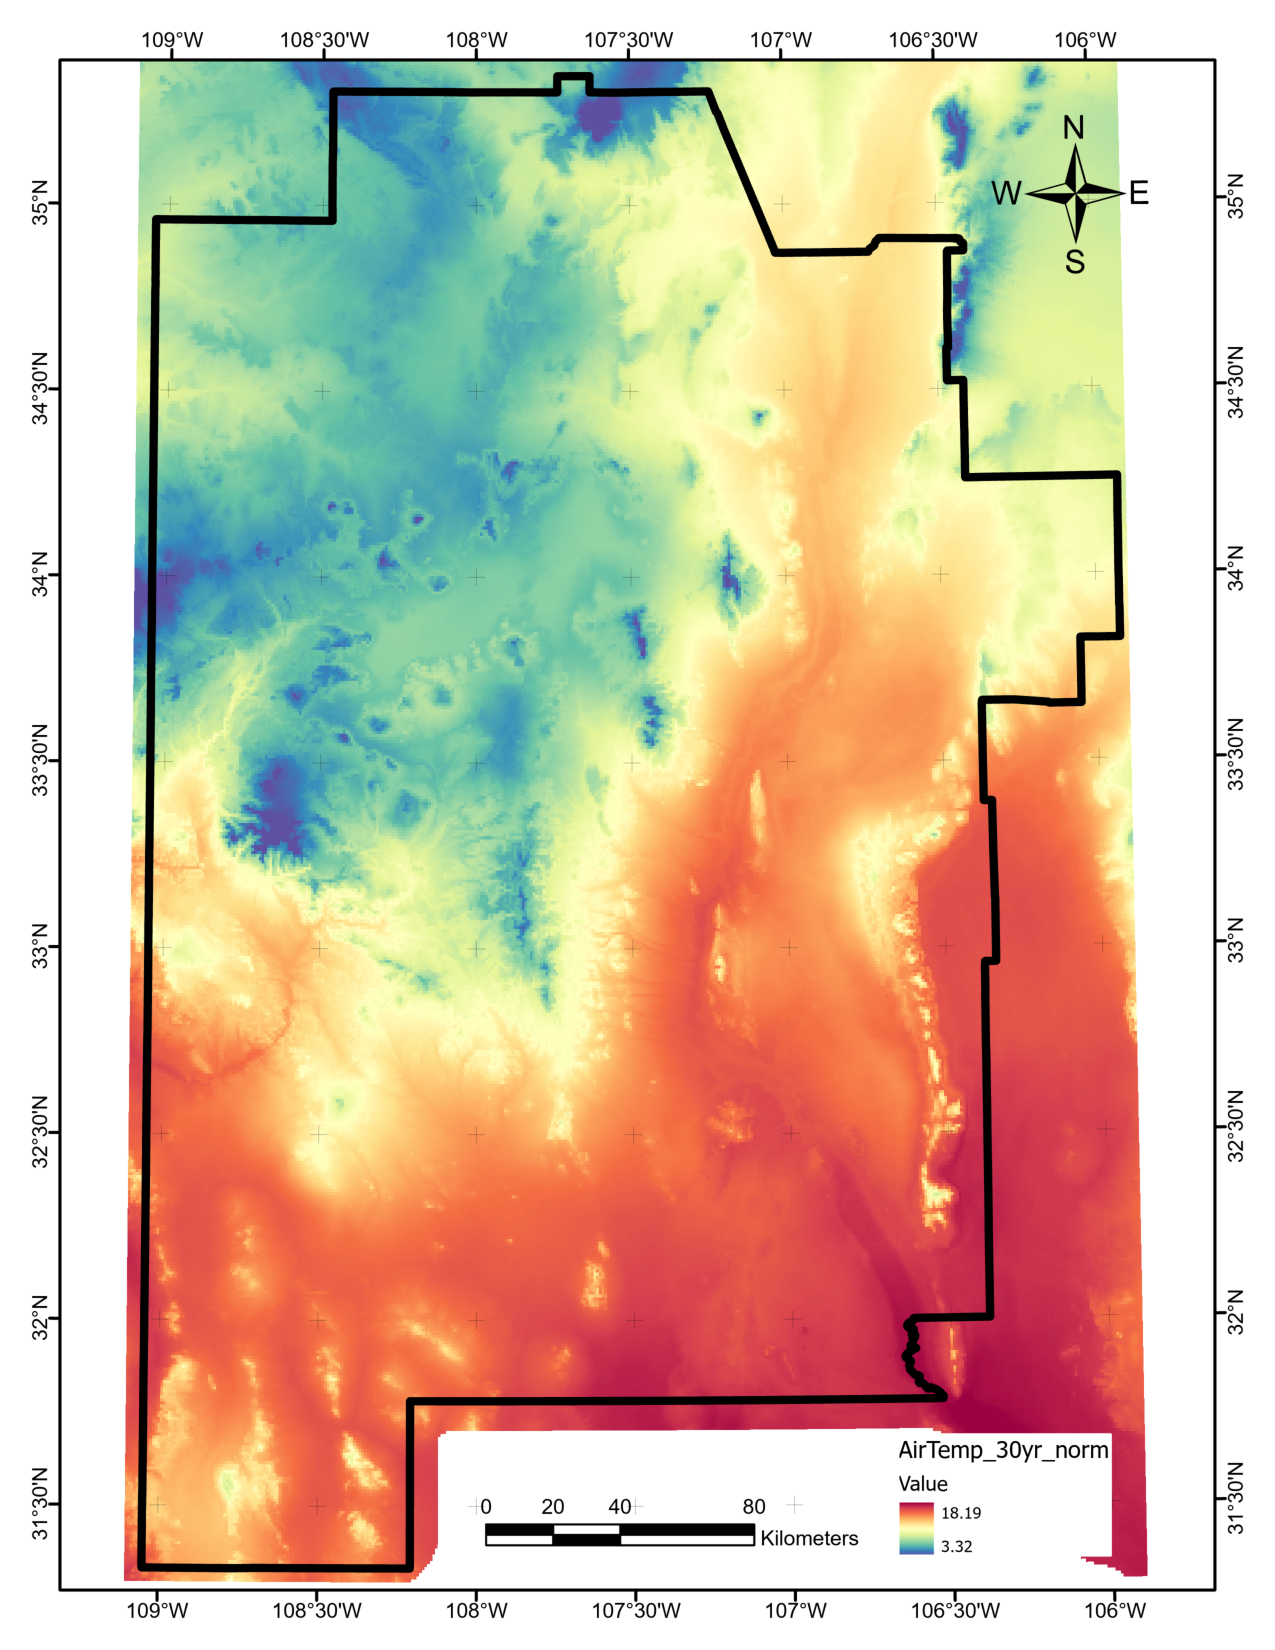
\includegraphics[scale=.50]{templates/images/Figure-AvgAirTemp.pdf}
\caption[Average air temperature data layer]{Average air temperature data layer. Units are in $^\circ$C. Data retrieved from the PRISM website \protect\citep{prism_prism_2021}.}
\label{fig:feat_airtemp}
\end{figure}

\subsubsection{Average Precipitation}

The University of Oregon PRISM Climate Group also compiles 30-year normals for precipitation \citep{daly_physiographically_2008, prism_prism_2021}. The 800 m resolution average precipitation grid was downloaded and imported into ArcGIS, then cropped to the Regional Polygon boundary (Figure \ref{fig:feat_precip}). This layer required no further processing.

\begin{figure}[!htp]
\centering
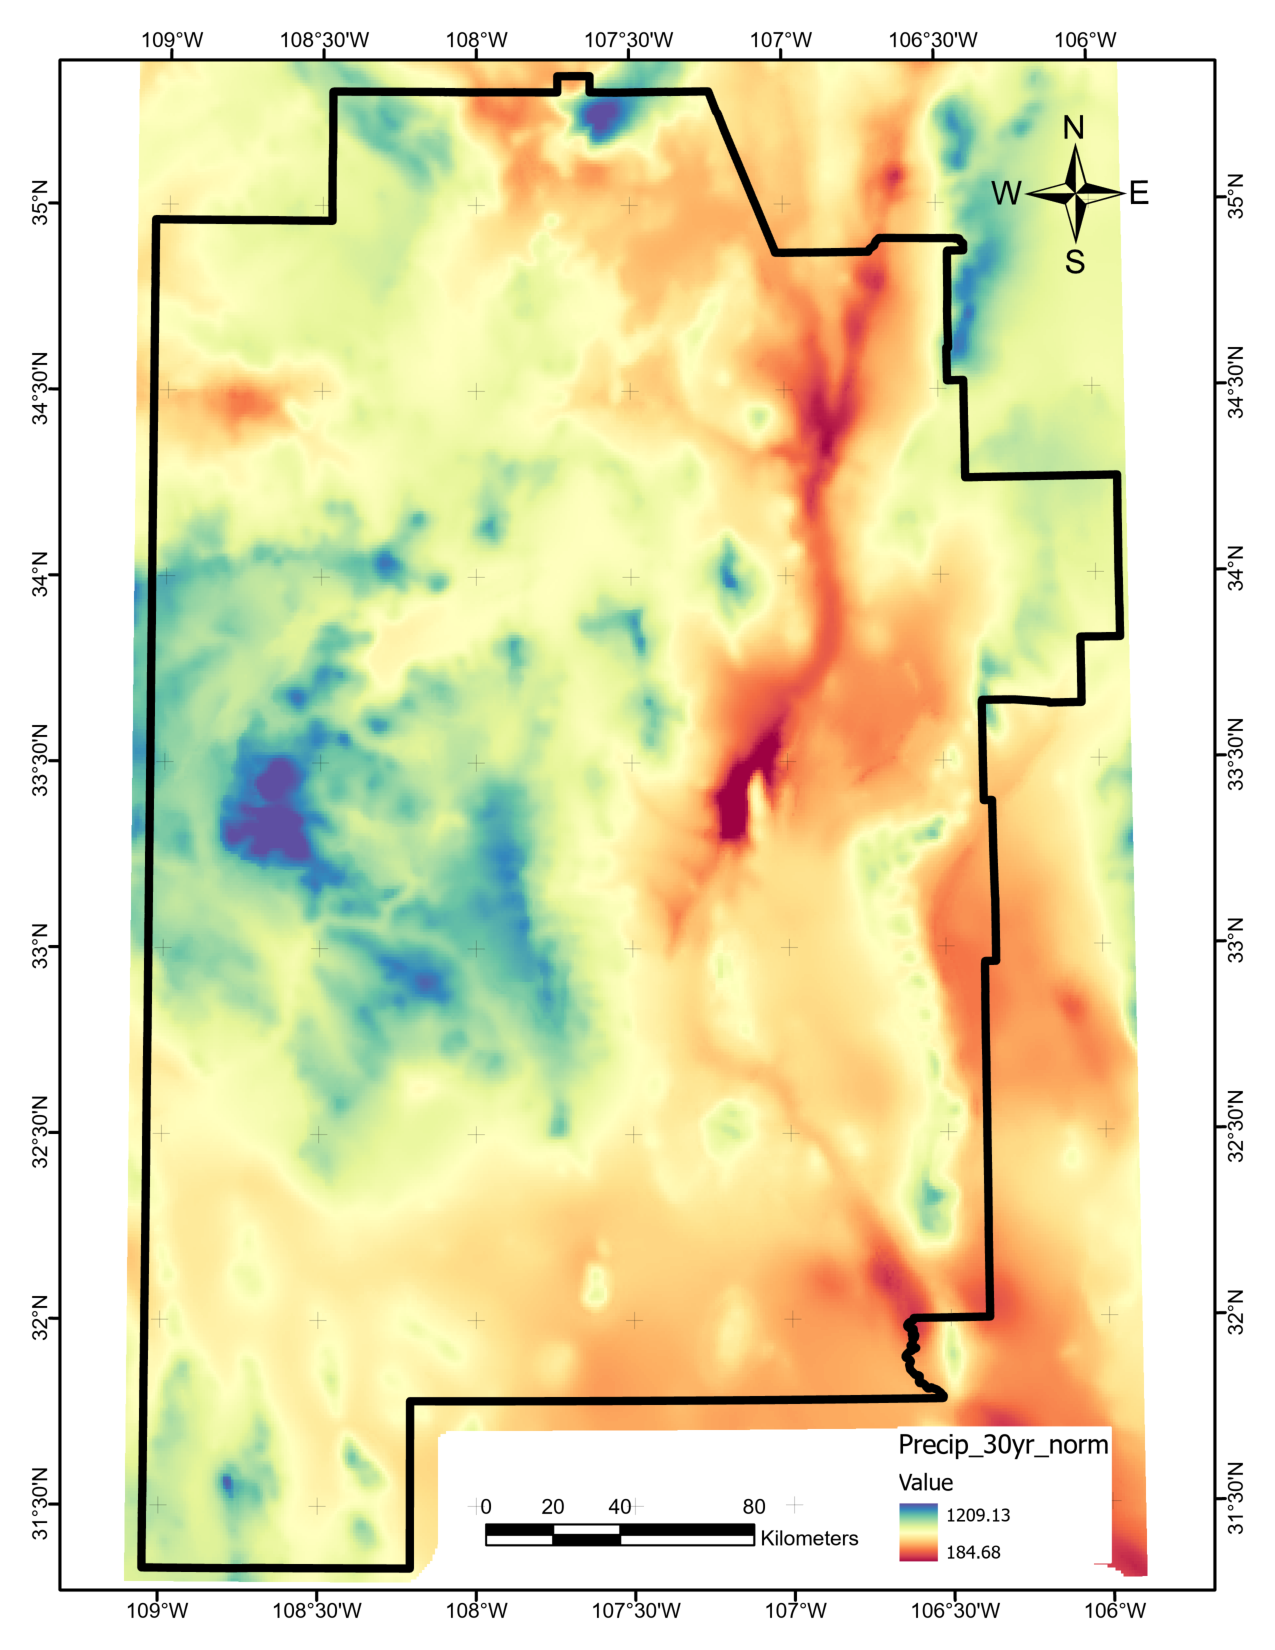
\includegraphics[scale=.50]{templates/images/Figure-AvgPrecip.pdf}
\caption[Average precipitation data layer]{Average precipitation data layer in 800 m resolution. Units are in millimeters. Data retrieved from the PRISM website \protect\citep{prism_prism_2021}.}
\label{fig:feat_precip}
\end{figure}

\subsubsection{Basement Depth}

Following the procedure of \citet{pepin_new_2018}, the basement elevation raster generated by \citet{bielicki_hydrogeolgic_2015} was downloaded, imported into ArcGIS, and processed to calculate depth to basement. Specifically, a unit conversion from feet to meters was applied to the basement elevation surface. Then, values were extracted on the point fishnet (see \ref{ssn:fishnet}), which highlighted missing data patches in the data. The ArcGIS \textit{Kriging} function interpolated values across these patches using a spherical semivariogram, auto-determined lag size of 0.097, and a variable search radius with a 4-point requirement. Basement depths were then calculated by subtracting the interpolated elevation layer from the Surface Topography (DEM) layer. However, the higher resolution of the DEM layer caused an imprint of detailed surface morphologies to appear on the calculated basement depth layer. To correct for this, the DEM layer was low-pass filtered using the ArcGIS \textit{Filter} method, which averages a 3x3 neighborhood around each point in the data set. The final basement elevation layer (Figure \ref{fig:feat_basementdepth}) was generated from the difference between the filtered DEM and the interpolated basement elevation layers.

\begin{figure}[!htp]
\centering
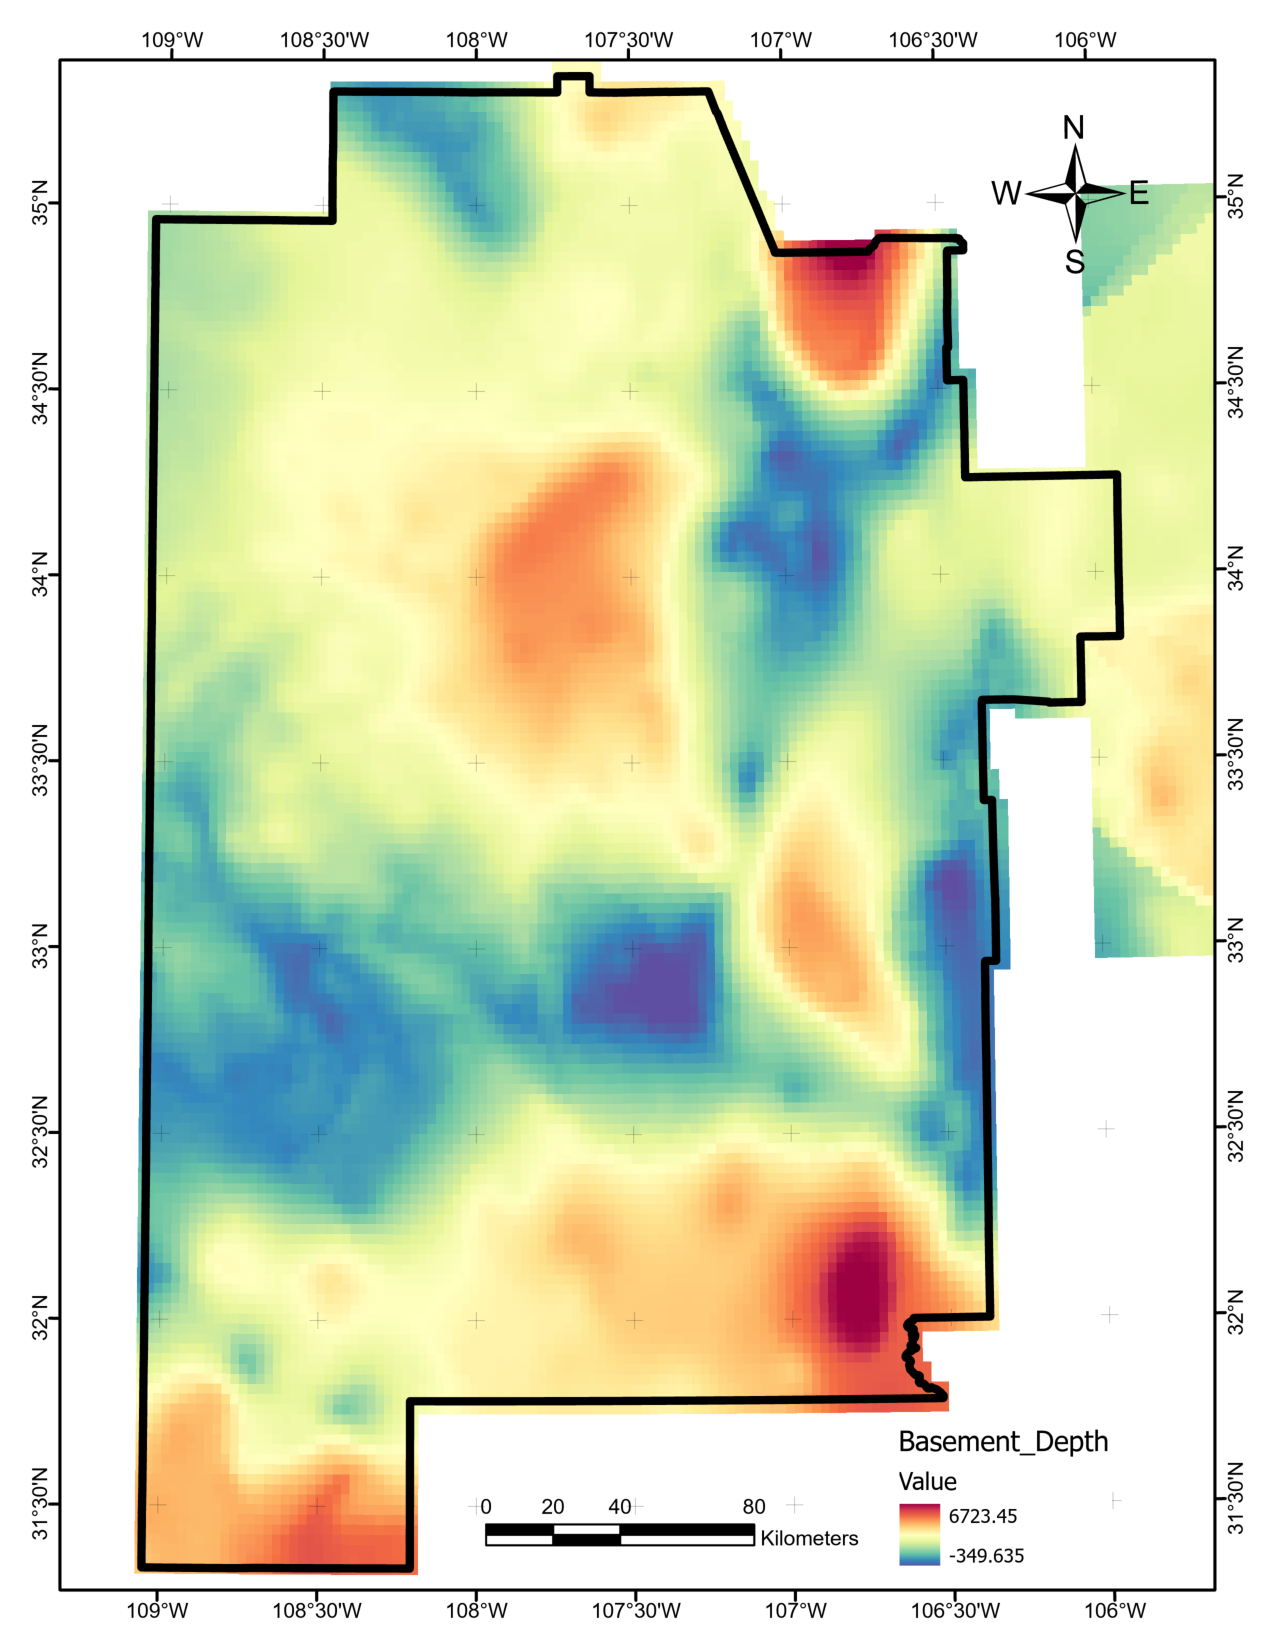
\includegraphics[scale=.50]{templates/images/Figure-BasementDepth.pdf}
\caption[Basement depth data layer]{Basement depth data layer. Units are in meters. Layer based on basement elevation raster from \protect\citep{bielicki_hydrogeolgic_2015}.}
\label{fig:feat_basementdepth}
\end{figure}

\subsubsection{Boron Concentration}

Measurements of boron concentration were originally assembled by \citet{bielicki_hydrogeolgic_2015} from USGS records, student dissertations, and other sources. These data were downloaded from the OpenEI submission \citep{kelley_geothermal_2015} and merged together using ArcGIS and Python to create a single dataframe of 5,686 measurements, all within the broader Regional Polygon bounds to avoid surface creation edge effects within the tighter AOI. The inconsistent spatial distribution of the data, and sometimes significant variation among overlapping values from different measurement years, created a unique challenge for making a representative GIS layer to use for analysis. An initial attempt to fit and interpolate the data using tuned Gaussian Process models created feature layers with too much local structure and little character away from the input data points. The ArcGIS \textit{Empirical Bayes Kriging} routine was selected instead due to its ability to manage coincident data and high accuracy with smaller data sets compared to ordinary kriging methods. For the final layer, EBK was applied with the empirical data transformation type, a maximum of 100 points in each local model, 100 simulated semivariograms with k-Bessel model type, and a standard circular search neighborhood with a radius of 1.1957 (auto-determined), minimum of 10 neighbors, and maximum of 15 neighbors. The output grid cell size was set to 0.01 degrees. Of important note: the calculation option to include all coincident data was selected, so all overlapping measurements were considered in generating the final layer (Figure \ref{fig:feat_boron}).

\begin{figure}[!htp]
\centering
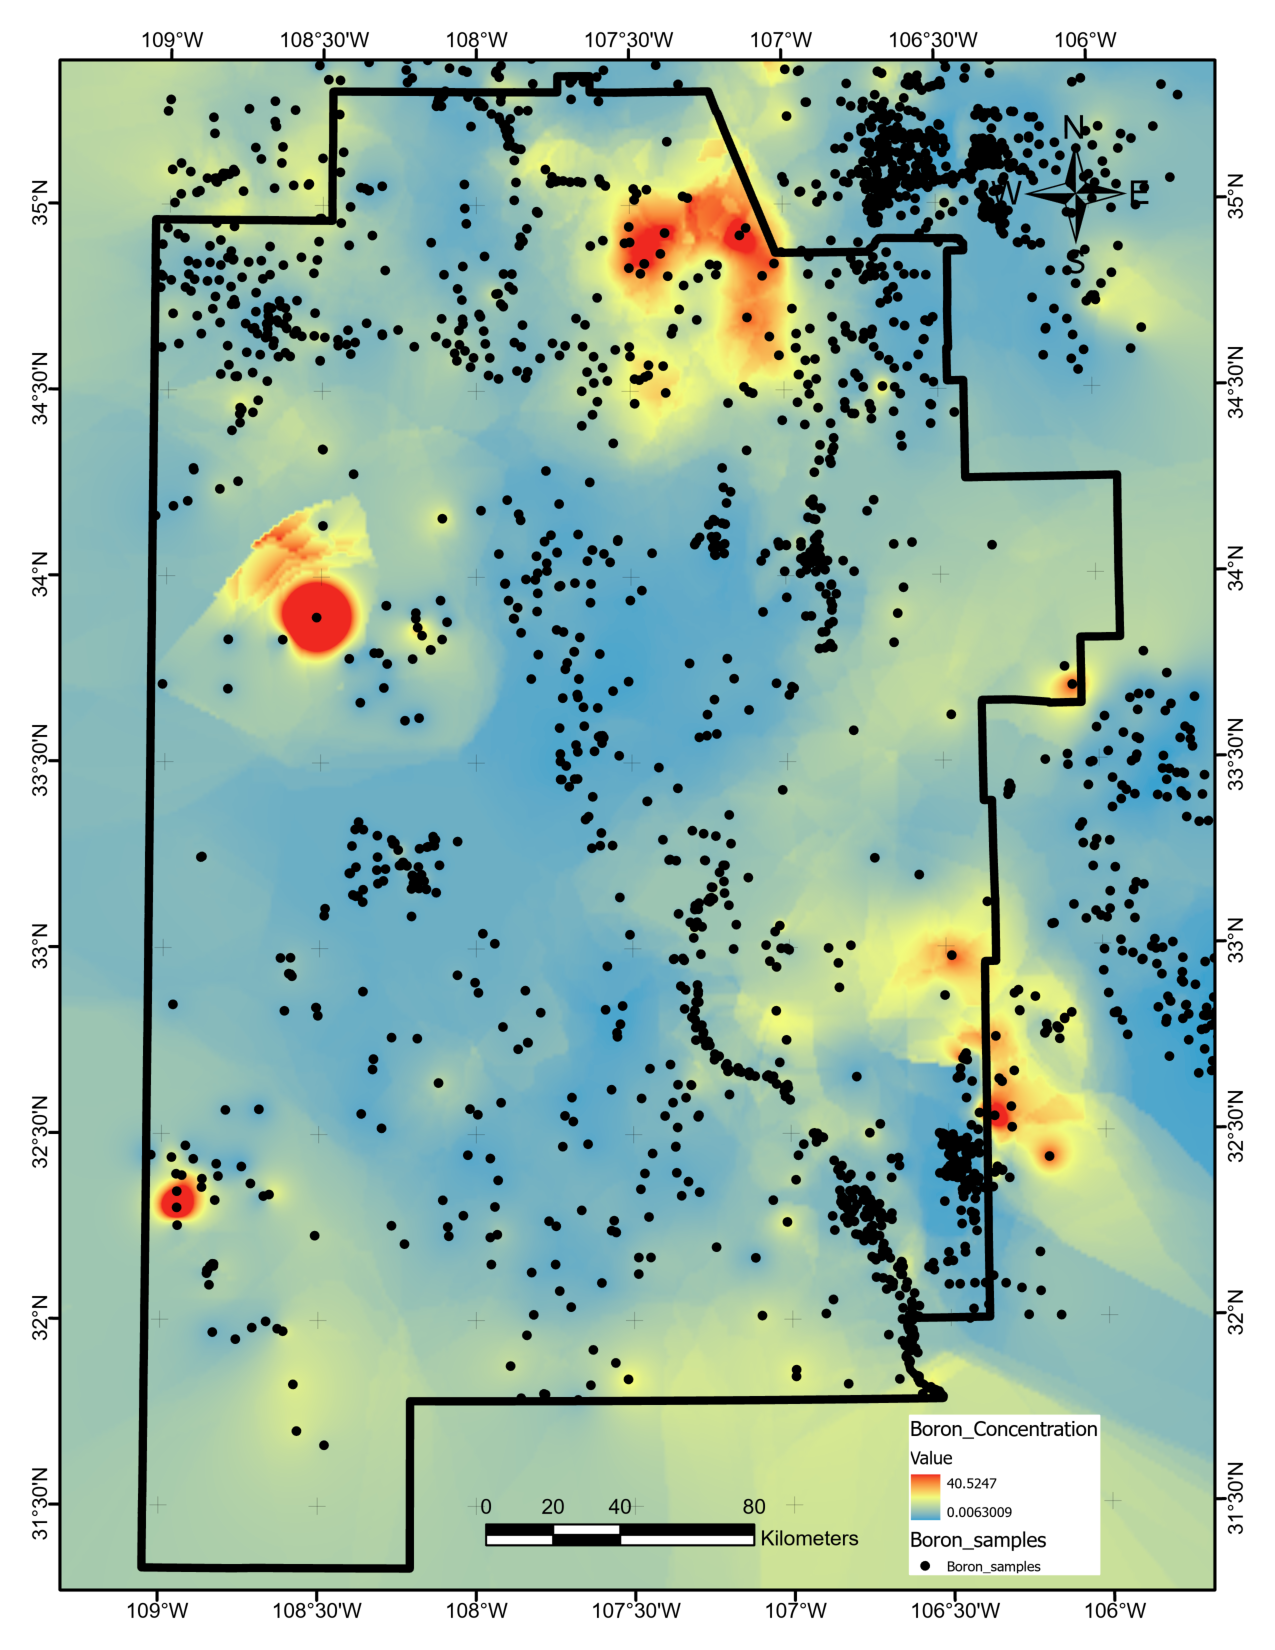
\includegraphics[scale=.50]{templates/images/Figure-Boron.pdf}
\caption[Boron concentration data layer]{Boron concentration data layer. Units are in ppm or mg/L. Black dots indicate sample locations in complete data set from \protect\citep{bielicki_hydrogeolgic_2015}.}
\label{fig:feat_boron}
\end{figure}

\subsubsection{Crustal Thickness}

In the absence of a more recent seismic study constraining variations in crustal thickness across the study area, the regional map published by \citet{keller_comparative_1991} was used to construct the crustal thickness feature layer. Similar to the procedure described in \citep{pepin_new_2018}, the Keller map was georeferenced in ArcGIS, and thickness contours were manually digitized as polylines. These polylines continued slightly beyond the AOI boundary to ensure proper constraints for surface creation without artifacts near the AOI edges. The ArcGIS function \textit{Feature to 3D by Attribute} converted the polylines into 3D contours, and \textit{Topo to Raster} interpolated the contours into a continuous final grid (Figure \ref{fig:feat_crust}). Since the Keller map was derived from low-resolution seismic lines from the 1960s-1980s, the result is a very low frequency approximation for crustal thickness variations associated with the CP and RGR provinces. As such, a slightly larger cell size of 0.025 degrees was used than for other layers. Additional parameter choices included: margin in the cells of 20, smallest z value for interpolation of 25, largest z value for the interpolation of 55, drainage enforcement, and maximum iterations of 20.

\begin{figure}[!htp]
\centering
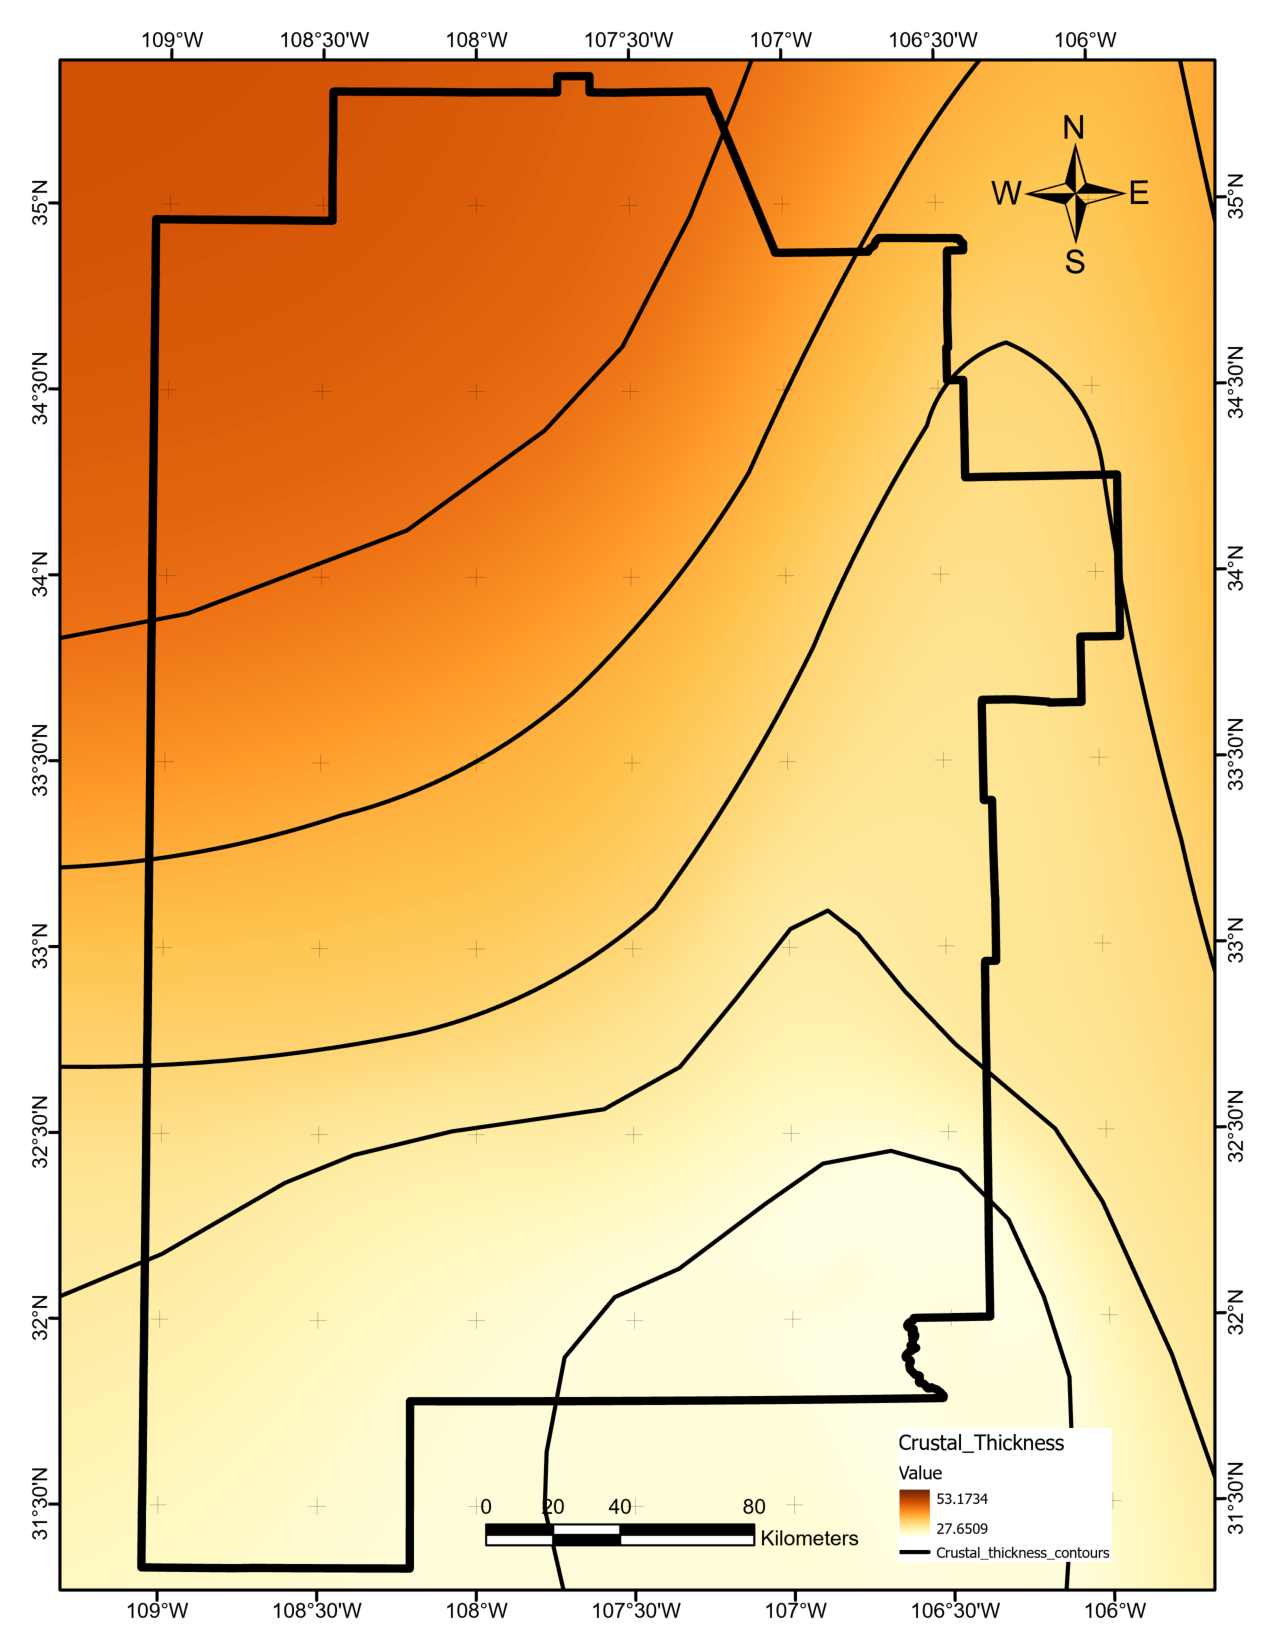
\includegraphics[scale=.50]{templates/images/Figure-CrustalThickness.pdf}
\caption[Crustal thickness data layer]{Crustal thickness data layer. Units are in kilometers. Black lines trace the contours digitized from \protect\citep{keller_comparative_1991}.}
\label{fig:feat_crust}
\end{figure}

\subsubsection{Drainage Density}

Drainage polyline data comes from the \citet{bielicki_hydrogeolgic_2015} PFA OpenEI submission \citep{kelley_geothermal_2015}. The data were downloaded and imported into ArcGIS, then compared to the DEM layer for quality control. A couple of methods were attempted in order to transform this feature into a continuous-valued layer with full map coverage. First, the polylines were converted to points with 500 m sampling. This point set was loaded into a Python script, which used a grid search routine to determine the best radius for a Gaussian KDE routine available in the scikit-learn package \citep{pedregosa_scikit-learn_2011}. Ten-fold cross validation was employed, which splits the data into 10 subsets and interchangeably trains on 9, tests on one to get an average performance score. Based on a calculation of the negative log likelihood, the best radius was found to be 45,600 m. However, when the kernel density operation is applied to the data with this radius, the map shows a central blob of high density, which falls off toward the sides of the survey. With such a large kernel radius, edge effects come into play since no drainage polylines were available outside of the AOI boundary. Furthermore, the conversion of line data to points for this method disregards the spatial relationships of the connected line data. The ArcGIS \textit{Kernel Density} operation, which handles line data and auto-determines the kernel radius, produced a layer with more reasonable density relationships based on visual inspection. The final drainage density layer (Figure \ref{fig:feat_drainage}) used an output cell size of 0.0025 degrees and auto-determined search radius of 0.272.

\begin{figure}[!htp]
\centering
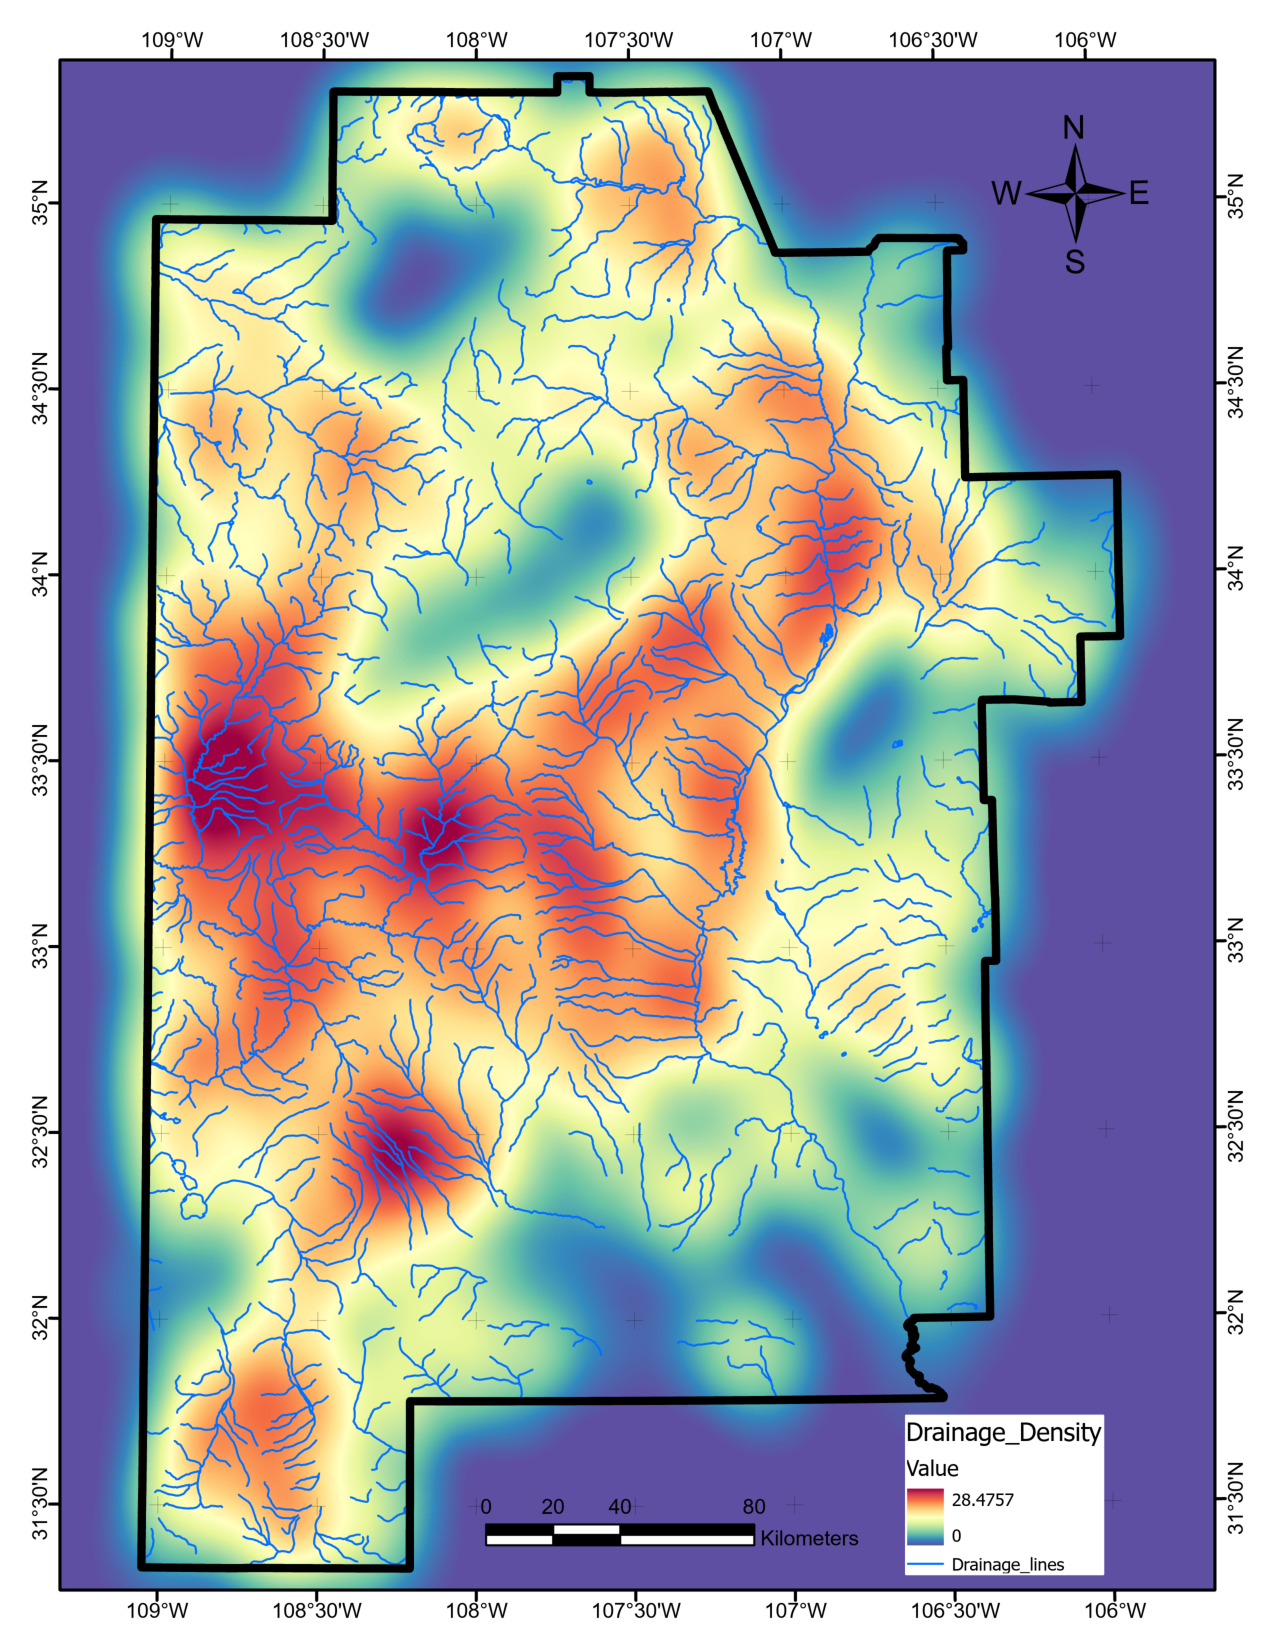
\includegraphics[scale=.50]{templates/images/Figure-DrainageDensity.pdf}
\caption[Drainage density data layer]{Drainage density data layer. Units are in degrees/degrees$^2$. Blue lines show the drainage polyline data set from \protect\citep{bielicki_hydrogeolgic_2015}.}
\label{fig:feat_drainage}
\end{figure}

\subsubsection{Earthquake Density}
%%\captionsetup[figure]{skip=0pt}
\begin{wrapfigure}{R}{0.5\linewidth}
\centering
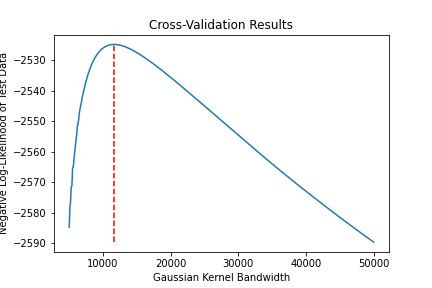
\includegraphics[scale=0.6]{templates/images/Figure-Earthquakes_kde_gridsearchcv_result.png}
\singlespacing
\caption[Earthquake density parameter tuning]{Cross-validation results for earthquake KDE. Red dashed line indicates maximum negative log likelihood value identifying the best kernel radius.}
\label{fig:EQ_cv}
\end{wrapfigure}
Following the procedure outlined by \citet{pepin_new_2018}, an earthquake data set for southwest New Mexico was created by combining historical earthquake catalogs for 1869-1998 \citep{sanford_earthquake_2002}, 1999-2004 \citep{sanford_earthquake_2006}, and 2005-2009 \citep{pursley_earthquake_2013} with data pulled from the USGS Earthquake catalog \citep{usgs_earthquake_2021} through to January 2021. All events were combined into a single dataframe in Python, and event duplicates were removed. The final catalog, cropped to the Regional Polygon boundary, consists of 2,539 events spanning 1962-2020. This point set was loaded into a KDE Python script, which used a grid search to determine the best radius for the scikit-learn \textit{KernelDensity} routine \citep{pedregosa_scikit-learn_2011}. Ten-fold cross validation was employed, which splits the data into 10 subsets and then interchangeably trains on 9 and tests on one to get an average performance score. The maximum negative log likelihood indicates a best radius value of 11,600 m (Figure \ref{fig:EQ_cv}). 

KDE values calculated at each fishnet point location were loaded into ArcGIS, and the \textit{Kriging} function created a final surface for plotting purposes (Figure \ref{fig:feat_EQ_density}). \textit{Kriging} parameters included: spherical semivariogram model, lag size of 1e-6, variable search radius with 12-point requirement, and output cell size of 0.01.

\begin{figure}[!htp]
\centering
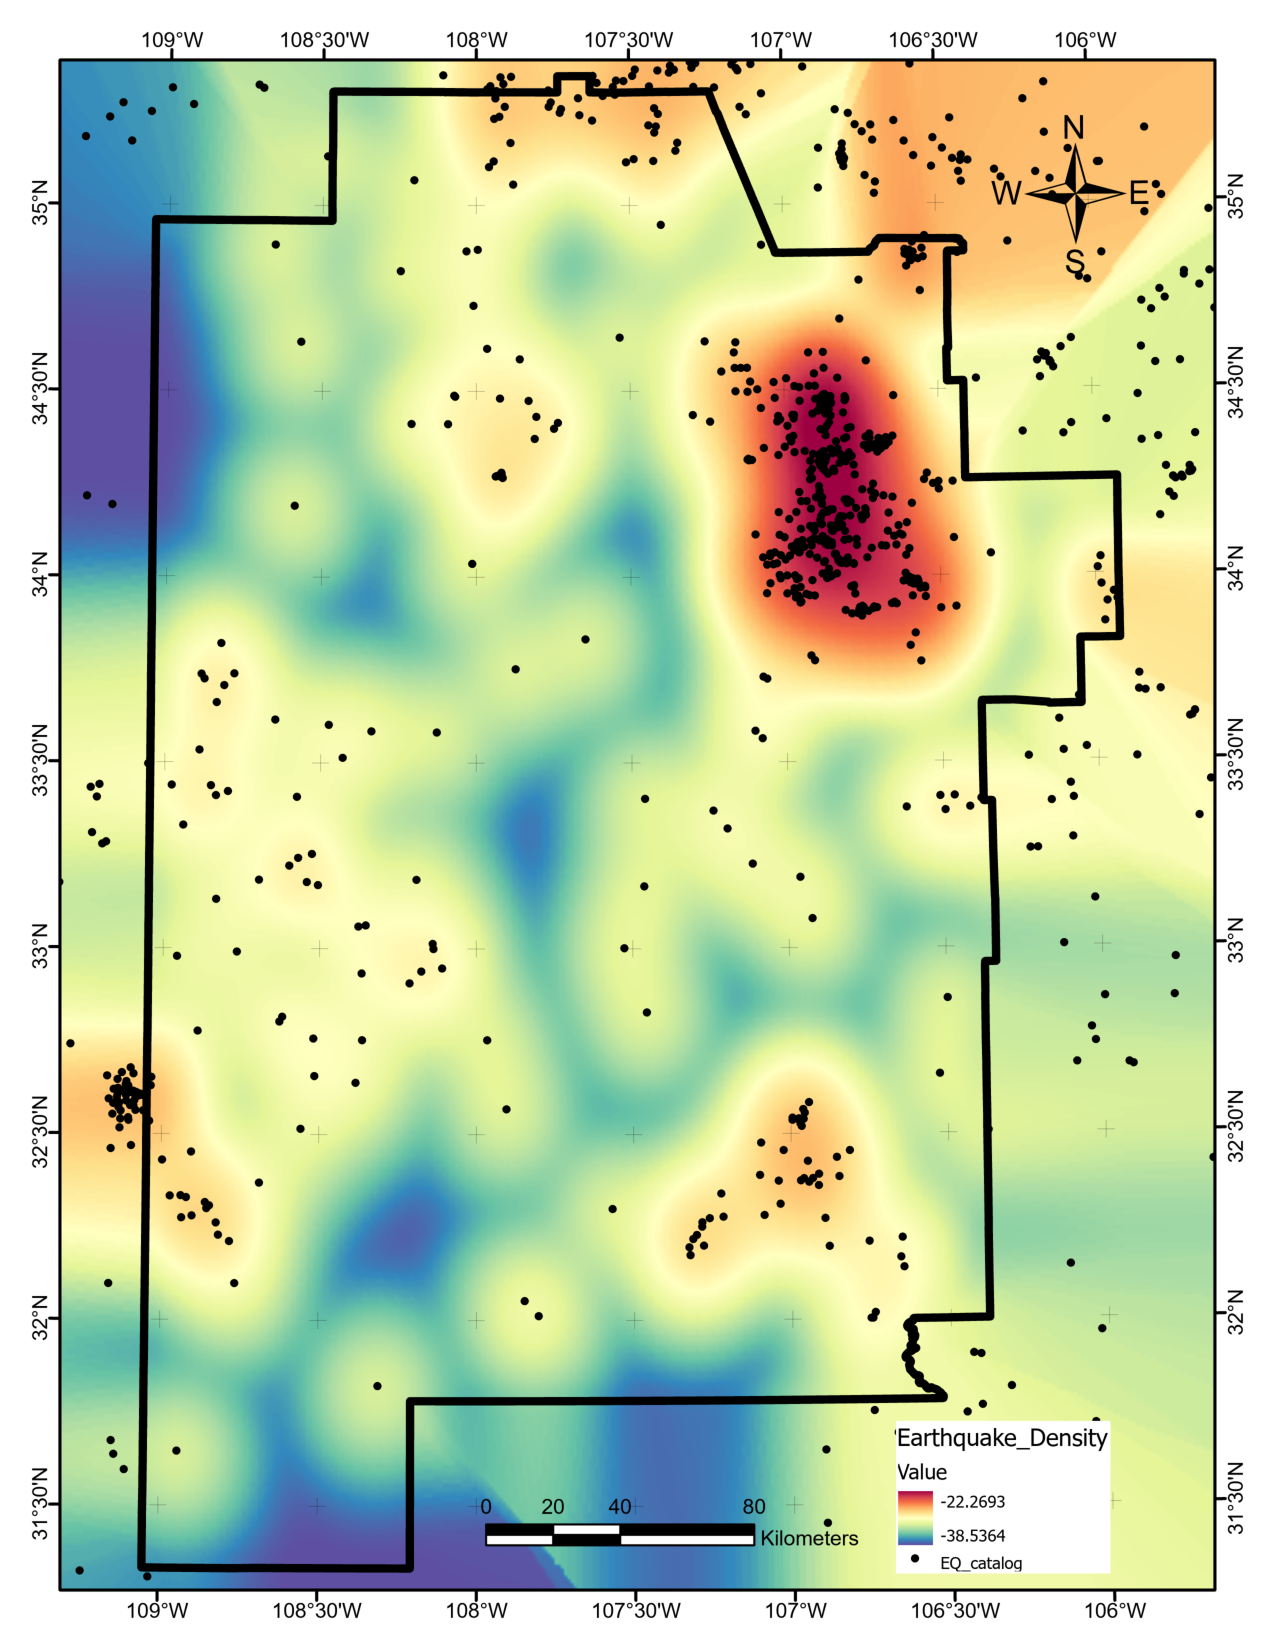
\includegraphics[scale=.50]{templates/images/Figure-EarthquakeDensity.pdf}
\caption[Earthquake density data layer]{Earthquake density data layer. Units are in log(points/km$^2$). Black dots indicate earthquake locations.}
\label{fig:feat_EQ_density}
\end{figure}

\subsubsection{Gamma Ray Dose Rate}

Aerial gamma ray surveys conducted across the United States in the late 1970-1980s allowed for the construction of Potassium concentration (K, in percent K), Uranium concentration (eU, in ppm), and Thorium concentration (eTh in ppm) maps, which tie back to mineralogy and hence are a proxy for stratigraphy. These measures collectively define the absorbed dose rate, which can be calculated from the following equation: $D = 13.2 K + 5.48 eU + 2.72 eTh$ \citep{duval_terrestrial_2005}.

The absorbed dose rate for West Central USA was downloaded from the USGS Open-File Report 2005-1413 website \citep{duval_terrestrial_2005}, loaded into ArcGIS, and cropped to the Regional Polygon bounds. A data gap in the vicinity of the White Sands Missile Range to the southeast of the study area necessitated layer interpolation using kriging. Grid values were extracted using the point fishnet, then passed through the ArcGIS \textit{Kriging} function to create the final layer (Figure \ref{fig:feat_gamma}) based on the following preferred parameters: spherical semivariogram model, auto-determined lag size of 0.097, and a variable search radius with a 4-point requirement.

\begin{figure}[!htp]
\centering
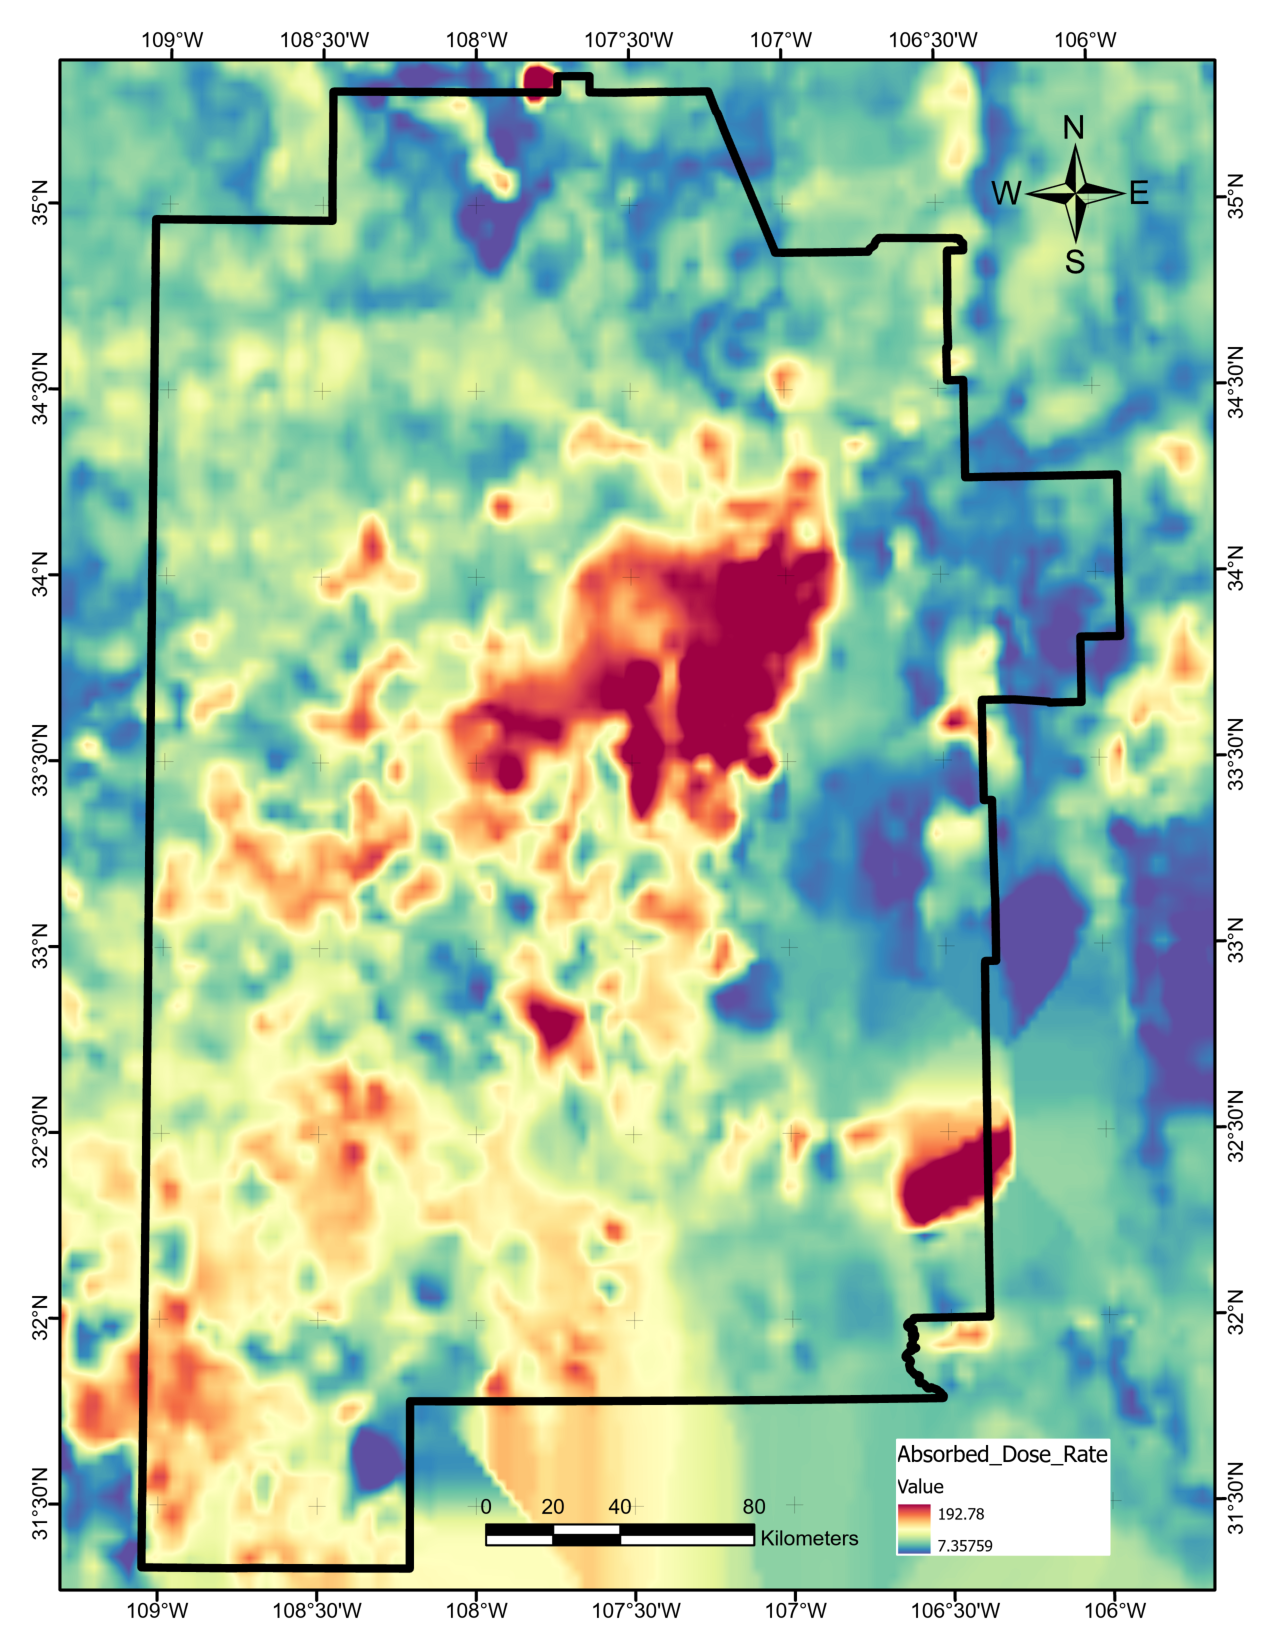
\includegraphics[scale=.50]{templates/images/Figure-AbsorbedDose.pdf}
\caption[Absorbed dose rate data layer]{Absorbed dose rate data layer. Units are in nanoGrays/hour (nGy/hr). Original data from USGS Open-File Report 2005-1413 \protect\citep{duval_terrestrial_2005}}.
\label{fig:feat_gamma}
\end{figure}

\subsubsection{Geodetic Strain Rate}

GPS stations worldwide record local movements in the Earth’s crust. These movements can highlight inflation or subsidence of the surface, fault motions, or plate tectonic activity. The spatial derivative of crustal velocities is termed the strain rate, which gives an indication of the accumulation of strain in an area. More concretely, it defines the speed with which the crust is deforming, and can be treated as a proxy for earthquake potential since slip occurs due to the accumulation of strain \citep{gem_strain_2014}. The Global Strain Rate Model (GSRM) v.2.1 provides a model for strain rate based on over 22,000 measurements from over 18,000 locations around the world \citep{kreemer_geodetic_2014}. The output of this model was downloaded from the University of Nevada Reno Geodetic Laboratory host site \citep{kreemer_global_2020}. GSRM describes elements of the full strain tensor at a $0.1^\circ$ resolution. The magnitude or second invariant of the strain tensor can combine these elements into a single value \citep{kreemer_geodetic_2014}:

\begin{equation}\label{eq:strainratemagnitude}
\left\lVert\dot{\epsilon}\right\rVert = \sqrt{\dot{\varepsilon}_{\phi\phi}^2+\dot{\varepsilon}_{\theta\theta}^2+2\dot{\varepsilon}_{\phi\theta}^2}
\end{equation}

Due to the size of the model file and complexity of this calculation, the data was first loaded into Python, cropped to the Regional Polygon bounds, and the strain rate magnitude was calculated for each point. These data were then loaded into ArcGIS and gridded using the \textit{Spline} function for a smooth interpolation of the coarser GSRM grid. The final layer (Figure \ref{fig:feat_strain}) was created using the following \textit{Spline} parameters: regularized type, weight of 0.1, 4-point requirement, and cell size of 0.025 degrees.

\begin{figure}[!htp]
\centering
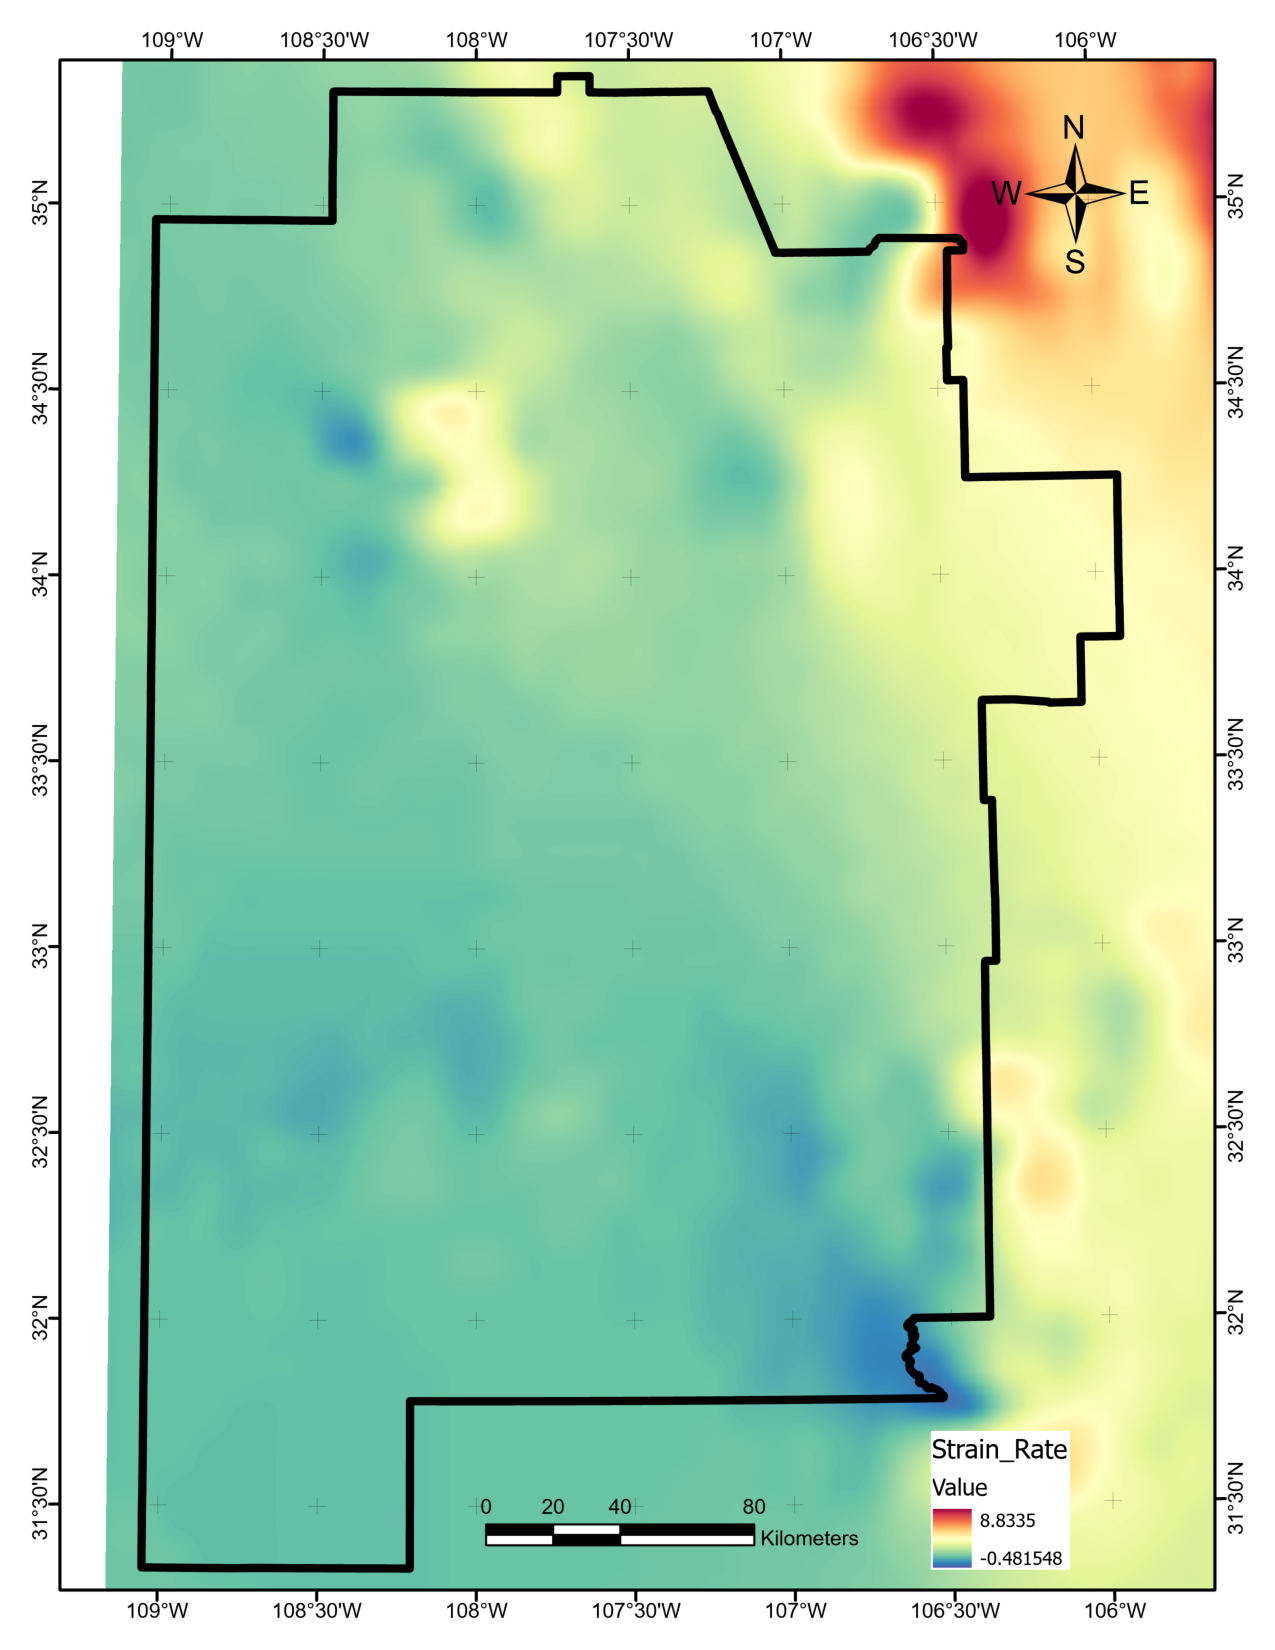
\includegraphics[scale=.50]{templates/images/Figure-StrainRate.pdf}
\caption[Geodetic strain rate data layer]{Geodetic strain rate data layer. Units are in $10^-9$m/(m*yr). Layer is based on data from \protect\citep{kreemer_geodetic_2014}}.
\label{fig:feat_strain}
\end{figure}

\subsubsection{Gravity Anomaly}

Terrain-corrected gravity anomaly data available from the University of Texas El Paso \citep{utep_gravity_2011} were used in both the PFA analysis \citep{bielicki_hydrogeolgic_2015} and cluster analysis \citep{pepin_new_2018} for southwest NM. The data layer from \citet{bielicki_hydrogeolgic_2015} was downloaded from their OpenEI submission \citep{kelley_geothermal_2015} and loaded into ArcGIS. This layer (Figure \ref{fig:feat_gravity}) required no further processing.

\begin{figure}[!htp]
\centering
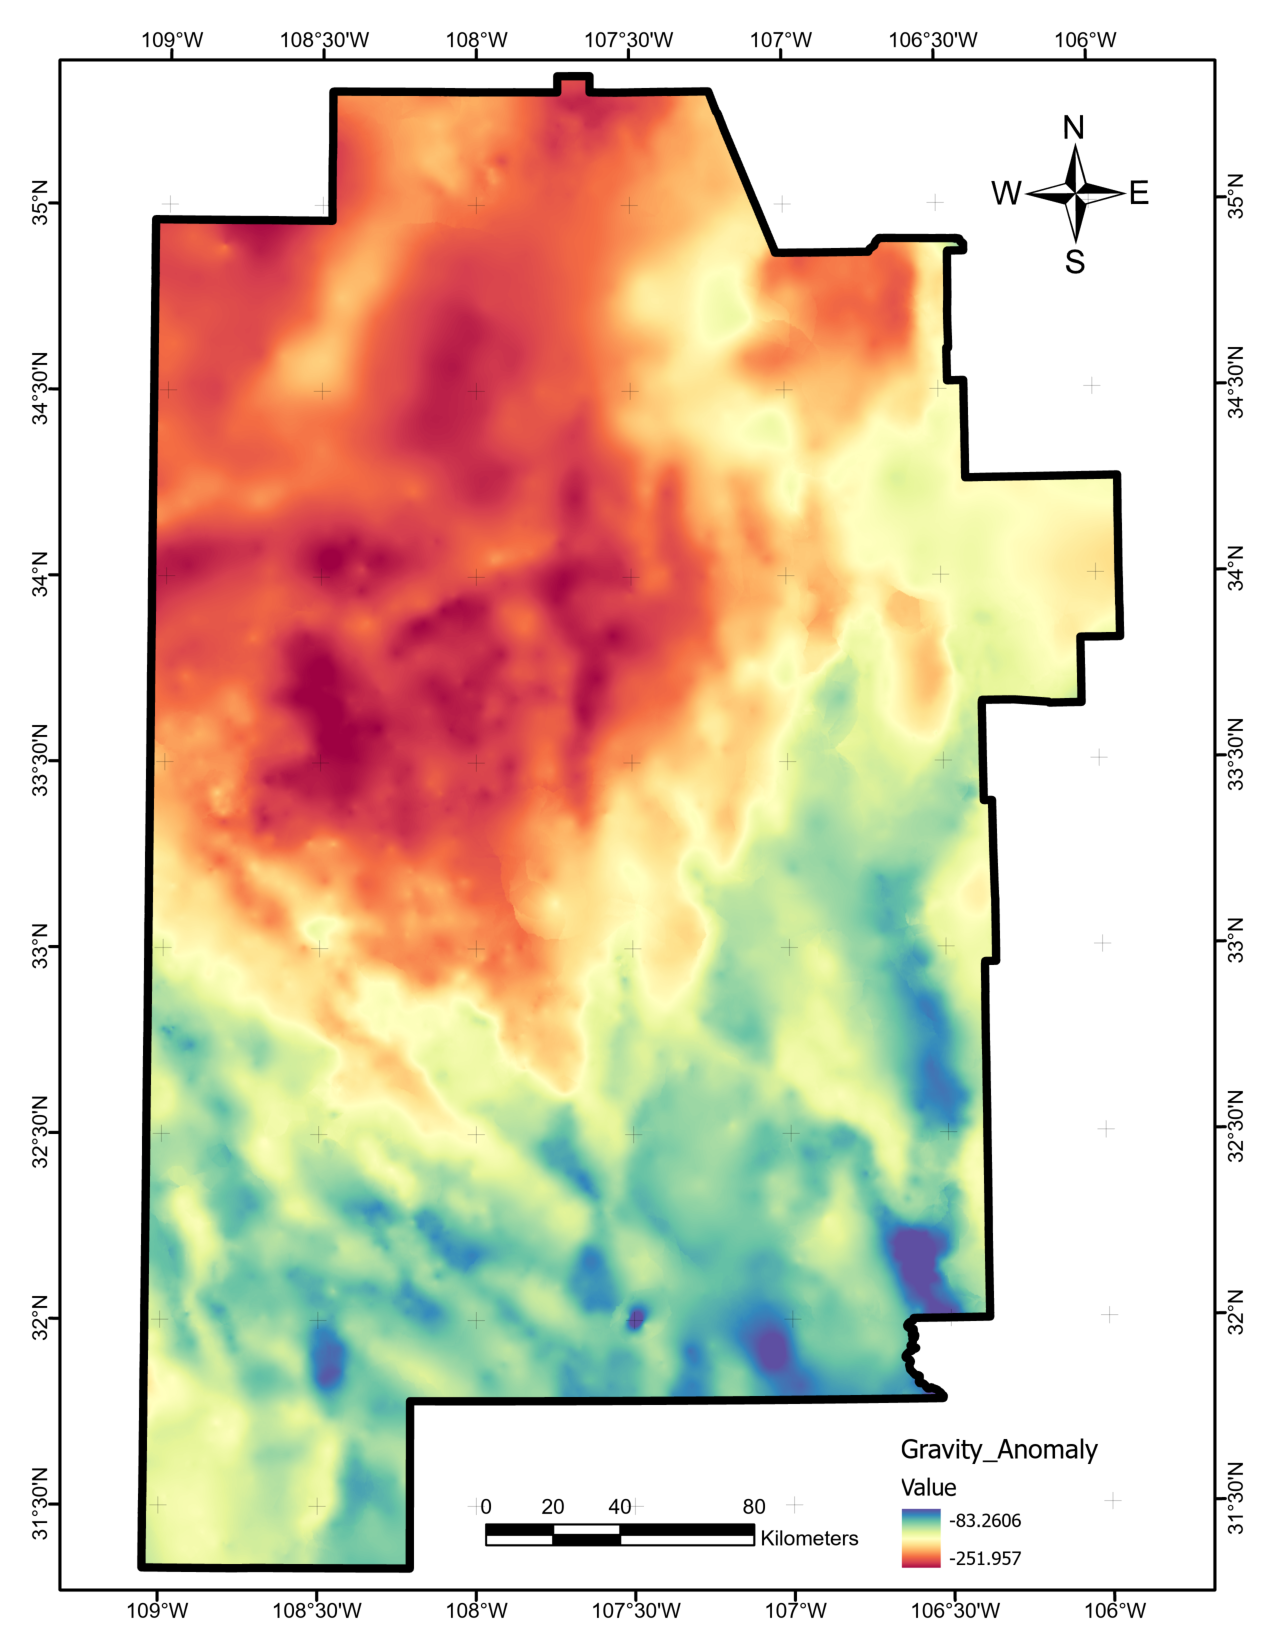
\includegraphics[scale=.50]{templates/images/Figure-GravityAnomaly.pdf}
\caption[Gravity anomaly data layer]{Gravity anomaly data layer. Units are in milligals (mGal). Raster originally created by \protect\citet{bielicki_hydrogeolgic_2015}.}.
\label{fig:feat_gravity}
\end{figure}

\subsubsection{Gravity Anomaly Gradient}

Gradient of the gravity anomaly was calculated using the ArcGIS \textit{Slope} function on the final Gravity Anomaly raster. Parameters used to create the final layer (Figure \ref{fig:feat_gravity_gradient}) include: geodesic method, z unit of meters, and output measurement of degrees.

\begin{figure}[!htp]
\centering
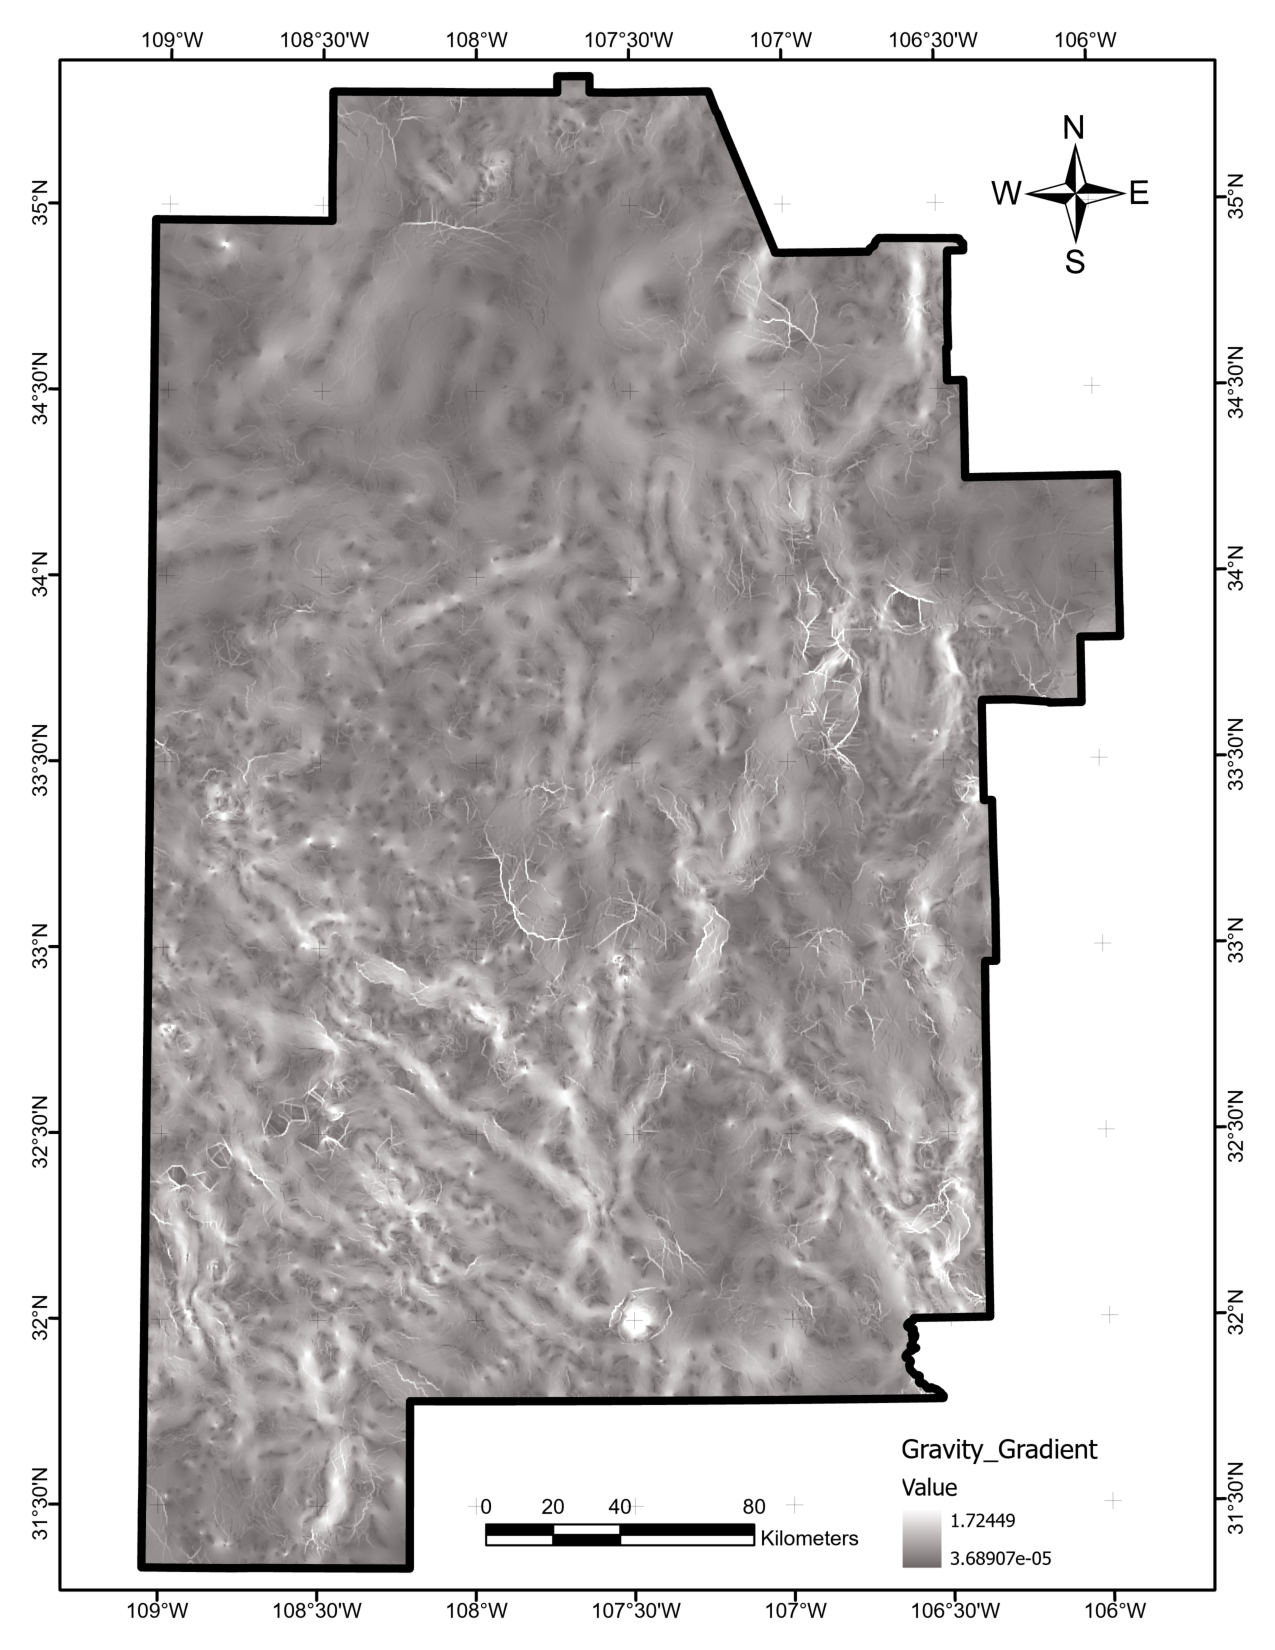
\includegraphics[scale=.50]{templates/images/Figure-GravityGradient.pdf}
\caption[Gravity anomaly gradient data layer]{Gravity anomaly gradient data layer. Units are in mGal/degrees.}.
\label{fig:feat_gravity_gradient}
\end{figure}

\subsubsection{Heat Flow}

The recent $0.5^\circ$ x$0.5^\circ$ resolution heat flow model from \citet{lucazeau_analysis_2019} offers coarse coverage across the southwest NM AOI. The model output was downloaded from the supporting information section of the publication page \citep{lucazeau_analysis_2019}, imported into ArcGIS, and cropped to the Regional Polygon boundaries. After testing several gridding algorithms for a smooth representation of this sparse data, the ArcGIS \textit{Topo to Raster} function produced the best results. The parameters for creating the final layer (Figure \ref{fig:feat_heatflow}) include: tolerance-1 of 2.5, tolerance-2 of 100, drainage enforcement, contour input data, and output cell size of 0.01. 

\begin{figure}[!htp]
\centering
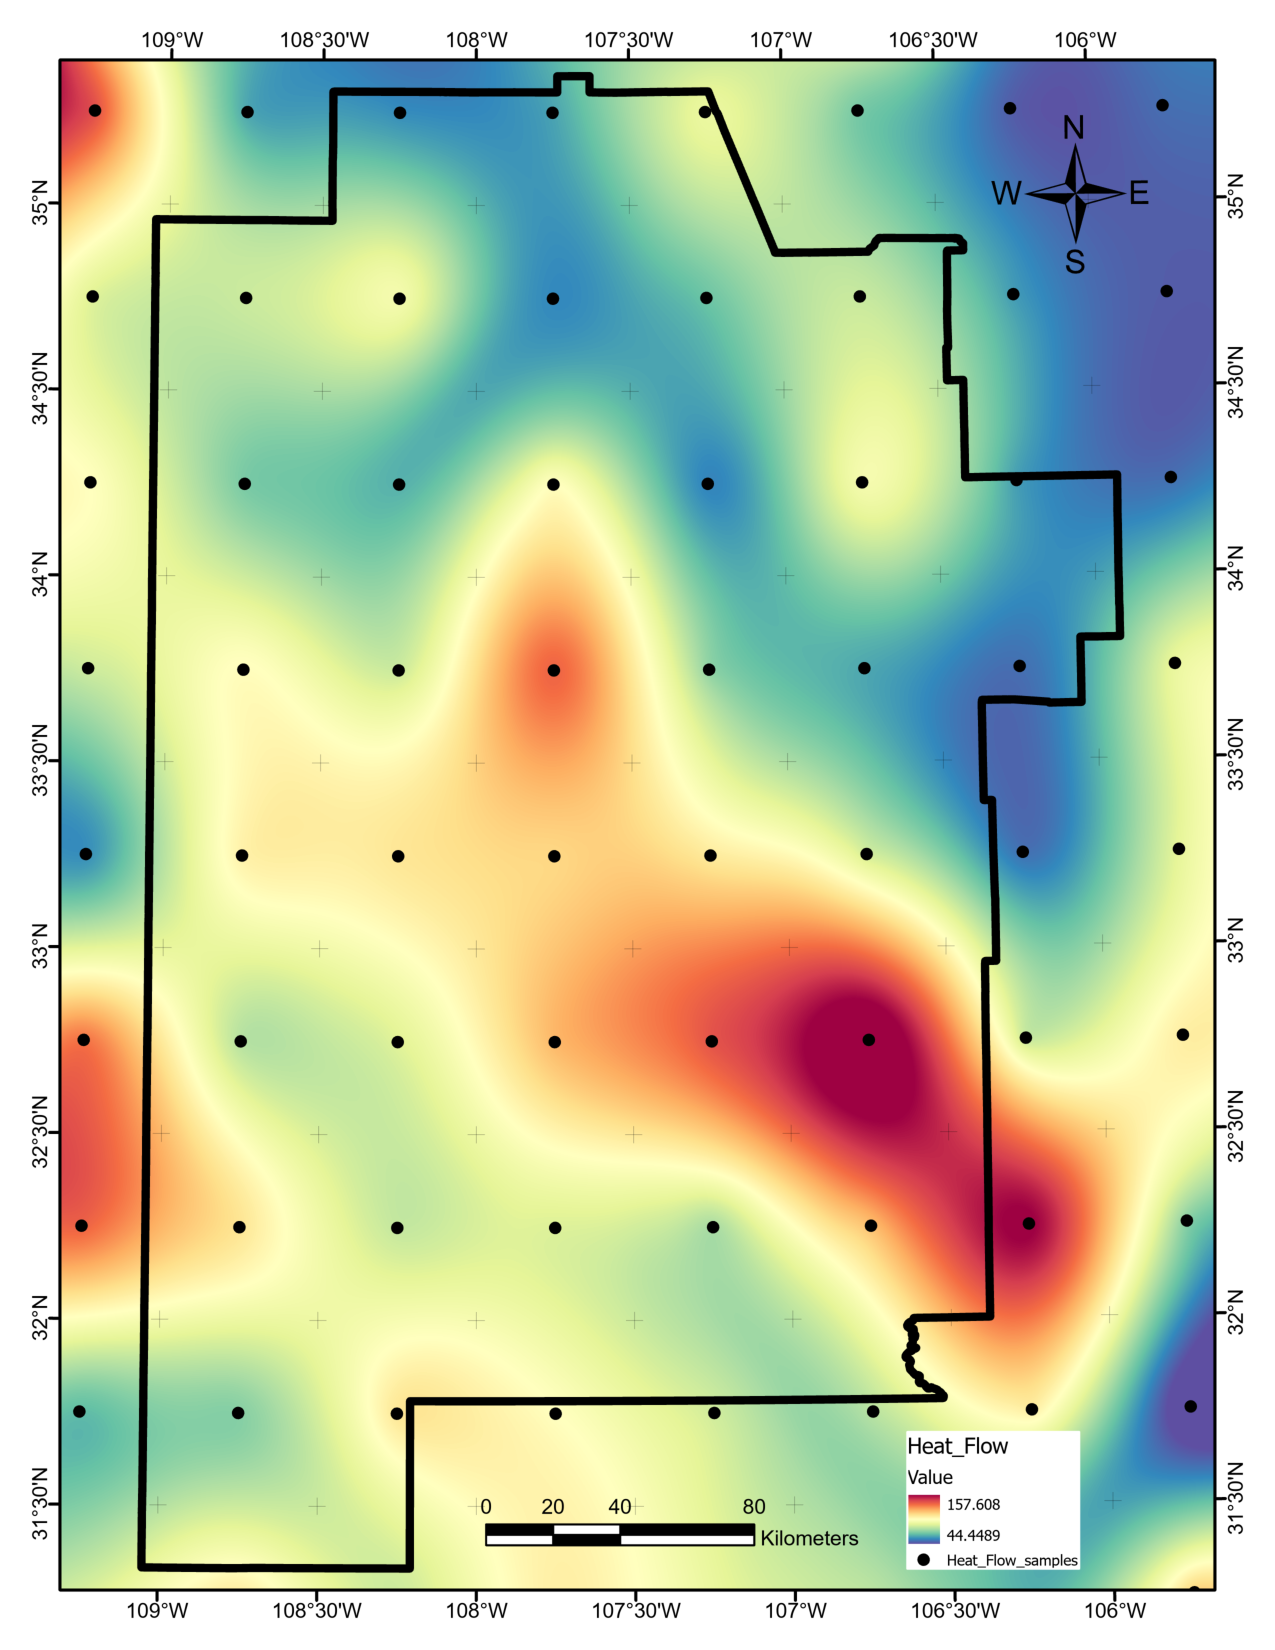
\includegraphics[scale=.50]{templates/images/Figure-HeatFlow.pdf}
\caption[Heat flow data layer]{Heat flow data layer. Units are in W/m-K. Black dots mark the original source data points from \protect\citep{lucazeau_analysis_2019}.}.
\label{fig:feat_heatflow}
\end{figure}

\subsubsection{Lithium Concentration}

Measurements of Lithium concentration were originally assembled by \citet{bielicki_hydrogeolgic_2015} from USGS records, student dissertations, and other sources. These data were downloaded from the OpenEI submission \citep{kelley_geothermal_2015} and merged together using ArcGIS and Python to create a single dataframe of 3,595 measurements, all within the broader Regional Polygon bounds to avoid surface creation edge effects within the tighter AOI. As described for the Boron concentration data layer, attempts to model Lithium concentration using Gaussian Processes provided unsatisfactory results. Instead, the final layer was generated using the ArcGIS \textit{Empirical Bayes Kriging} routine. Selected parameters include: empirical data transformation type, a maximum of 100 points in each local model, 100 simulated semivariograms with k-Bessel model type, and a standard circular search neighborhood with a radius of 1.196 (auto-determined), minimum of 10 neighbors, and maximum of 15 neighbors. The output grid cell size was set to 0.01 degrees. All coincident data were included in the calculation, so any overlapping measurements were considered in generating the final layer (Figure \ref{fig:feat_lithium}).

\begin{figure}[!htp]
\centering
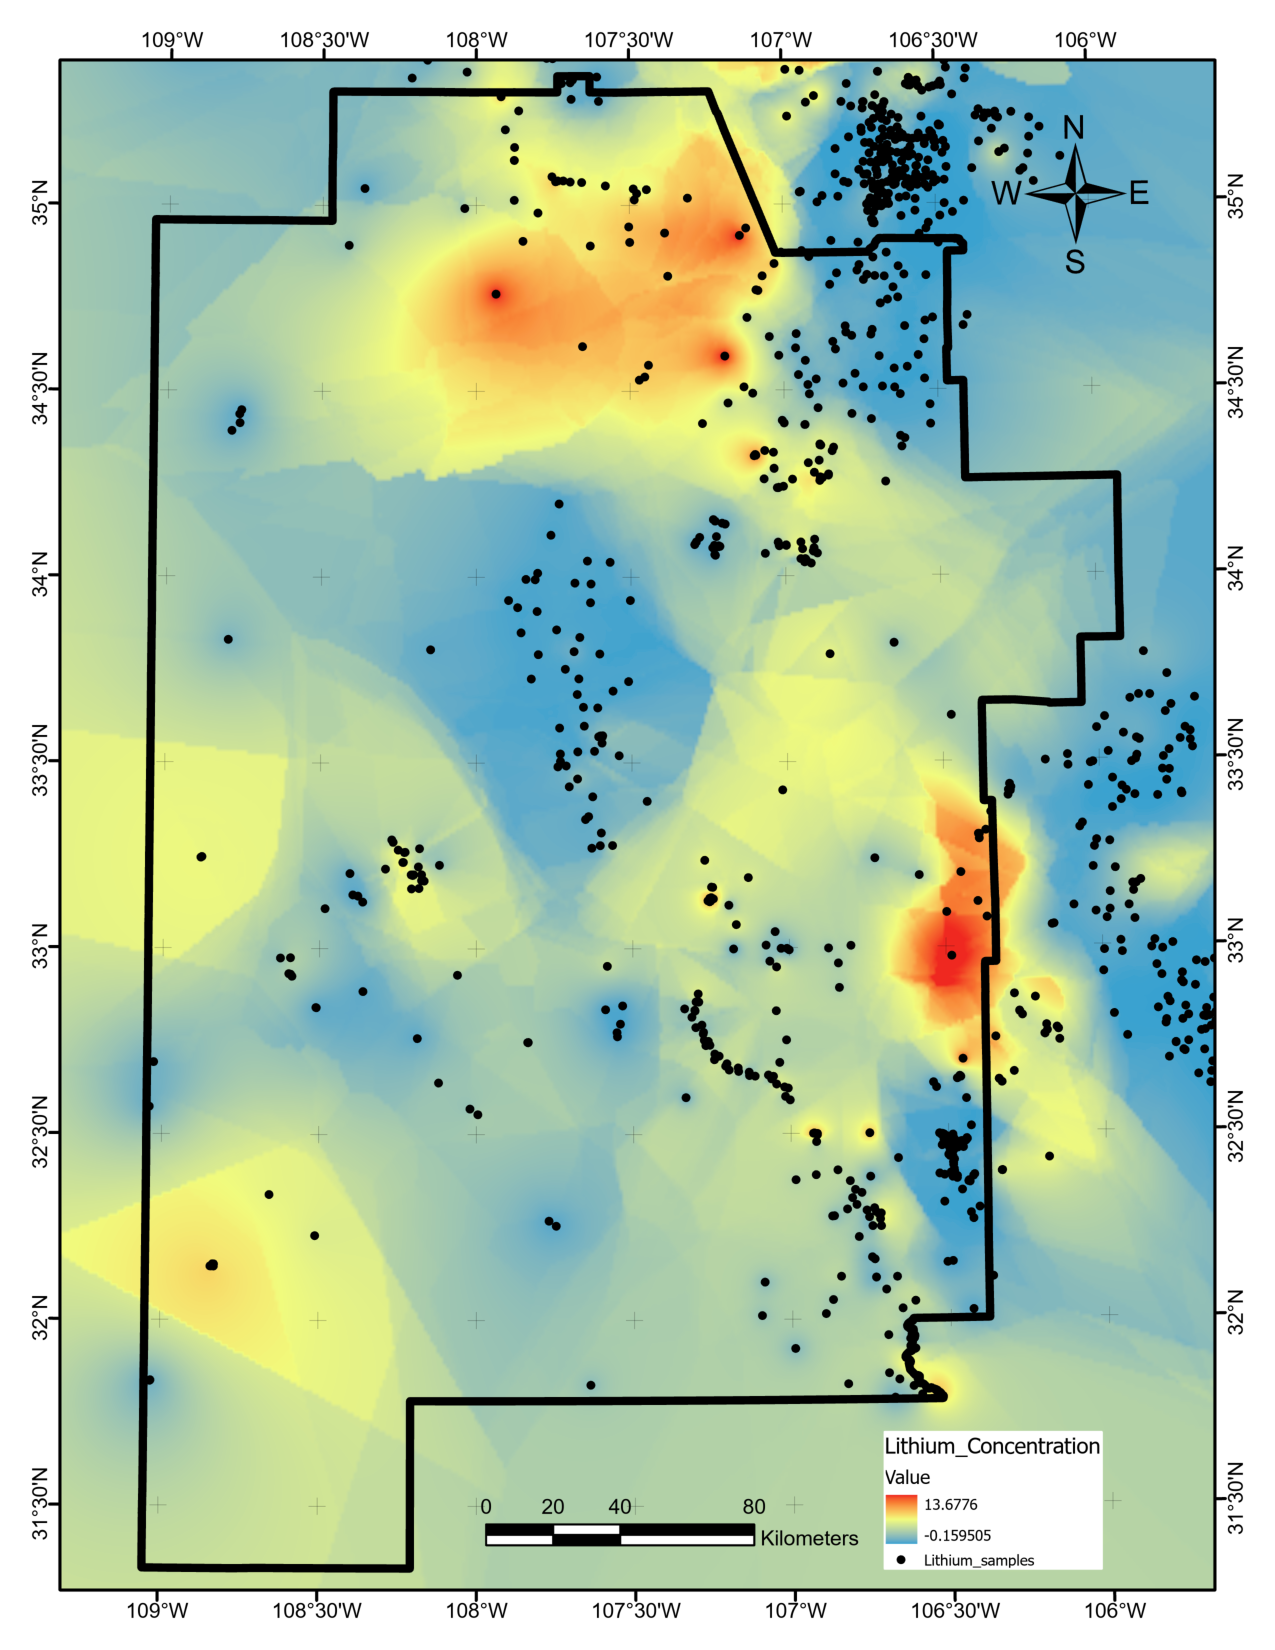
\includegraphics[scale=.50]{templates/images/Figure-Lithium.pdf}
\caption[Lithium concentration data layer]{Lithium concentration data layer. Units are in ppm or mg/L. Black dots mark sample locations in the complete data set from \protect\citep{bielicki_hydrogeolgic_2015}}.
\label{fig:feat_lithium}
\end{figure}

\subsubsection{Magnetic Anomaly}

USGS magnetic anomaly data derived from aerial surveys \citep{bankey_digital_2002} were used in both the southwest NM PFA analysis \citep{bielicki_hydrogeolgic_2015} and cluster analysis \citep{pepin_new_2018}. After downloading the raster from the PFA OpenEI submission \citep{kelley_geothermal_2015}, it was imported directly into ArcGIS. The layer (Figure \ref{fig:feat_magnetics}) required no further processing.

\begin{figure}[!htp]
\centering
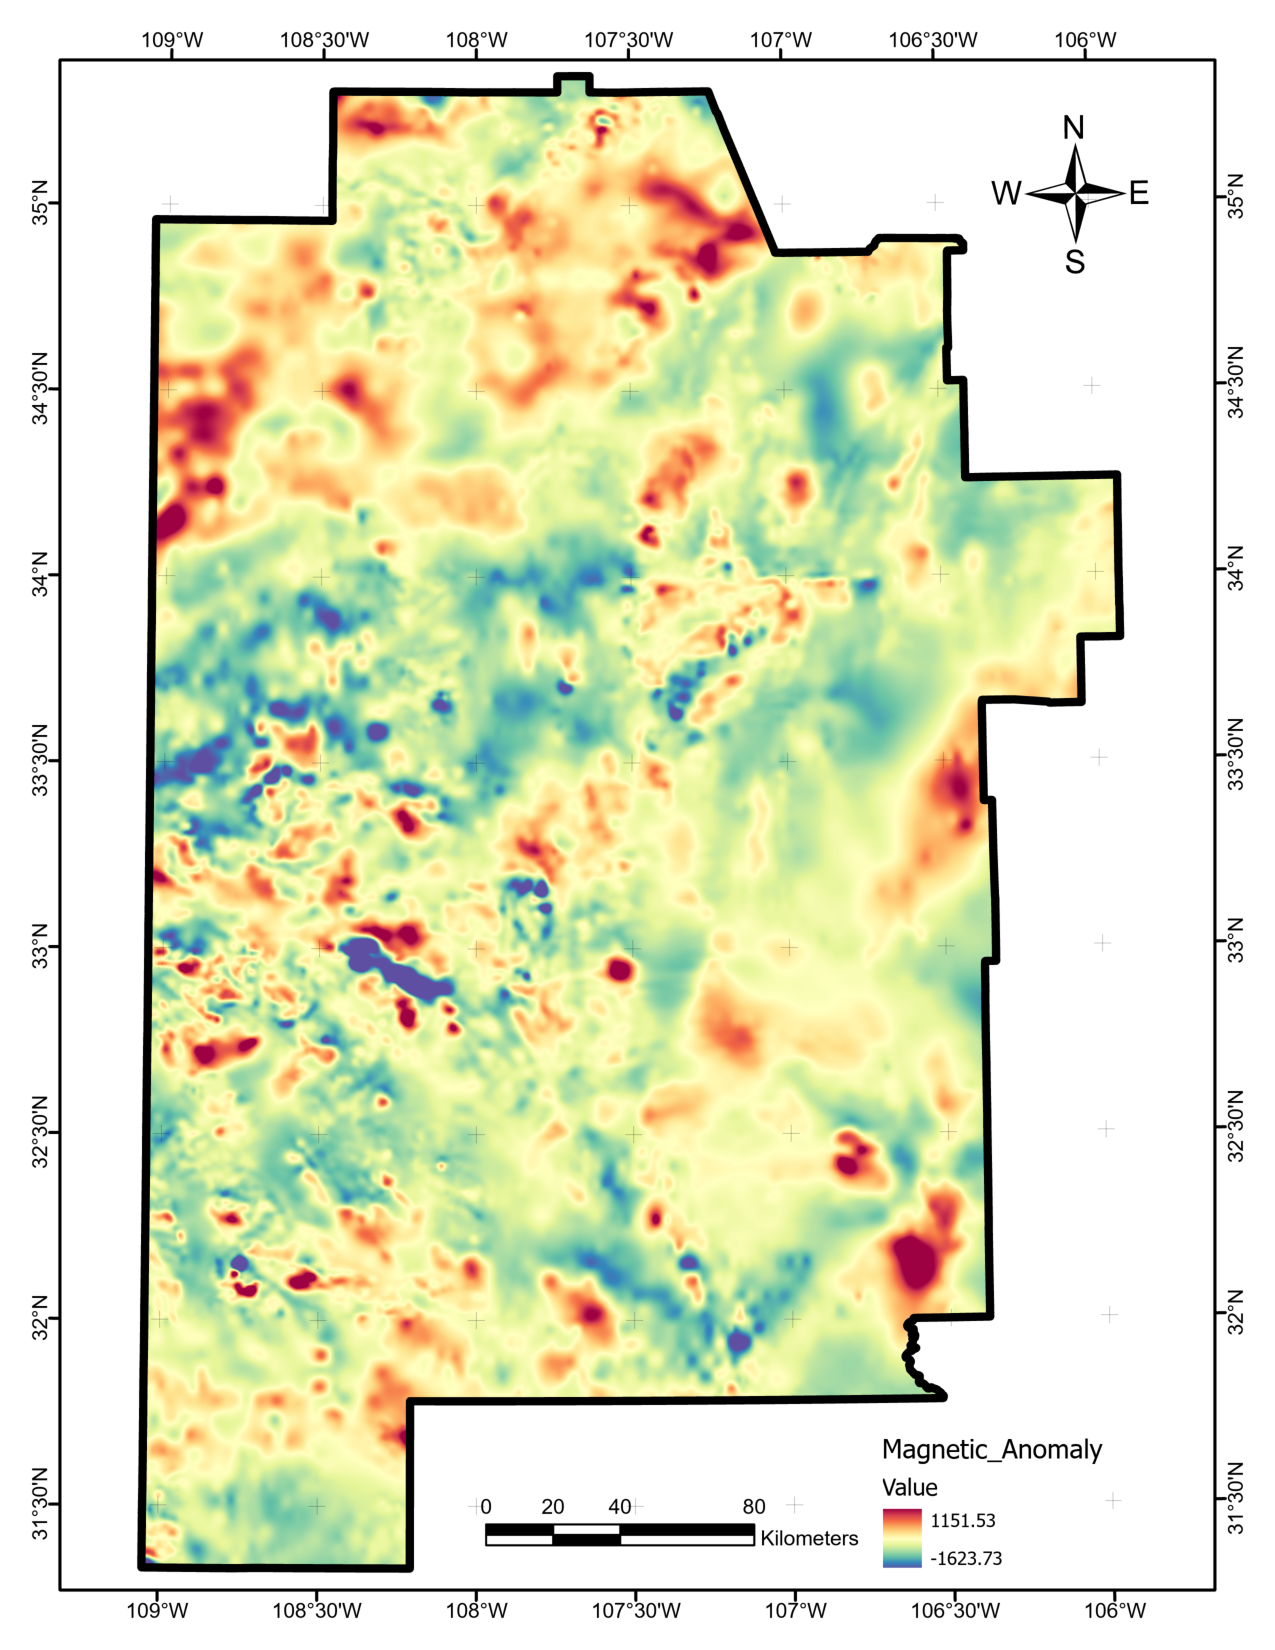
\includegraphics[scale=.50]{templates/images/Figure-MagneticAnomaly.pdf}
\caption[Magnetic anomaly data layer]{Magnetic anomaly data layer. Units are in nanoteslas (nT). Raster originally created by \protect\citet{bielicki_hydrogeolgic_2015}.}.
\label{fig:feat_magnetics}
\end{figure}

\subsubsection{Magnetic Anomaly Gradient}

The gradient of the magnetic anomaly was calculated using the ArcGIS \textit{Slope} function on the final Magnetic Anomaly raster. Parameters selected to create this layer (Figure \ref{fig:feat_magnetic_gradient}) include: geodesic method, z unit of meters, and output measurement of degrees.

\begin{figure}[!htp]
\centering
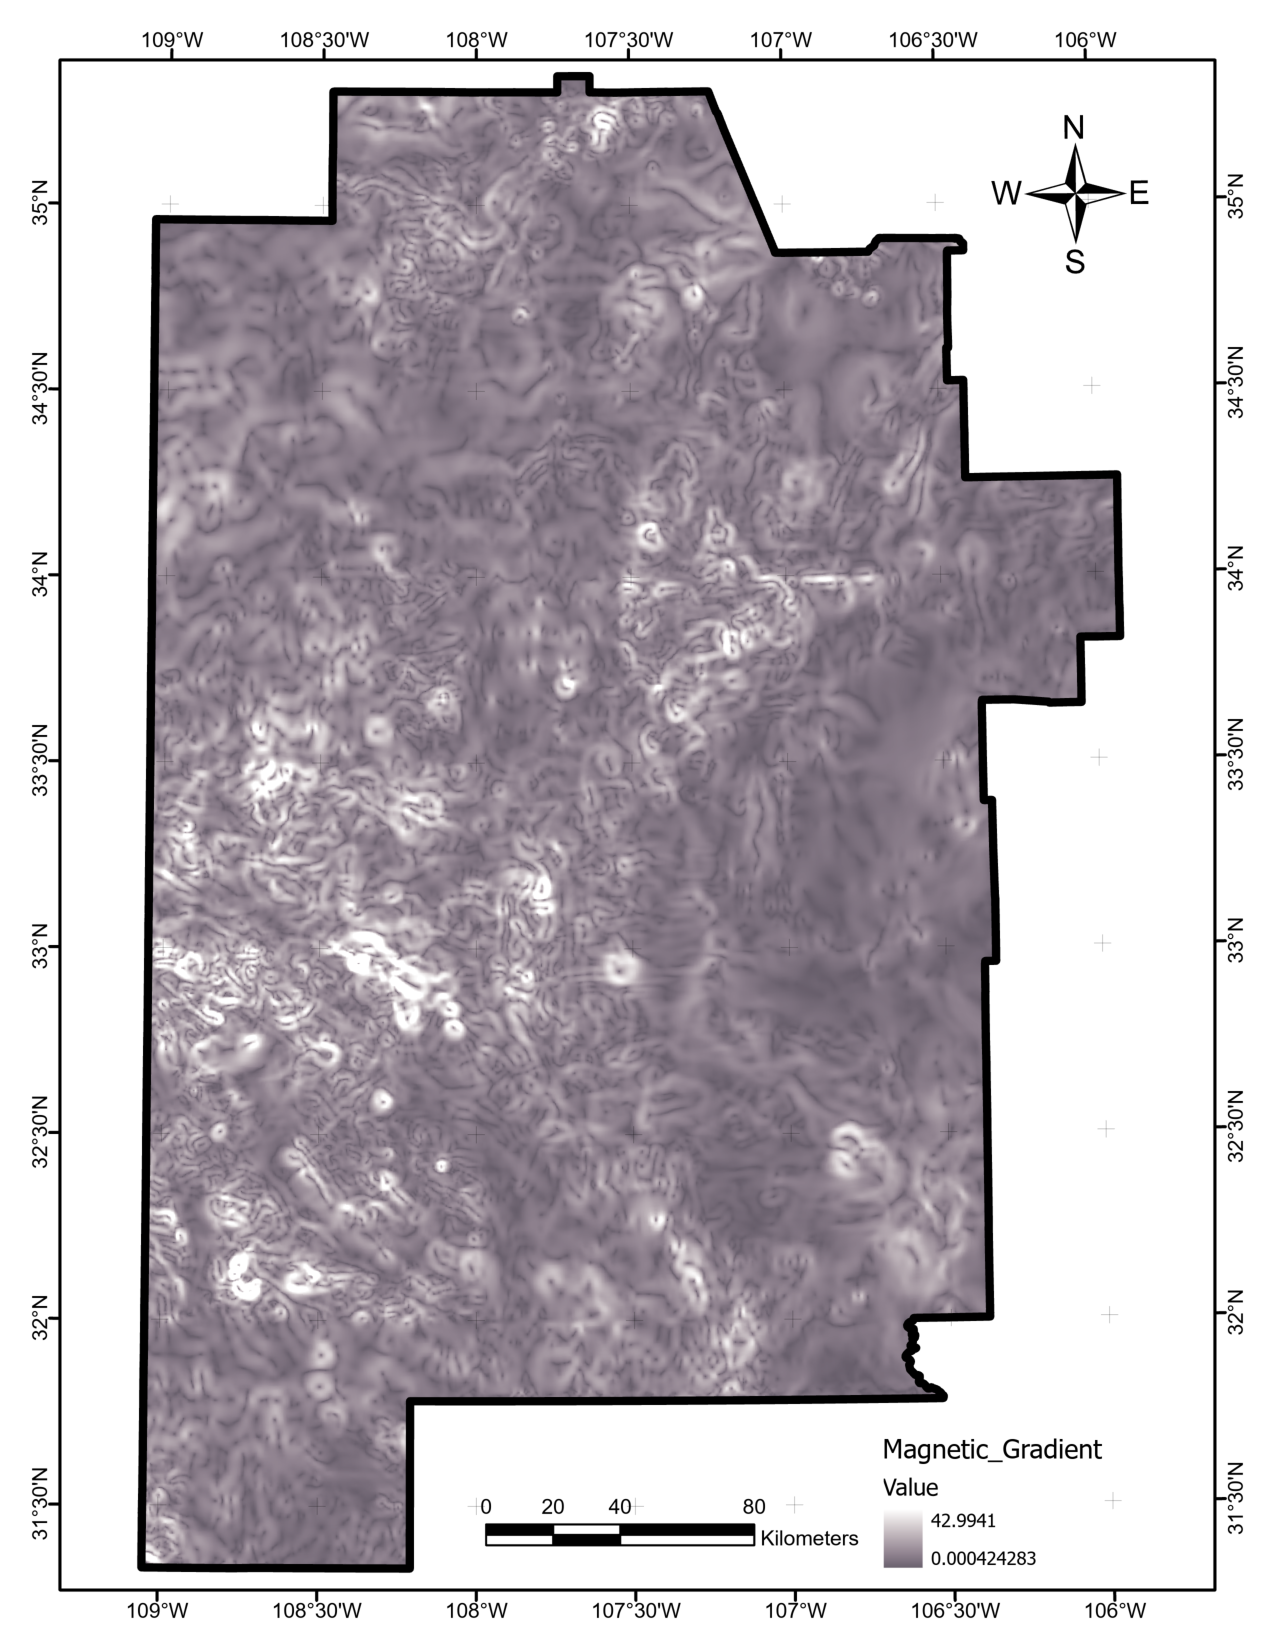
\includegraphics[scale=.50]{templates/images/Figure-MagneticGradient.pdf}
\caption[Magnetic anomaly gradient data layer]{Magnetic anomaly gradient data layer. Units are in nT/degrees.}.
\label{fig:feat_magnetic_gradient}
\end{figure}

\subsubsection{Quaternary Fault Density}

Faults showing Quaternary displacement were digitized at the 1:24,000 scale by the New Mexico Bureau of Geology and Mineral Resources and provided to \citet{bielicki_hydrogeolgic_2015} and \citet{pepin_new_2018} in support of their investigations. The associated polyline features were downloaded from the PFA OpenEI submission \citep{kelley_geothermal_2015} and loaded into ArcGIS. As discussed for the Drainage Density layer, a Python-based kernel density workflow using extracted points from these polylines failed to produce satisfactory results. Instead, the ArcGIS \textit{Kernel Density} function was applied to create the final layer map (Figure \ref{fig:feat_qfaults}). Selected parameters for this function include an output cell size of 0.0025 degrees and auto-determined search radius of 0.367.

\begin{figure}[!htp]
\centering
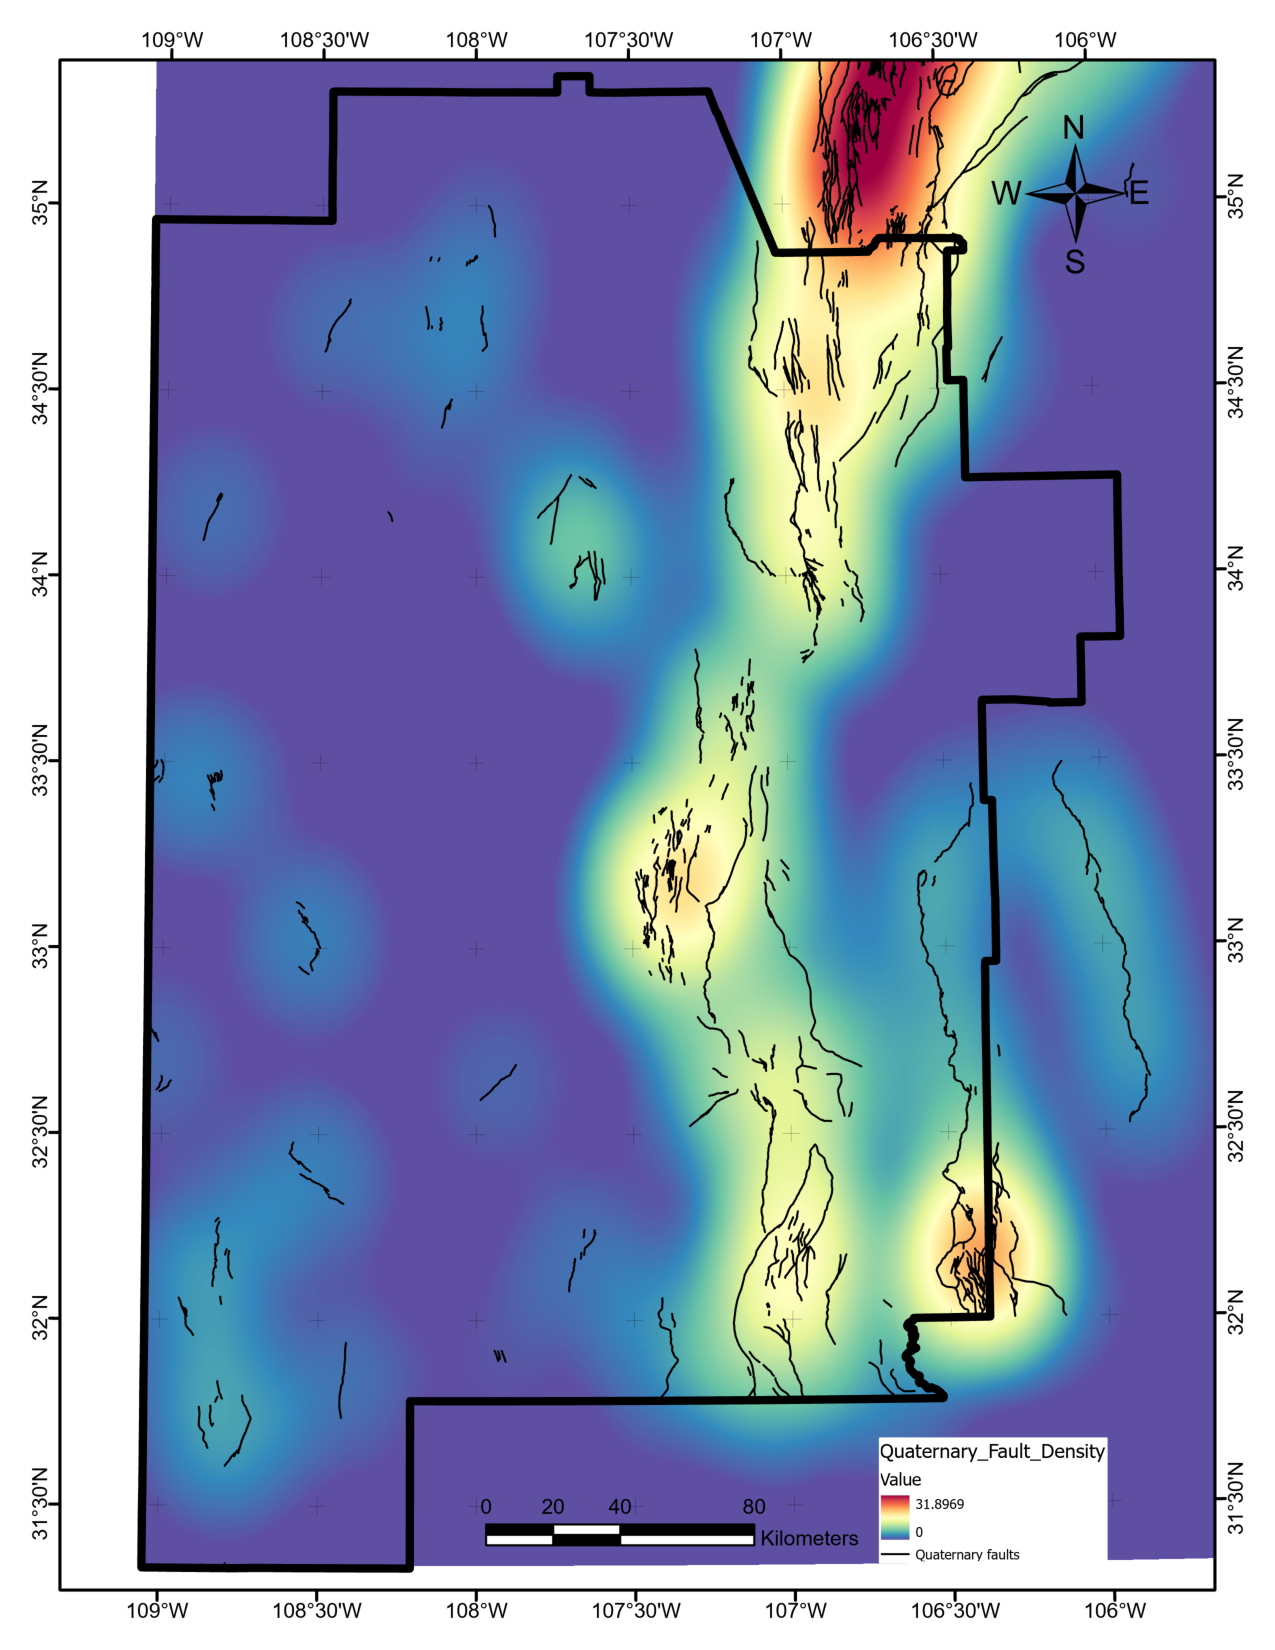
\includegraphics[scale=.50]{templates/images/Figure-QFaultDensity.pdf}
\caption[Quaternary fault density data layer]{Quaternary fault density data layer. Units are in degrees/degrees$^2$. Black lines show the fault polyline data set archived by \protect\citet{bielicki_hydrogeolgic_2015}.}.
\label{fig:feat_qfaults}
\end{figure}

\subsubsection{Silica Geothermometer Temperature}

Silica concentration data from across the study area were compiled by \citet{bielicki_hydrogeolgic_2015}, and converted to reservoir temperatures using the Fournier chalcedony geothermometer relationship \citep{fournier_chemical_1977}. These data were downloaded from the southwest NM PFA OpenEI submission \citep{kelley_geothermal_2015} and merged together using ArcGIS and Python to create a single dataframe of 7,259 measurements, all within the broader Regional Polygon bounds to avoid surface creation edge effects within the tighter AOI. As described for the Boron Concentration data layer, attempts to model Si geothermometer estimates using Gaussian Processes provided unsatisfactory results. Instead, the final layer was created using the ArcGIS \textit{Empirical Bayes Kriging} routine. Selected parameters include: empirical data transformation type, a maximum of 100 points in each local model, 100 simulated semivariograms with k-Bessel model type, and a standard circular search neighborhood with a radius of 1.196 (auto-determined), minimum of 10 neighbors, and maximum of 15 neighbors. The output grid cell size was set to 0.01 degrees. All coincident data were included in the calculation, so any overlapping measurements were considered in generating the final layer (Figure \ref{fig:feat_si_temp}).

\begin{figure}[!htp]
\centering
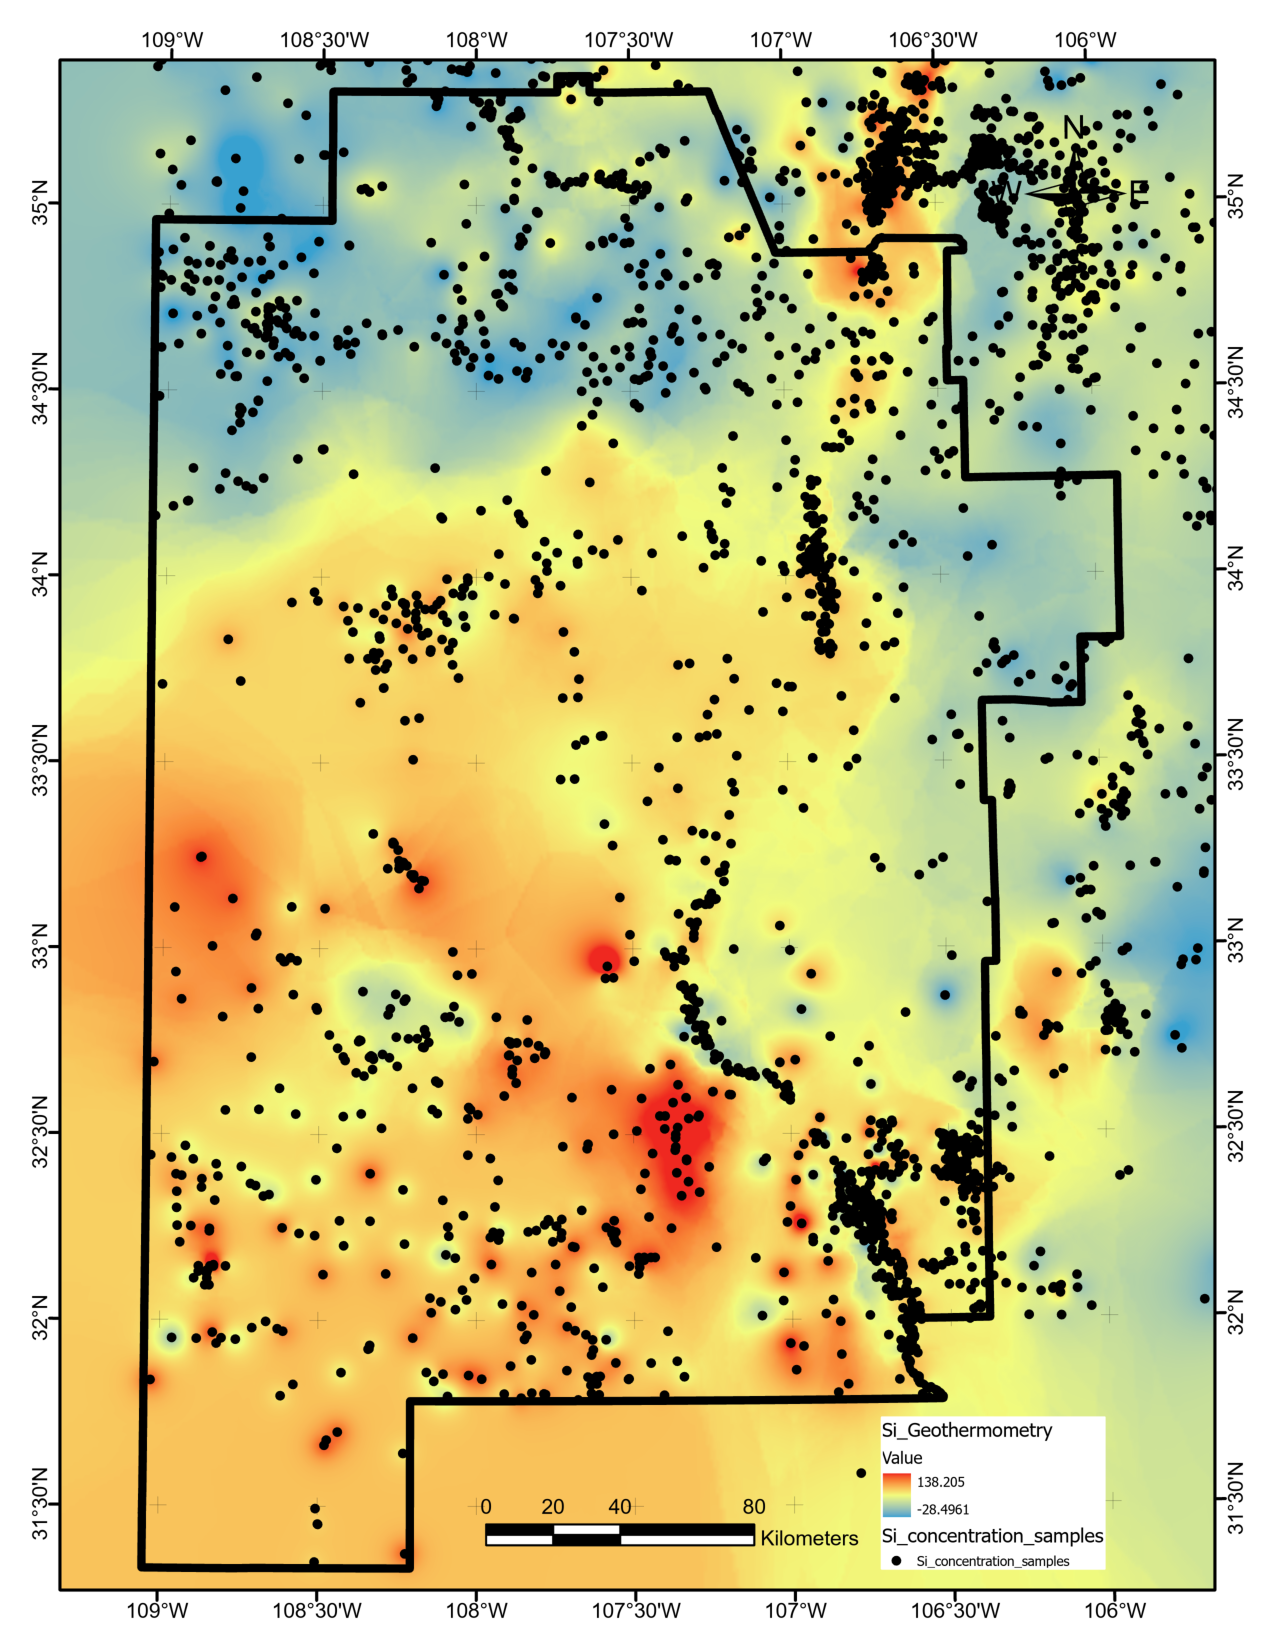
\includegraphics[scale=.50]{templates/images/Figure-SiTemp.pdf}
\caption[Silica geothermometer temperature data layer]{Chalcedony geothermometer data layer. Units are in $^\circ$C. Black dots indicate locations where silica concentration was sampled, as collected by \protect\citet{bielicki_hydrogeolgic_2015}}.
\label{fig:feat_si_temp}
\end{figure}

\subsubsection{Spring Density}
%%\captionsetup[figure]{skip=0pt}
\begin{wrapfigure}{R}{0.5\linewidth}
\centering
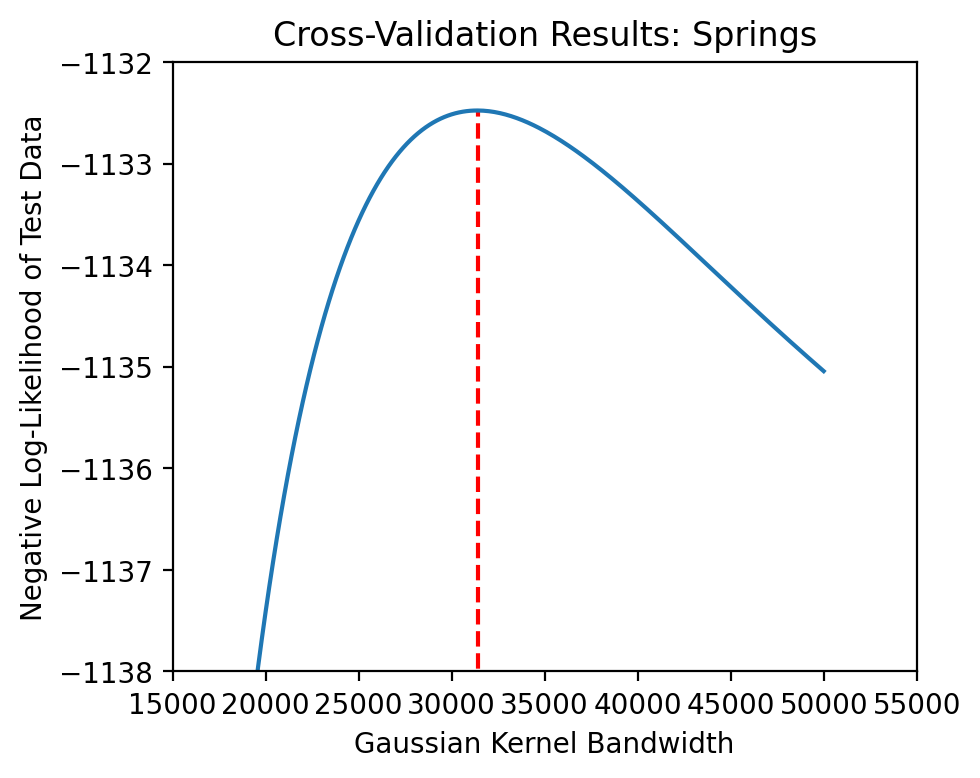
\includegraphics[scale=0.6]{templates/images/Figure-Springs_kde_gridsearchcv_result.png}
\singlespacing
\caption[Spring density parameter tuning]{Cross-validation results for springs KDE. Red dashed line indicates maximum negative log likelihood value identifying the best kernel radius.}
\label{fig:spring_cv}
%%\captionsetup[figure]{skip=10pt}
\end{wrapfigure}
The locations of springs across the study area were downloaded from the USGS National Water Information System \citep{usgs_national_2021}. A total of 2,565 springs were recorded within the geographic bounds of the Regional Polygon. As with the Earthquake Density layer, this point set was loaded into a KDE Python script, which used a grid search routine to determine the best kernel radius for a Gaussian kernel density operator. Ten-fold cross validation identified the best radius value of 31,400 m (Figure \ref{fig:spring_cv}). 

KDE values calculated at each fishnet point location were loaded into ArcGIS, and \textit{Kriging} was used to generate a final layer for plotting purposes (Figure \ref{fig:feat_spring}). Selected \textit{Kriging} parameters included a spherical semivariogram model, lag size of 1e-6, variable search radius with 12-point requirement, and output cell size of 0.01. 

\begin{figure}[!htp]
\centering
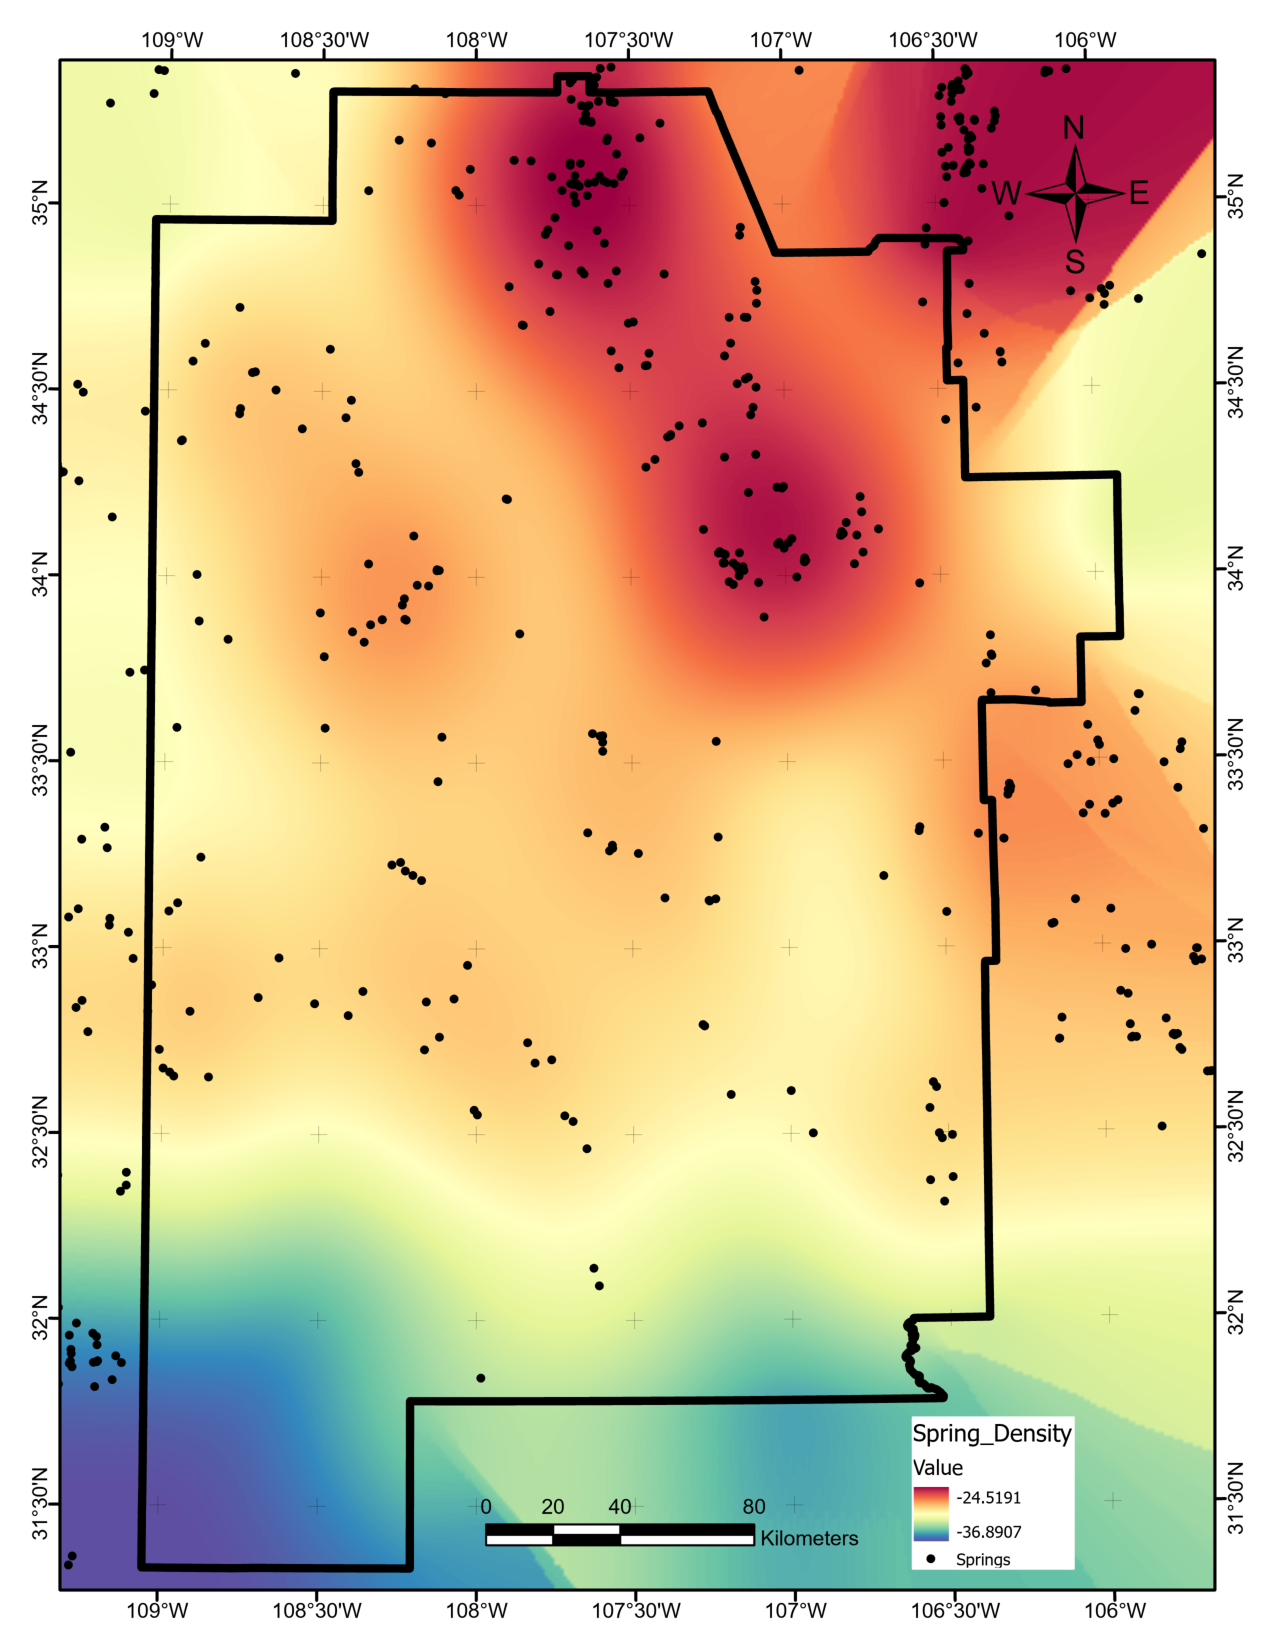
\includegraphics[scale=.50]{templates/images/Figure-SpringDensity.pdf}
\caption[Spring density data layer]{Spring density data layer. Units are in log(points/km$^2$). Black dots indicate spring locations from \protect\citep{usgs_national_2021}.}
\label{fig:feat_spring}
\end{figure}

\subsubsection{State Map Fault Density}

Digitized state geologic map fault outlines are available for download from the USGS Energy and Environment in the Rocky Mountain Area data portal \citep{usgs_eerma_2021}, including New Mexico faults \citep{stoeser_new_2005}. This data layer was loaded into ArcGIS and, like the Quaternary fault data set, converted to a density layer using the \textit{Kernel Density} operation (Figure \ref{fig:state_faults}). Selected parameters for this function include an output cell size of 0.0025 degrees and an auto-determined search radius of 0.252.

\begin{figure}[!htp]
\centering
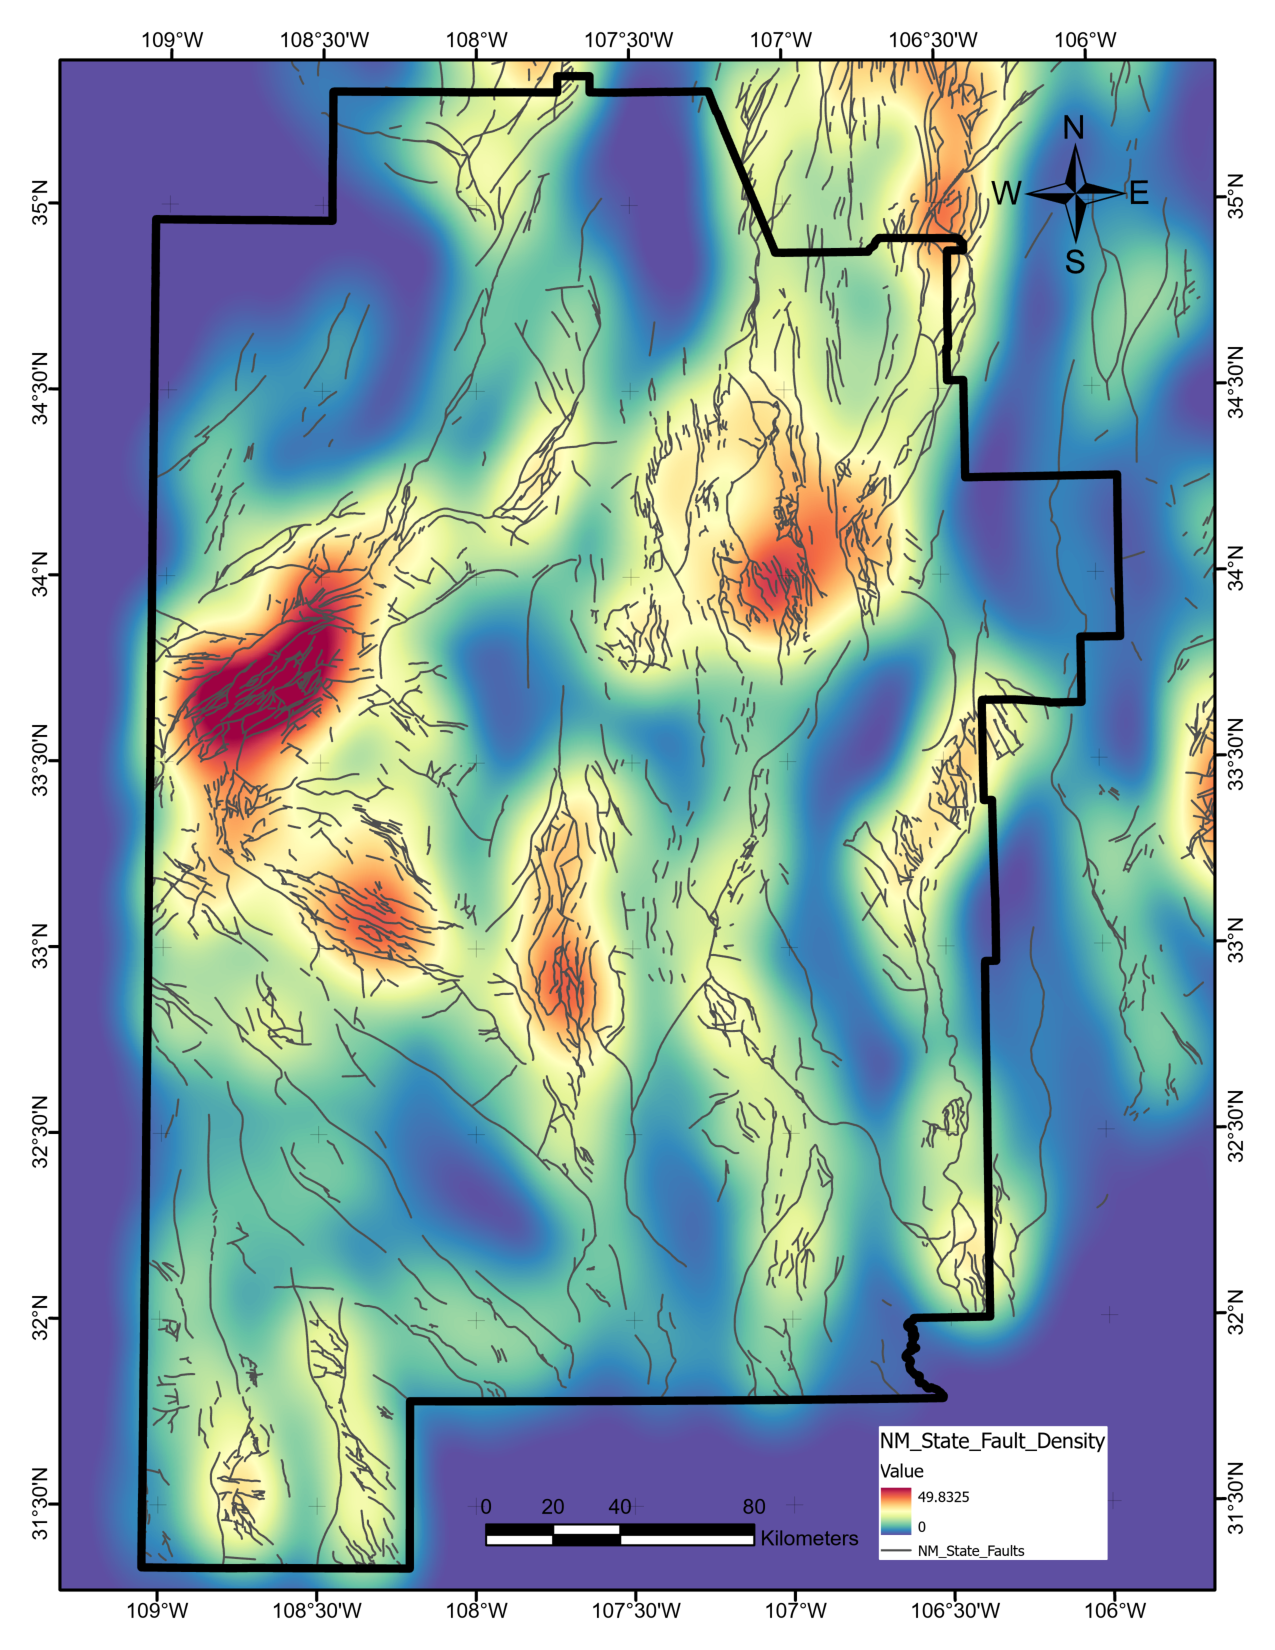
\includegraphics[scale=.50]{templates/images/Figure-StateFaultDensity.pdf}
\caption[State fault density data layer]{State fault density data layer. Units are in degrees/degrees$^2$. Dark gray lines trace the fault polyline data set obtained from USGS Open-File Report 2005-1351 \protect\citep{stoeser_new_2005}}
\label{fig:state_faults}
\end{figure}

\subsubsection{Surface Topography (DEM)}

The southwest NM PFA data archive \citep{kelley_geothermal_2015} includes a \acrlong{dem} (\acrshort{dem}) layer with surface elevations at a 1 arc-sec resolution. This layer was downloaded and imported into ArcGIS, however a data gap along the easternmost section of the AOI required the addition of two $1^\circ$x$1^\circ$ DEM tiles at the same resolution to fully complete the layer. These tiles were downloaded from the USGS The National Map website \citep{usgs_tnm_2021} and merged with the original DEM. The final layer (Figure \ref{fig:feat_dem}) required no further processing.

\begin{figure}[!htp]
\centering
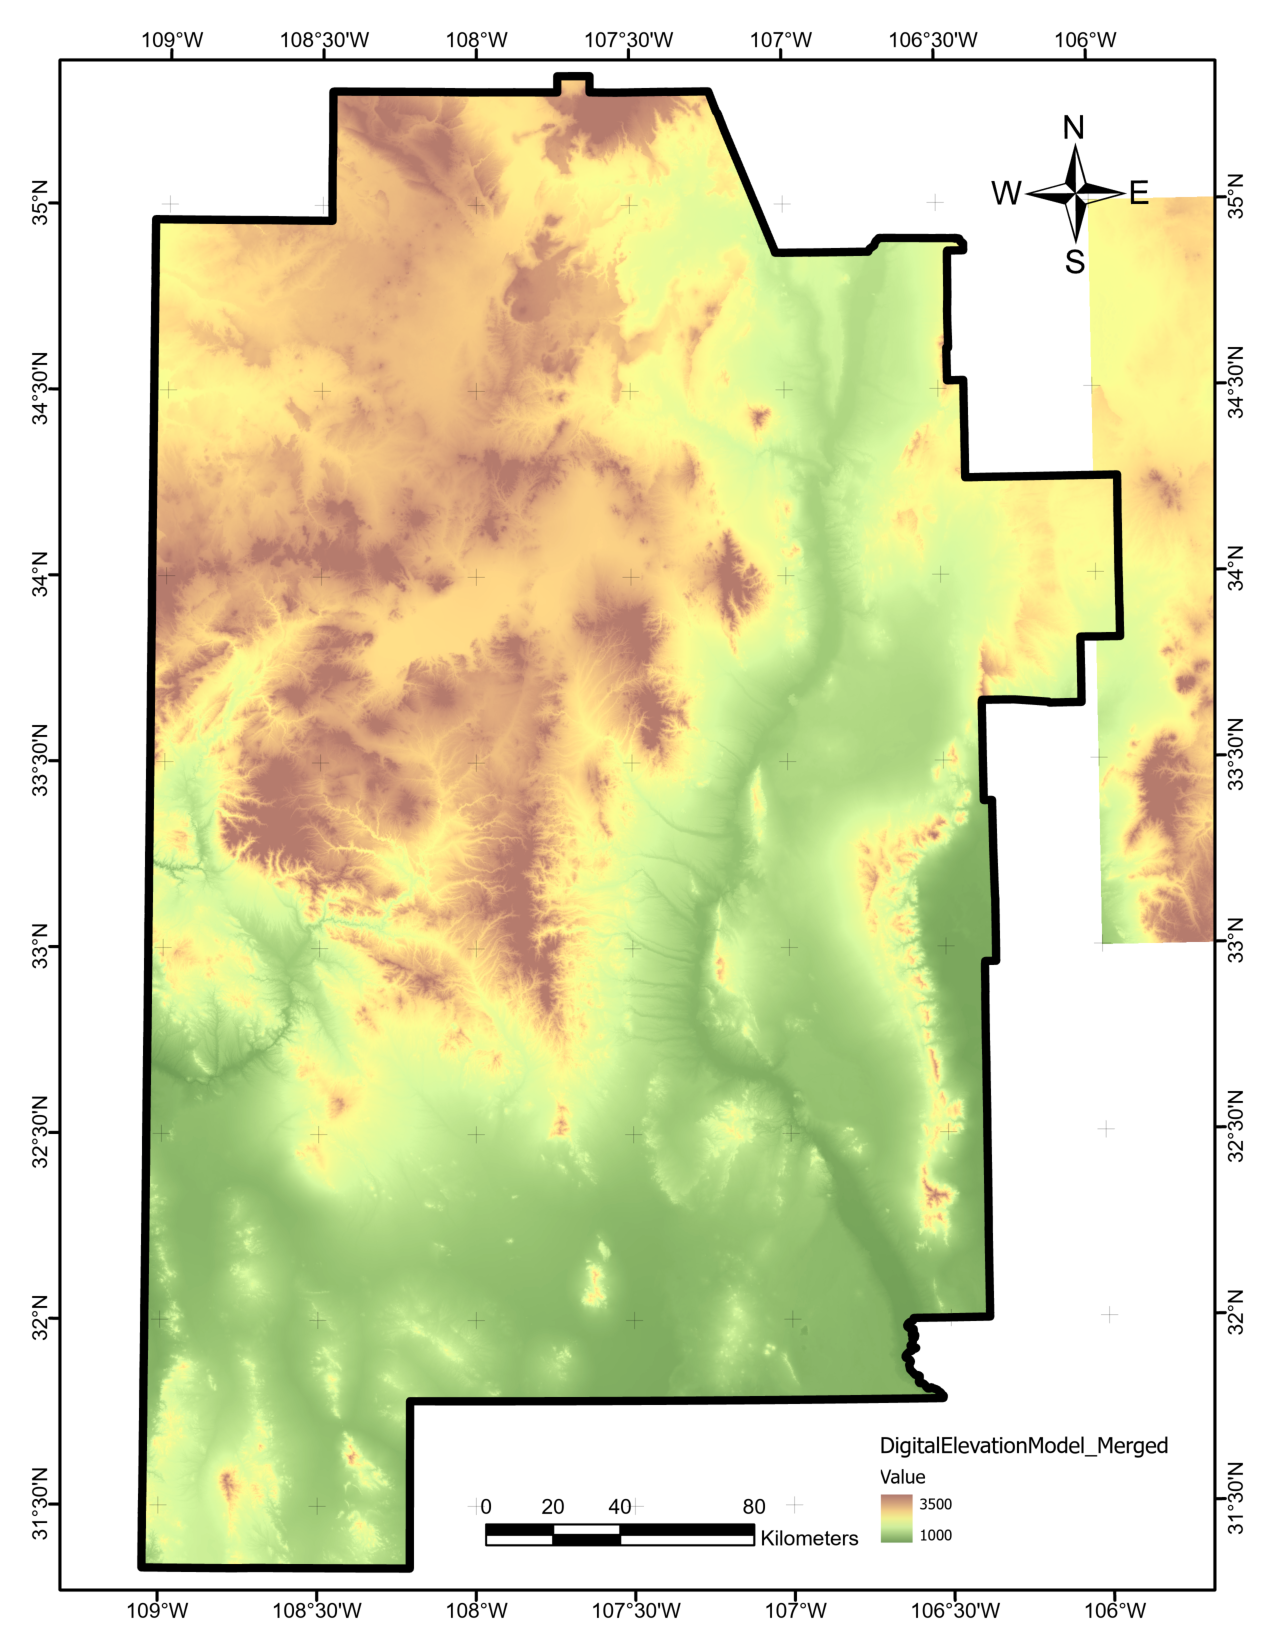
\includegraphics[scale=.50]{templates/images/Figure-DEM.pdf}
\caption[Surface topography (DEM) data layer]{Surface topography (DEM) data layer. Units are in meters. Layer combines the DEM raster from \citep{bielicki_hydrogeolgic_2015} with data from The National Map online \citep{usgs_tnm_2021}.}
\label{fig:feat_dem}
\end{figure}

\subsubsection{Topographic Gradient}

Surface elevation gradient was calculated using the ArcGIS \textit{Slope} function on the final DEM layer. Parameters selected to create this layer (Figure \ref{fig:feat_dem_gradient}) include: geodesic method, z unit of meters, and output measurement of degrees.

\begin{figure}[!htp]
\centering
\includegraphics[scale=.50]{templates/images/Figure-DEMGradient.pdf}
\caption[Topographic gradient data layer]{Topographic gradient data layer. Units are in meters/degrees.}
\label{fig:feat_dem_gradient}
\end{figure}

\subsubsection{Volcanic Dike Density}

The USGS Energy and Environment in the Rocky Mountain Area data portal \citep{usgs_eerma_2021} also includes digitized volcanic dike outlines from the New Mexico state geologic map \citep{stoeser_new_2005-1}. This data set was imported into ArcGIS and, like the Quaternary fault data set, converted to a density layer using the \textit{Kernel Density} operation (Figure \ref{fig:feat_dikes}). Selected parameters for this function included an output cell size of 0.0025 degrees and an auto-determined search radius of 0.252.

\begin{figure}[!htp]
\centering
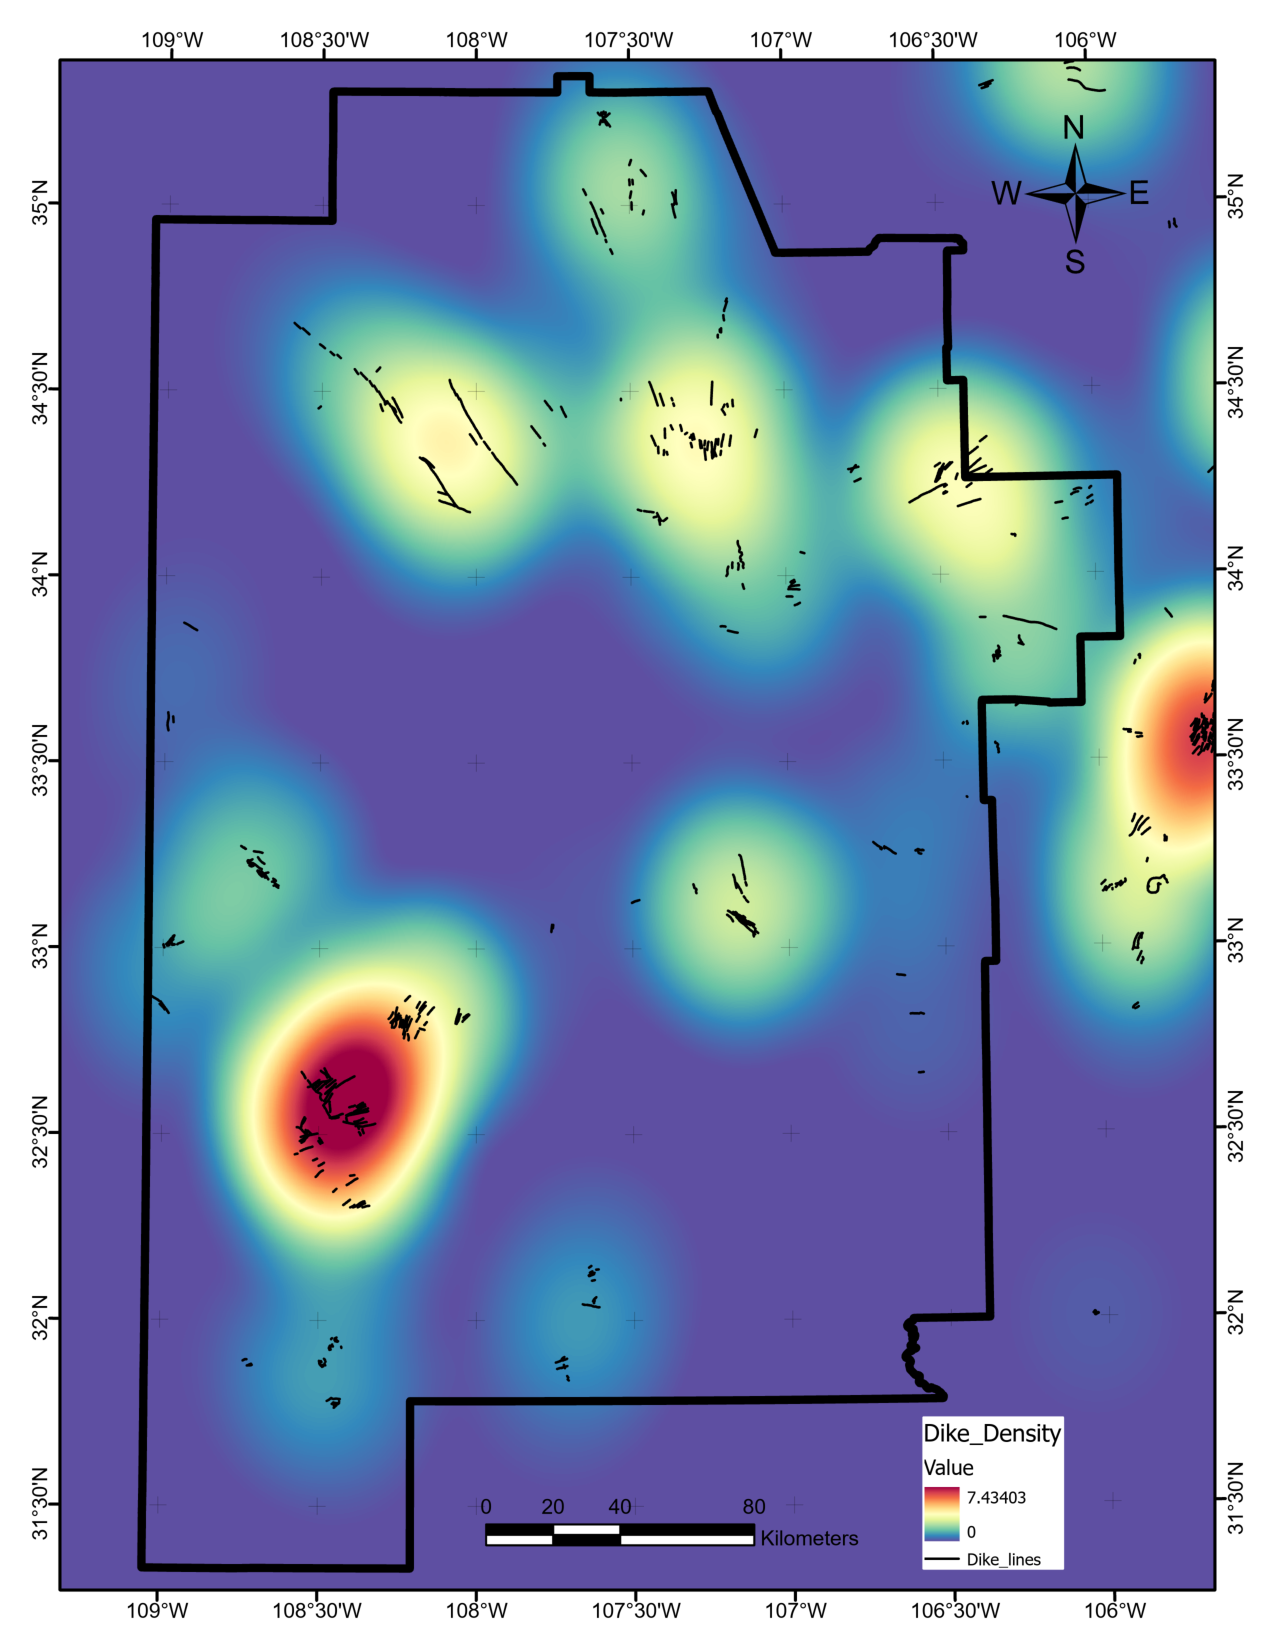
\includegraphics[scale=.50]{templates/images/Figure-DikeDensity.pdf}
\caption[Volcanic dike data layer]{Volcanic dike density data layer. Units are in degrees/degrees$^2$. Black lines trace the dike polyline data set obtained from USGS Open-File Report 2005-1351 \protect\citep{stoeser_new_2005-1}.}
\label{fig:feat_dikes}
\end{figure}

\subsubsection{Volcanic Vent Density}

Volcanic vents identified in the study area were retrieved from the New Mexico Bureau of Geology and Mineral Resources using the NMBGMR Interactive Map \citep{nmbgmr_nmbgmr_2021}. A total of 811 volcanic vents are observed within the geographic bounds of the Regional Polygon. As with the Earthquake Density layer, the point set was loaded into a KDE Python script, which used a grid search routine to determine the optimal kernel radius. Ten-fold cross validation suggested a radius of 28,300 m (Figure \ref{fig:vent_cv}).

\begin{figure}[!htp]
\centering
%%\singlespacing
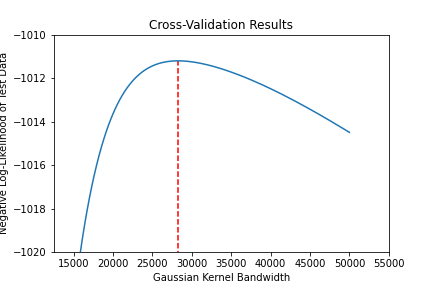
\includegraphics[scale=.60]{templates/images/Figure-Vents_kde_gridsearchcv_result.png}
\caption[Volcanic vent density parameter tuning]{Cross-validation results for volcanic vent KDE. Red dashed line indicates maximum negative log likelihood value identifying the best kernel radius.}
\label{fig:vent_cv}
\end{figure}

KDE values calculated at each fishnet point location were loaded into ArcGIS, and \textit{Kriging} was used to generate a final layer for plotting purposes (Figure \ref{fig:feat_vents}). \textit{Kriging} parameters included spherical semivariogram model, lag size of 1e-6, variable search radius with 12-point requirement, and output cell size of 0.01. 

\begin{figure}[!htp]
\centering
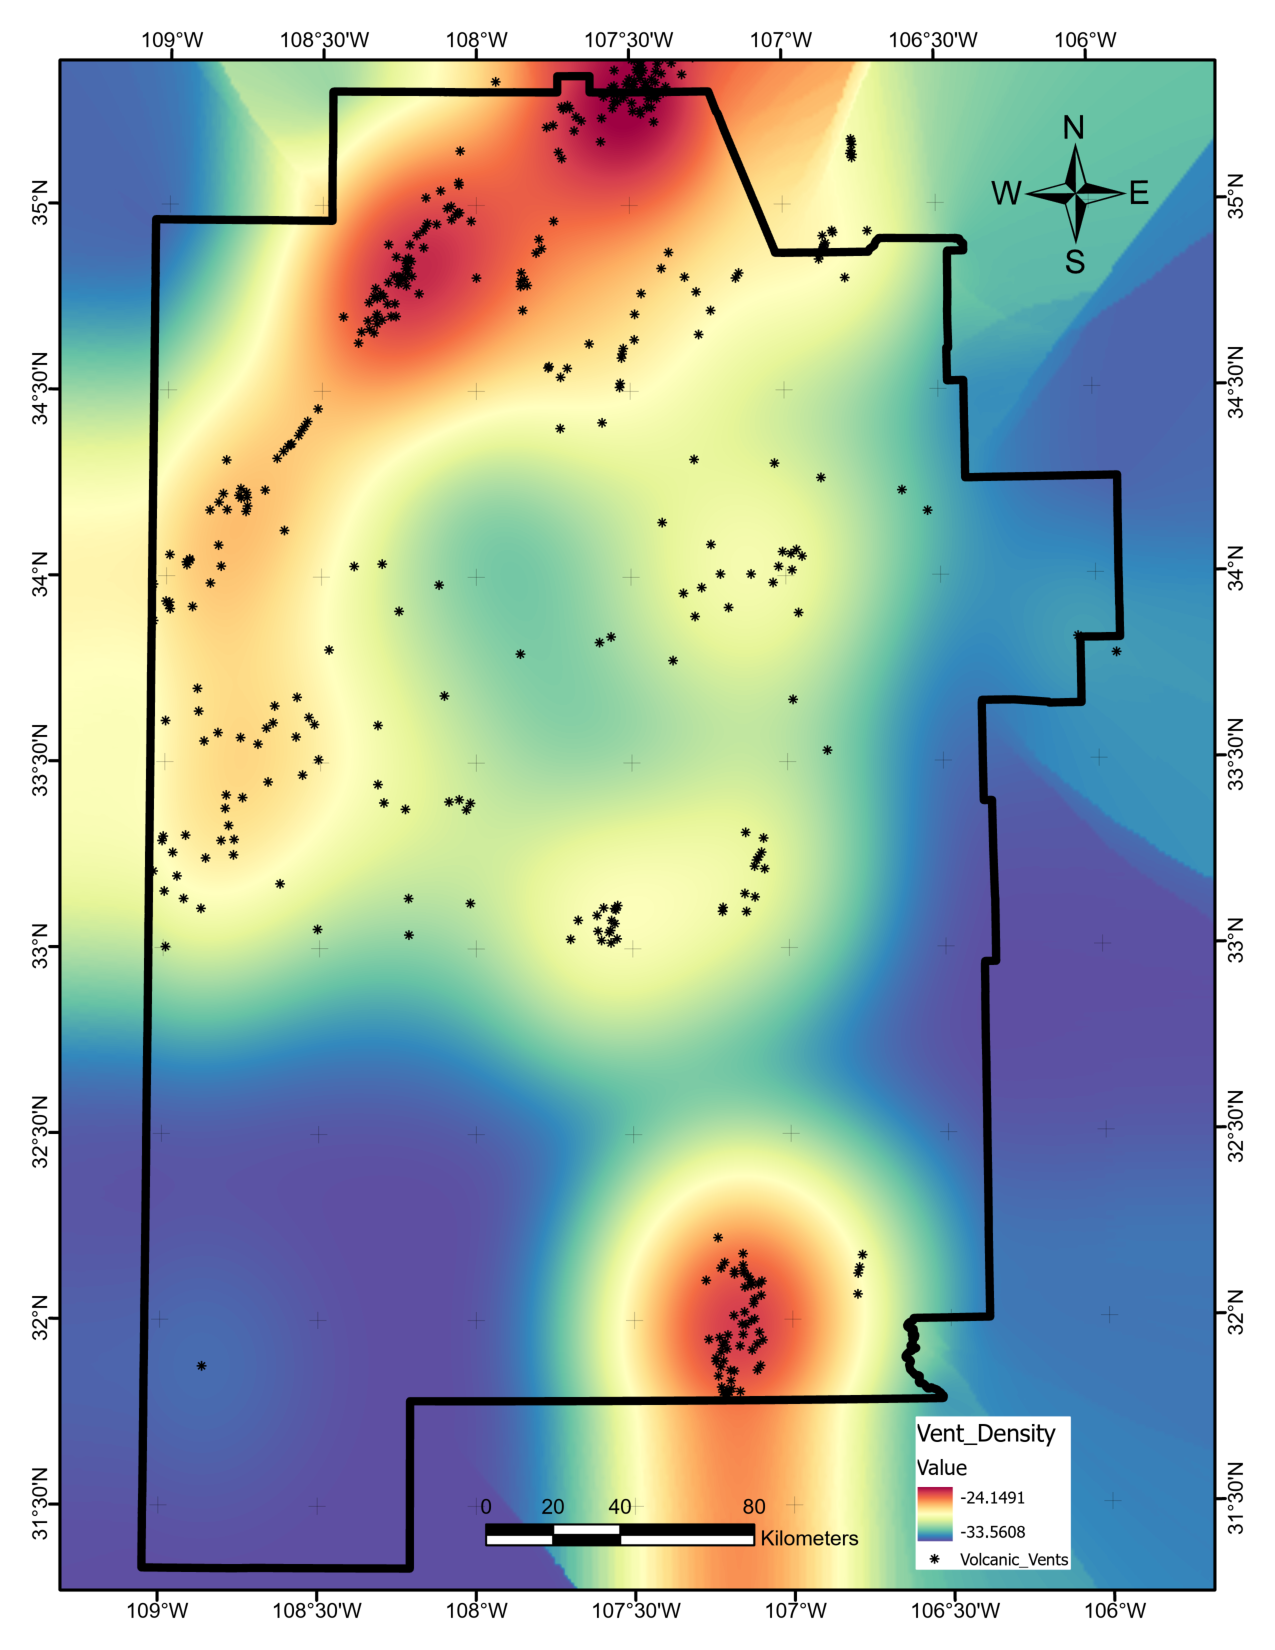
\includegraphics[scale=.50]{templates/images/Figure-VentDensity.pdf}
\caption[Volcanic vent data layer]{Volcanic vent density data layer. Units are in log(points/km$^2$). Black dots indicate vent locations from \protect\citep{nmbgmr_nmbgmr_2021}}
\label{fig:feat_vents}
\end{figure}

\subsubsection{Water Table Depth}

\citet{bielicki_hydrogeolgic_2015} mapped depth to the water table using data from the USGS and several additional sources. This raster was downloaded from their OpenEI submission \citep{kelley_geothermal_2015} and imported into ArcGIS. Data gaps between the raster extent and AOI polygon to the south and the east necessitated extrapolation of the layer, so ArcGIS \textit{Empirical Bayes Kriging} was applied to fill in the missing values. After some trial-and-error, the chosen parameter values for the final layer (Figure \ref{fig:feat_wtdepth}) included: output cell size of 0.01, empirical data transformation type, maximum of 100 points in each local model, 100 simulated exponential semivariograms, and a standard circular search neighborhood with a radius of 1.265 (auto-determined), minimum of 10 neighbors, and maximum of 15 neighbors.

\begin{figure}[!htp]
\centering
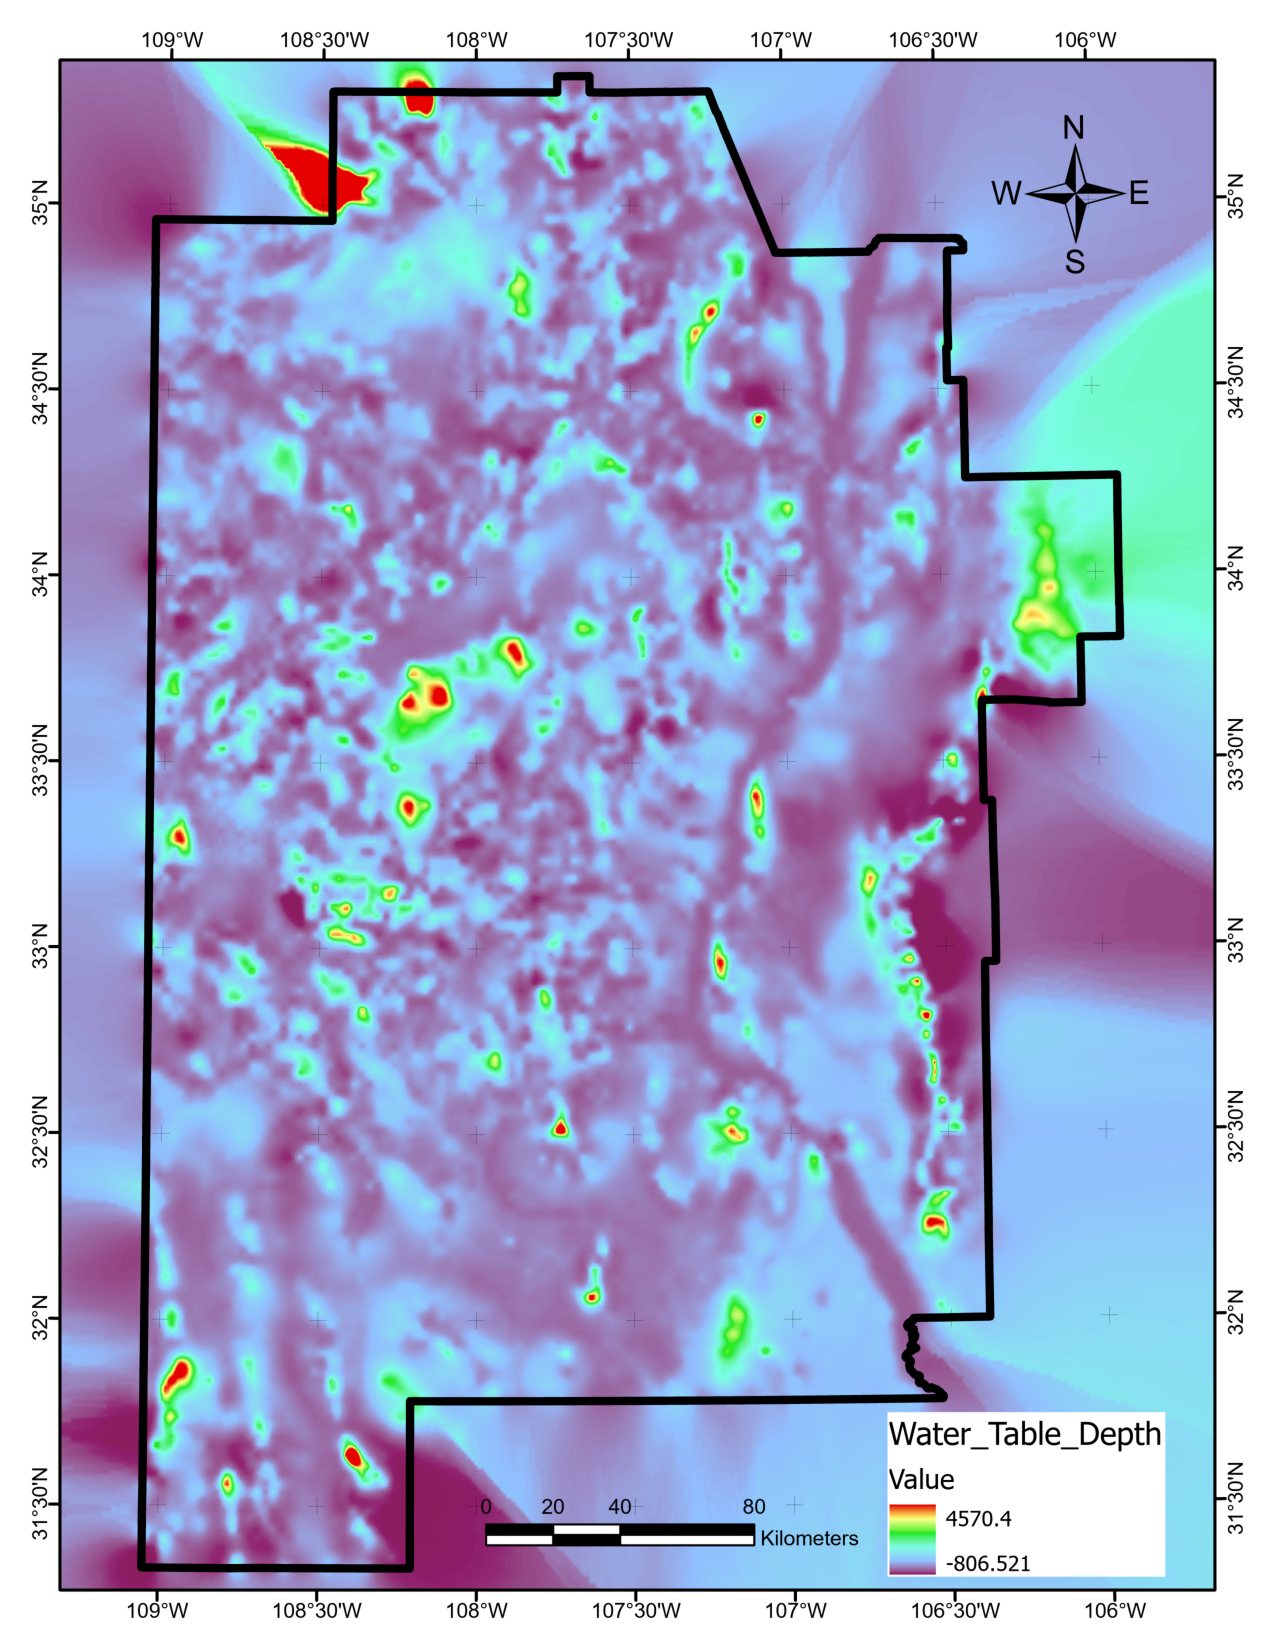
\includegraphics[scale=.50]{templates/images/Figure-WTDepth.pdf}
\caption[Water table depth data layer]{Water table depth data layer. Units are in feet. Adapted from raster created by \protect\citep{bielicki_hydrogeolgic_2015}.}
\label{fig:feat_wtdepth}
\end{figure}

\subsubsection{Water Table Gradient}

A pre-calculated grid for the water table gradient is among the layers included in the southwestern NM PFA archive \citep{kelley_geothermal_2015}. These data were downloaded and imported into ArcGIS. In order to fill data gaps between the raster extent and the AOI polygon to the south and the east, the ArcGIS \textit{Empirical Bayes Kriging} process was applied. After some trial-and-error, the final layer (Figure \ref{fig:feat_wt_gradient}) was generated using the following parameter values: output cell size of 0.01, empirical data transformation type, maximum of 100 points in each local model, 100 simulated exponential semivariograms, and a standard circular search neighborhood with a radius of 1.265 (auto-determined), minimum of 10 neighbors, and maximum of 15 neighbors.

\begin{figure}[!htp]
\centering
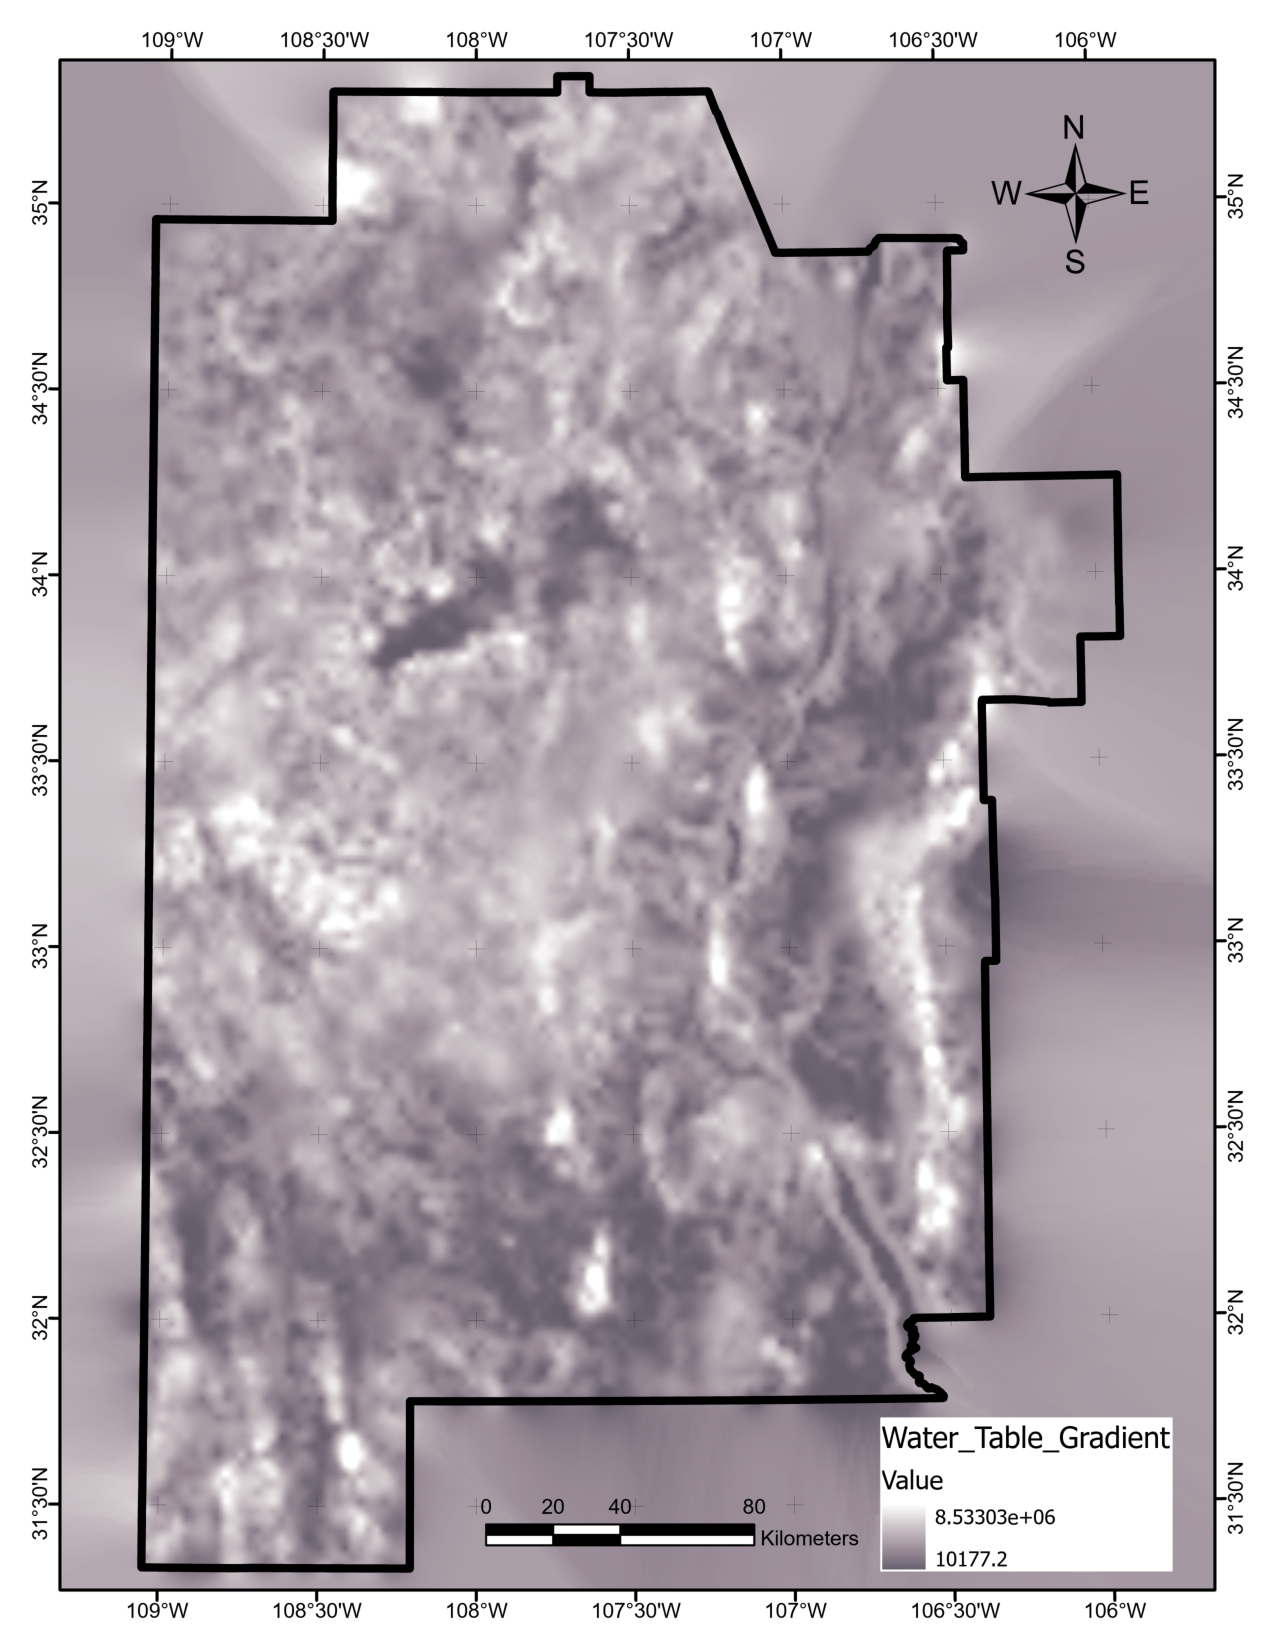
\includegraphics[scale=.50]{templates/images/Figure-WTGradient.pdf}
\caption[Water table gradient data layer]{Water table gradient data layer. Units are in feet/degrees. Based on raster from \protect\citep{bielicki_hydrogeolgic_2015}.}
\label{fig:feat_wt_gradient}
\end{figure}

\subsubsection{Geothermal Gradient}

The response variable for this analysis comes from observations stored in the SMU \textit{Heat Flow Database from \acrlong{bht} Data}, accessed via the SMU node of the \acrlong{ngds} (\acrshort{ngds}) \citep{smu_geothermal_2021}. This database focuses specifically on heat flow values calculated using geothermal gradient and conductivity measurements from well data in journal articles, books, reports, and from other sources \citep{blackwell_geothermal_2014}. Geothermal gradient values are provided in two forms: reported gradient and corrected gradient. The latter reports the result of both temperature and terrain corrections based on the well depth interval that a measurement was taken. If a corrected geothermal gradient value existed, this value was used in this analysis, otherwise the regular geothermal gradient value was selected. The well data set was clipped to the bounds of the Regional Polygon, then loaded into Python for conditioning. Well records missing geographic coordinates or a geothermal gradient value of either type were dropped. The list was sorted on coordinates and gradient, and only the first record for each location (well) was kept. The sort was in descending order, so this method preserved the highest gradient value captured per well. The final set of 599 values shown in Figure \ref{fig:feat_geotherm_gradient} comprise the raw input data used for predictive modeling of geothermal gradient across the study AOI.

\begin{figure}[!htp]
\centering
\includegraphics[scale=.50]{templates/images/Figure-GeothermalGrad_OrigWells.pdf}
\caption[Geothermal gradient data layer]{Geothermal gradient observations from well data. Units are in $^\circ$C/km. Data retrieved from the SMU NGDS portal \protect\citep{smu_geothermal_2021}}
\label{fig:feat_geotherm_gradient}
\end{figure}

A geothermal gradient layer also exists within the \citeauthor{bielicki_hydrogeolgic_2015} OpenEI submission \citep{kelley_geothermal_2015}, based primarily on a prior version of the SMU well data set. The layer nearly covers the full AOI, except for a missing section in the southernmost “toe” of the study area (Figure \ref{fig:feat_pfa_geotherm_gradient}A). Extrapolation was performed using the ArcGIS \textit{Empirical Bayes Kriging} function to create a complete map (Figure \ref{fig:feat_pfa_geotherm_gradient}B) using the following parameters: output cell size of 0.01, empirical data transformation type, a maximum of 100 points in each local model, 100 simulated semivariograms with exponential model type, and a standard circular search neighborhood with a radius of 1.265 (auto-determined), minimum of 10 neighbors, and maximum of 15 neighbors. This layer was saved as a reference map for later comparison with predictive model results.  

\begin{figure}[!htp]
\centering
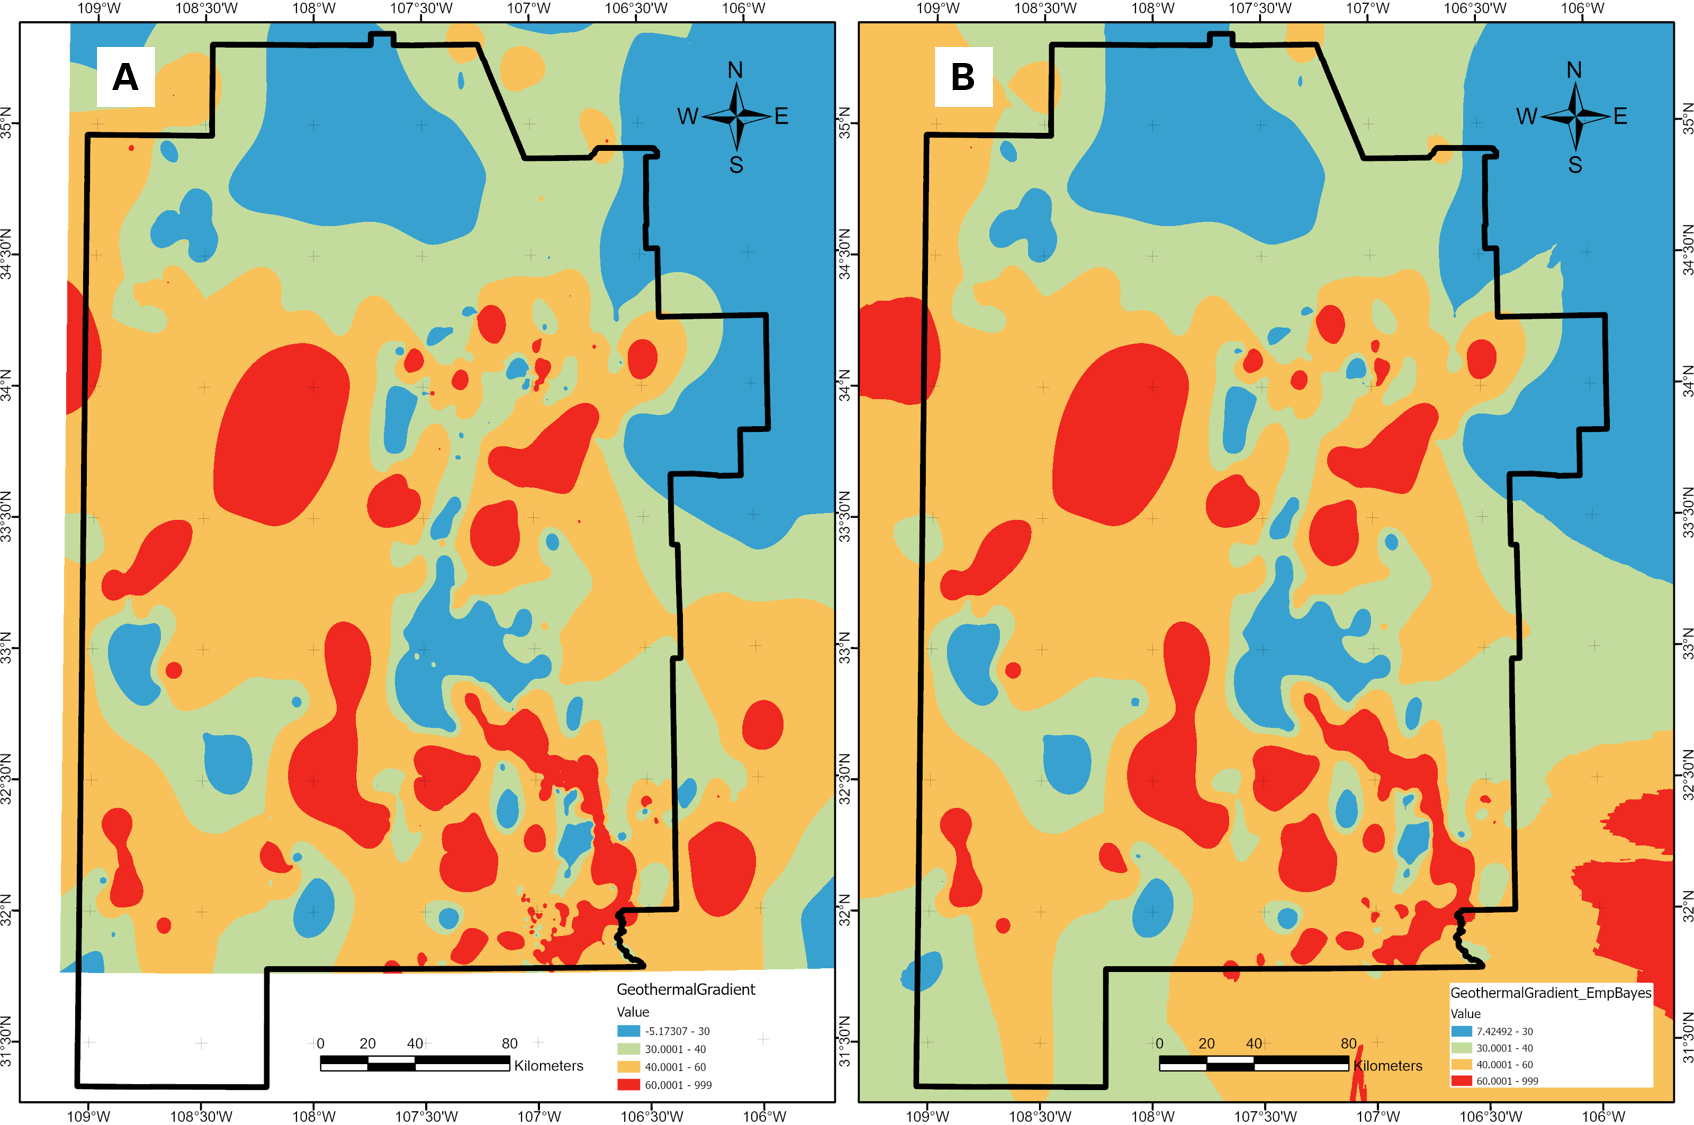
\includegraphics[scale=.50]{templates/images/Figure-PFA_Geothermal_Gradient_sidebyside.png}
\caption[Geothermal gradient data layer]{Geothermal gradient data layer. Units are in $^\circ$C/km. A. Raster originally created by \protect\citet{bielicki_hydrogeolgic_2015}. B. Extrapolation performed using ArcGIS \textit{Empirical Bayes Kriging} to fill in southern data gap.}
\label{fig:feat_pfa_geotherm_gradient}
\end{figure}

\subsection{Data Conditioning}\label{ch3:conditioning}
\begin{wrapfigure}{R}{0.35\linewidth}
\centering
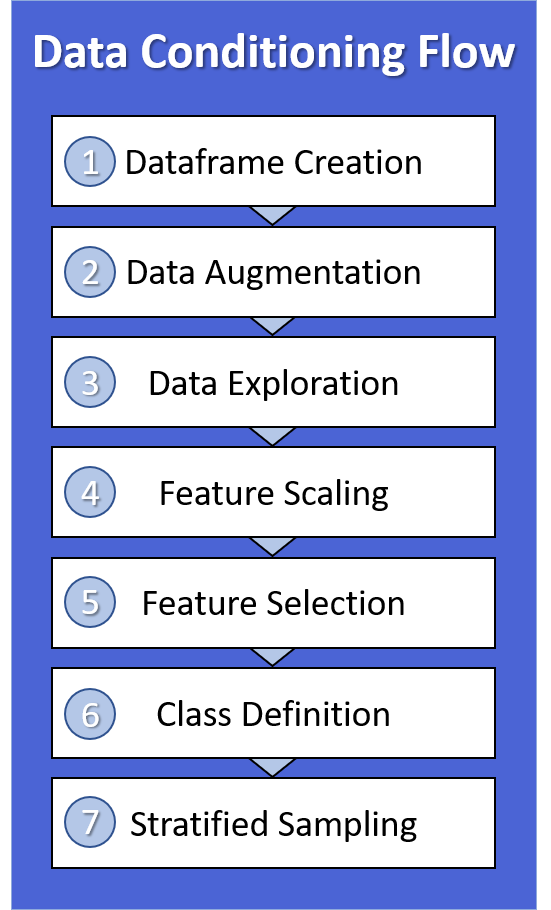
\includegraphics[scale=0.57]{templates/images/Flow-DataConditioning.png}
\singlespacing
\caption[Data conditioning workflow]{Workflow for conditioning data prior to predictive modeling.}
\label{fig:DC_Flow}
\end{wrapfigure}
After collecting the various data layers, several data conditioning steps were taken in order to explore variable relationships, rationalize feature selection, and prepare the data values for modeling. Figure \ref{fig:DC_Flow} outlines the general workflow followed, detailed more extensively below.

\subsubsection{Dataframe Creation}
Feature maps spanning the entire AOI provide the primary resource for creating a data set, but predictions of geothermal gradient require ground truth observations for training a predictive model. Initially, two separate data sets could be constructed for further evaluation. First, a full data set (FDS) consisting of a fishnet extraction of the feature values (Figure \ref{fig:fishnet}), which resulted in 15,137 records for the 25 predictors but no corresponding response variable values. The second was built from the actual geothermal gradient observations in the SMU data set, combined with 25 feature values extracted from the layer maps at the observation locations. This data set is hereafter referred to as the wells data set or WDS. Both FDS and WDS were stored in geodataframes consisting of the feature values and their associated latitude and longitude coordinates. These structured matrices are compatible with machine learning techniques like those found in the scikit-learn \citep{pedregosa_scikit-learn_2011} and TensorFlow \citep{abadi_tensorflow_2016} Python packages. 

\subsubsection{Data Augmentation}
\begin{wrapfigure}{R}{0.5\linewidth}
\centering
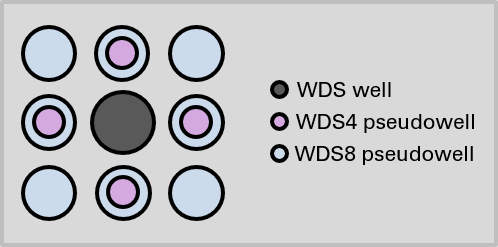
\includegraphics[scale=0.9]{templates/images/Figure-AugmentedWells.png}
\singlespacing
\caption[Data augmentation strategy]{Data augmentation strategy creates neighboring well locations around each original well in the WDS (dark gray). For WDS4, pseudowells (purple) are placed to the N, S, E, and W. For WDS8, pseudowells (blue) are placed at eight locations around the central well. Latitude and longitude offsets are $\pm0.01^\circ$ for pseudowell placement.}
\label{fig:data_augmentation}
\end{wrapfigure}

Noting that the AOI under investigation spans over 97,000 km$^2$, the relatively small size of the WDS raises concern over whether enough data is available to provide well-established data-driven insights using supervised learning methods. If predictions are reduced to just locations within the fishnet point set, there is still 2 orders of magnitude difference between ground truth observations and the points being predicted, exacerbated further by the need to partition the input data into one subset for training and two others for model validation and testing \citep[e.g.,][~p. 222]{hastie_elements_2009}. 

Data augmentation methods attempt to boost the size of a sparse input data set by using basic assumptions or heuristics to create additional input points. This study applies the concept of spatial autocorrelation at the heart of variography and kriging methods; in geography, all things are related, but the correlation increases as the spatial distance decreases \citep[~chap. 13]{gimond_intro_2021}. For each well location in the WDS, an additional four points were placed to the north, south, east, and west by adding or subtracting a constant 0.01$^\circ$ to each well’s geographic coordinates (Figure \ref{fig:data_augmentation}). Feature values were extracted from the layer maps in ArcGIS at these “pseudowell” locations. For the geothermal gradient, an interpolation layer was created using the ArcGIS \textit{Kriging} function with spherical variogram, auto-determined lag size of 0.097, and variable search radius with 12-point requirement. Gradient values were extracted from this layer for each pseudowell. The use of an interpolated gradient layer avoided conflict between pseudowells from close-proximity real well locations, where the direct assignment of the original well gradient values to step-out pseudowells would create an inconsistent augmented data set due to overlap. This overall workflow generated a new data set with 2,995 observations within the study AOI, referred to as WDS4. 

Extending this method further, a second augmented data set placed pseudowells to the NE, SE, NW, and SW as well, resulting in eight pseudowells for every original well in the WDS (Figure \ref{fig:data_augmentation}). Restricting the results to the AOI, this produced a data set with 5,386 observations (WDS8) for use in training and testing of machine learning models.

\subsubsection{Data Exploration}
The comprehensive coverage of the FDS makes it an appealing data set to use for exploring the attributes and relationships of the 25 data layers. Although care was taken to ensure each layer fully spanned the AOI, a search for missing values identified 163 \acrshort{nan}s (not a number, i.e., unassigned values) among the features. The corresponding rows plot along the study area boundary and likely represent places where one or more data layers ended just short of the fishnet point locations. These rows were dropped from the overall data set, reducing its size to 15,007 records.

Histograms offer insights into the data distribution for the predictor variables. Based on Figure \ref{fig:unscaled_hists}, only the magnetic anomaly layer has the appearance of a zero-mean Gaussian distribution. All other variables are offset and skewed to some extent. Many statistical tools rely on the assumption of normally-distributed random variables, so skewness can be problematic for modeling \citep[~p. 85]{montgomery_statistical_2012}.  These results suggest variable scaling and transformations will be a useful part of data preparation \citep[~p. 221]{montgomery_statistical_2012}. 

\begin{figure}[!htp]
\centering
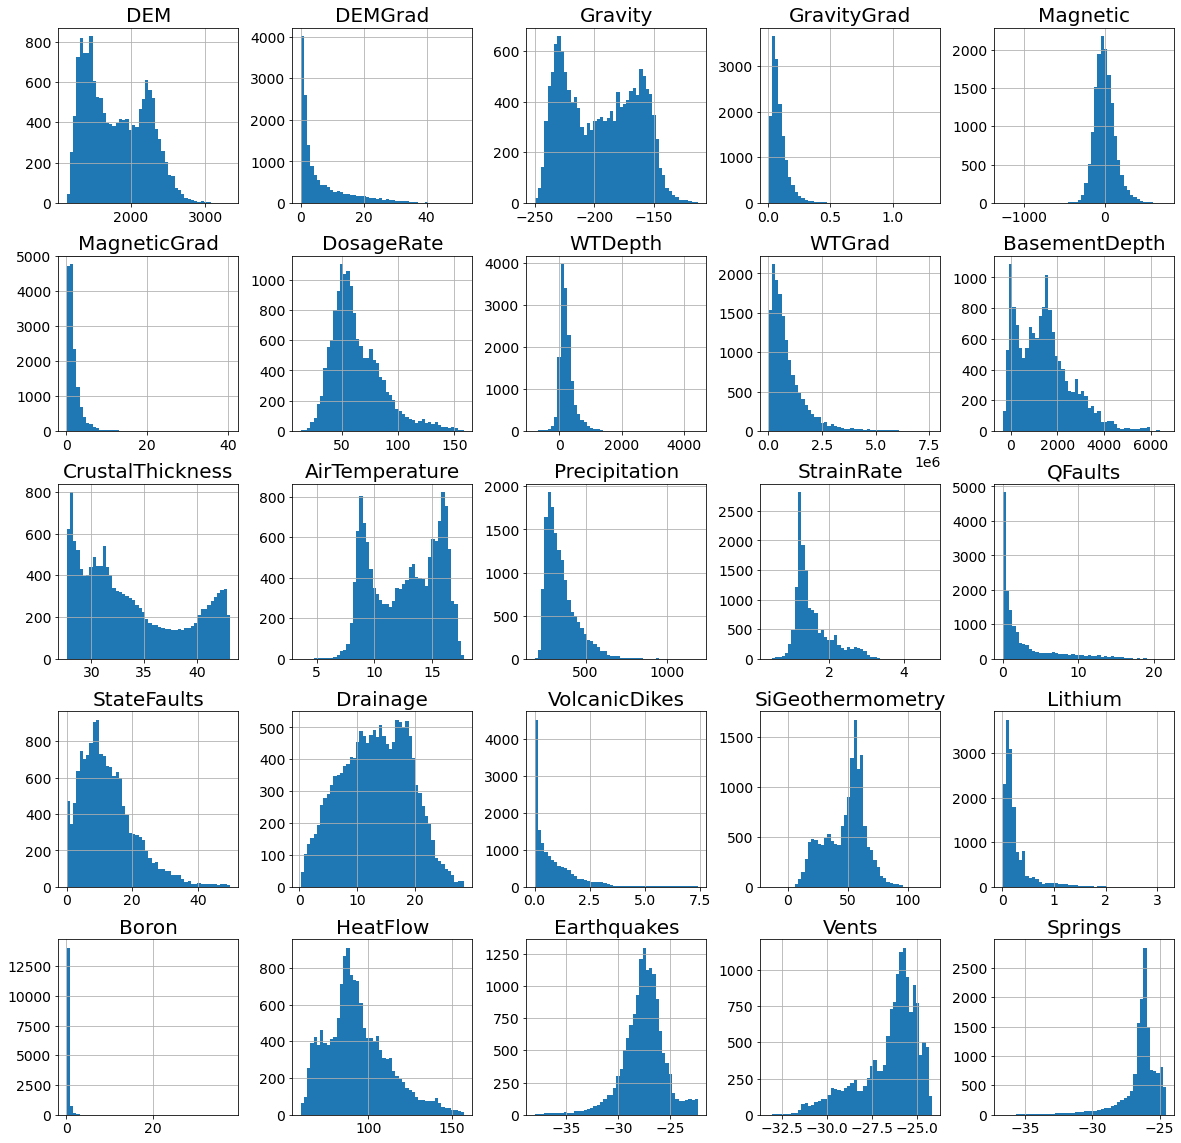
\includegraphics[width=\textwidth]{templates/images/Figure-Unscaled_Histograms.png}
\caption[Unscaled FDS histograms]{Histograms of the 25 features using 50 bins and the FDS. No scaling or transformations were applied to the data.}
\label{fig:unscaled_hists}
\end{figure}

Scatter plots between variables can highlight collinear behavior where a close relationship between two predictors creates uncertainty in their balance, that is, their individual contributions to the response variable \citep[~p. 99]{james_introduction_2013}. This can reduce the accuracy of model parameters like regression coefficients, impact the statistical significance of predictors, and lead to overly complex models \citep[~p. 100-101]{james_introduction_2013}. Figure \ref{fig:unscaled_scatter} illustrates all permutations of feature pairwise relationships. Although individual plots are too small to appreciate in detail, the overall shapes of the plots suggests some linear behavior between a handful of variables. The inset maps illustrate two examples of collinearity, and the third shows how skewness in variable distributions makes it difficult to discern some feature relationships.

\begin{figure}[!htp]
\centering
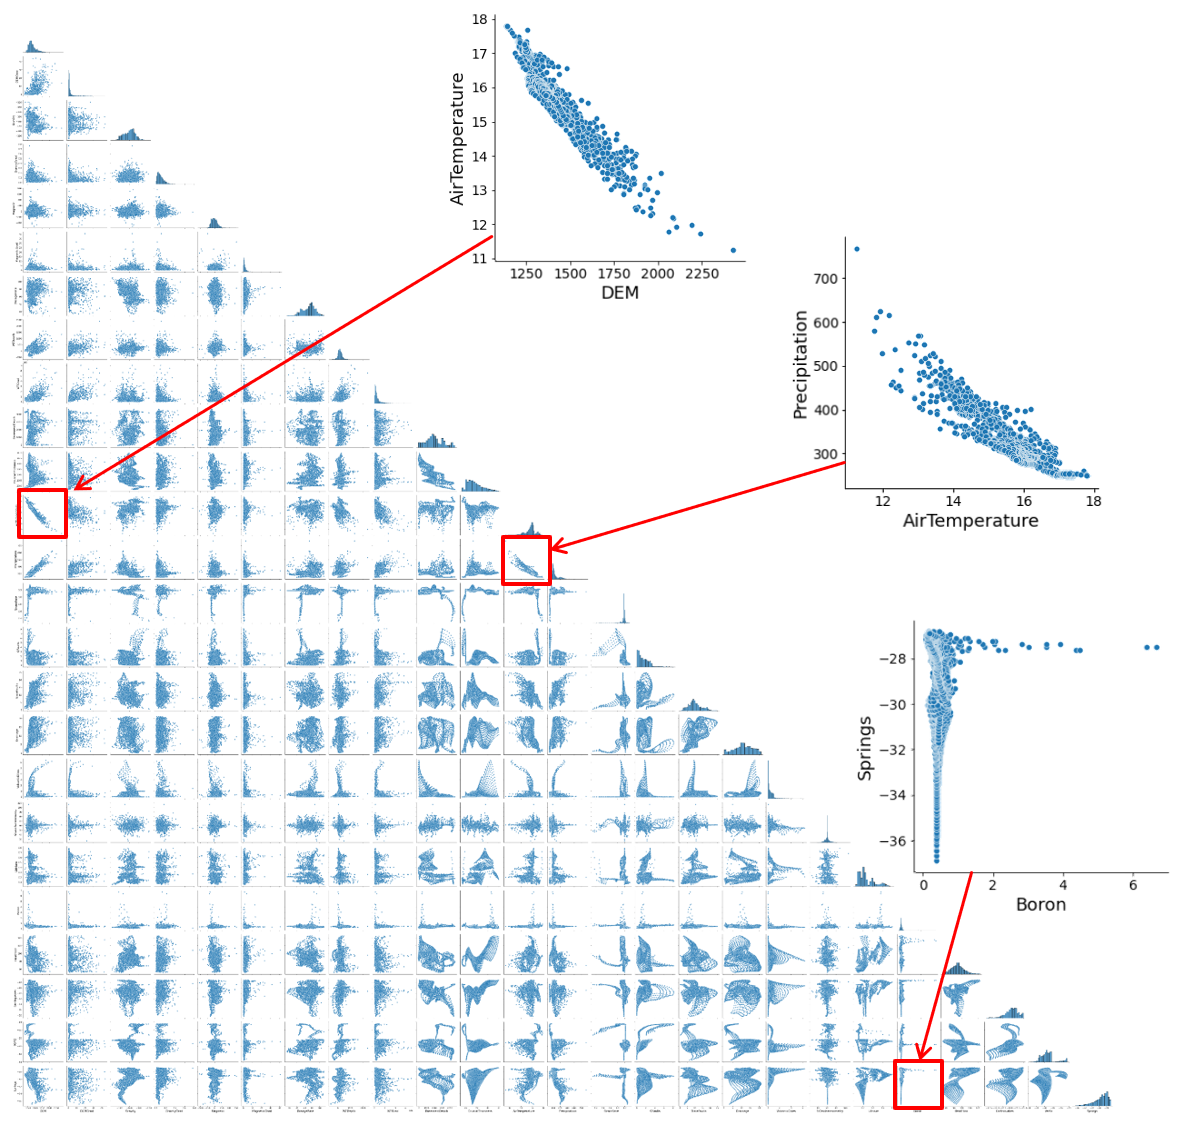
\includegraphics[width=\textwidth]{templates/images/Figure-Scatterplot_Unscaled_Features.png}
\caption[Unscaled FDS scatter plots]{Scatter plots between all possible pairs of the 25 features. The upper two plot call-outs illustrate collinear relationships. The lowermost highlighted plot shows the impact of skewed distributions. Note the difference in axis ranges depending on the variable. All plots show the first 2,000 points of the 15,007-point FDS.}
\label{fig:unscaled_scatter}
\end{figure}

\subsubsection{Feature Scaling}\label{ch3:scaling}
Large differences in the ranges and average values of the predictor variables are also evident in the scatter plots in Figure \ref{fig:unscaled_scatter}. For some machine learning algorithms, variables with larger value ranges can have an out-sized effect on the model, so scaling variables to comparable ranges and removing variable bias is an important step in data conditioning. Scaling also makes a predictor more standard Normal in appearance, i.e., $N(\mu=0, \sigma=1)$, as implicitly required by some statistical methods. The scikit-learn \textit{StandardScalar} function transforms data using the Z-score formulation \citep{scikit-learn_sklearnpreprocessingstandardscaler_2021}:

\begin{equation}
    Z = \frac{(x - \mu)}{\sigma}
\end{equation}

This data scaling can be directly paired with non-linear data transformations that alter the shape of variable distributions, replacing skewness with more Gaussian-like symmetry. One such transformation is the Yeo-Johnson method, which can handle both positive and negative data. The Yeo-Johnson power transformation actually represents a family of transformations, the choice of which depends on a hyperparameter $\lambda$ \citep{yeo_new_2000}:

\begin{equation}
    x_i^{(\lambda)} = 
    \begin{cases}
      [(x_i + 1)^{\lambda)}-1]/\lambda & \text{if $\lambda \neq 0$, $x_i \geq 0$,}\\
      \ln{(x_i + 1)} & \text{if $\lambda = 0$, $x_i \geq 0$,}\\
      -[(-x_i + 1)^{2-\lambda}-1]/(2-\lambda) & \text{if $\lambda \neq 2$, $x_i < 0$,}\\
      -\ln{(-x_i + 1)} & \text{if $\lambda = 2$, $x_i < 0$}
    \end{cases}  
\end{equation}

Scikit-learn supports Yeo-Johnson through the \textit{PowerTransformer} preprocessing tool that automatically estimates the $\lambda$ parameter using maximum likelihood \citep{scikit-learn_sklearnpreprocessingpowertransformer_2021}. Figure \ref{fig:scaled_hist} shows the same histograms after applying both standard scaling and Yeo-Johnson transformation to the predictor variables. Many of the distributions appear much less skewed, and all have zero-mean and unit variance.

\begin{figure}[!htp]
\centering
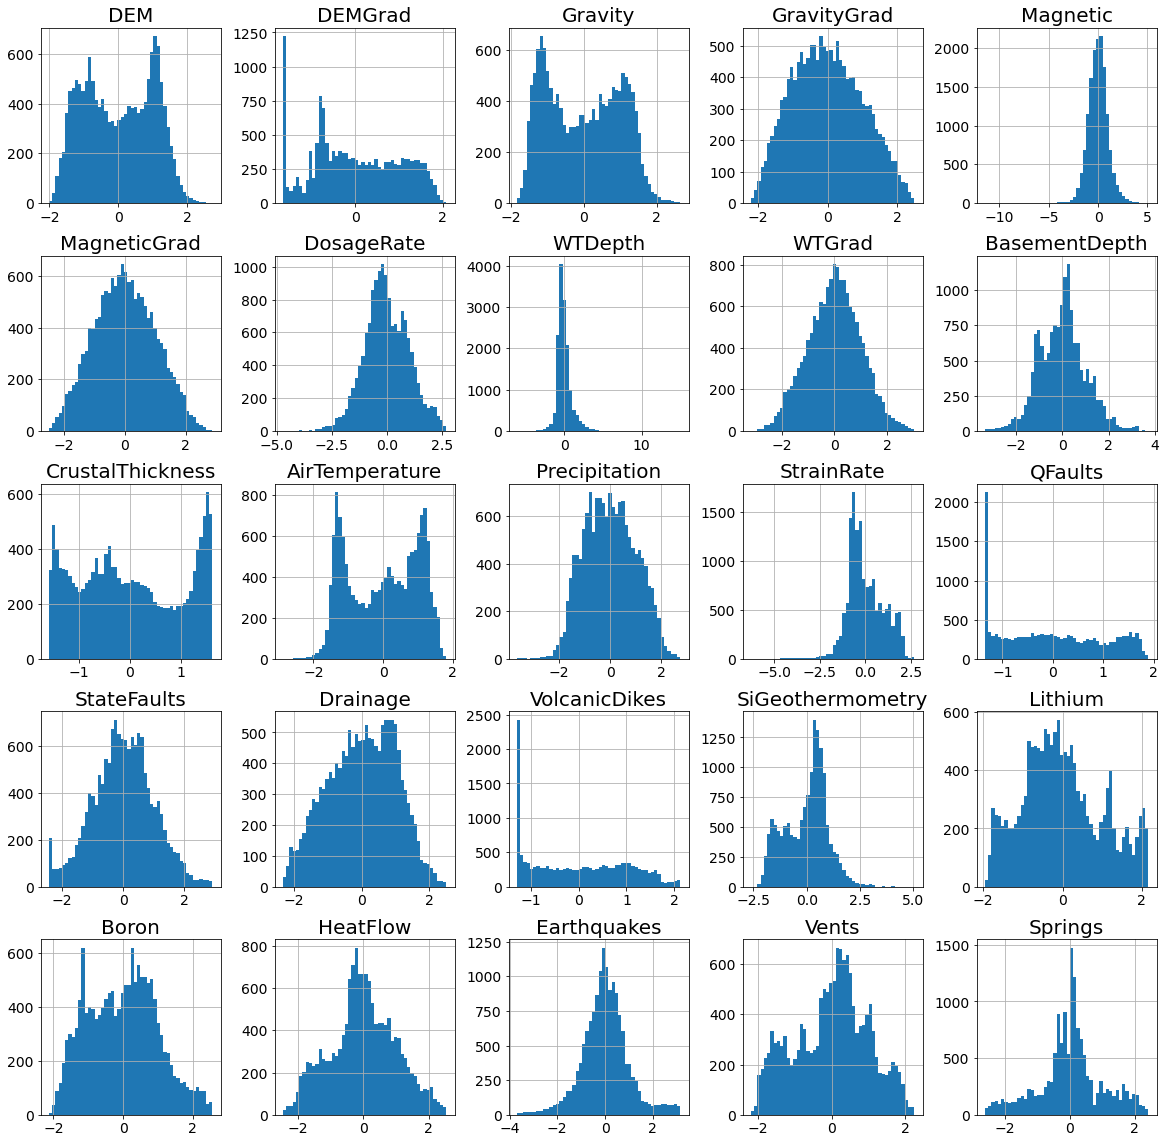
\includegraphics[width=\textwidth]{templates/images/Figure-Scaled_Histograms.png}
\caption[Scaled FDS histograms]{Histograms of the 25 features after standard scaling and Yeo-Johnson transformation of the FDS. Plots use 50 bins.}
\label{fig:scaled_hist}
\end{figure}

Scaling and transformation also impacts the variable pairwise scatter plots. Figure \ref{fig:scaled_scatter} illustrates the improvement in scatter plot appearances as a result of the feature conditioning. With greater spread in the variable distributions, relationships are more readily apparent.

\begin{figure}[!htp]
\centering
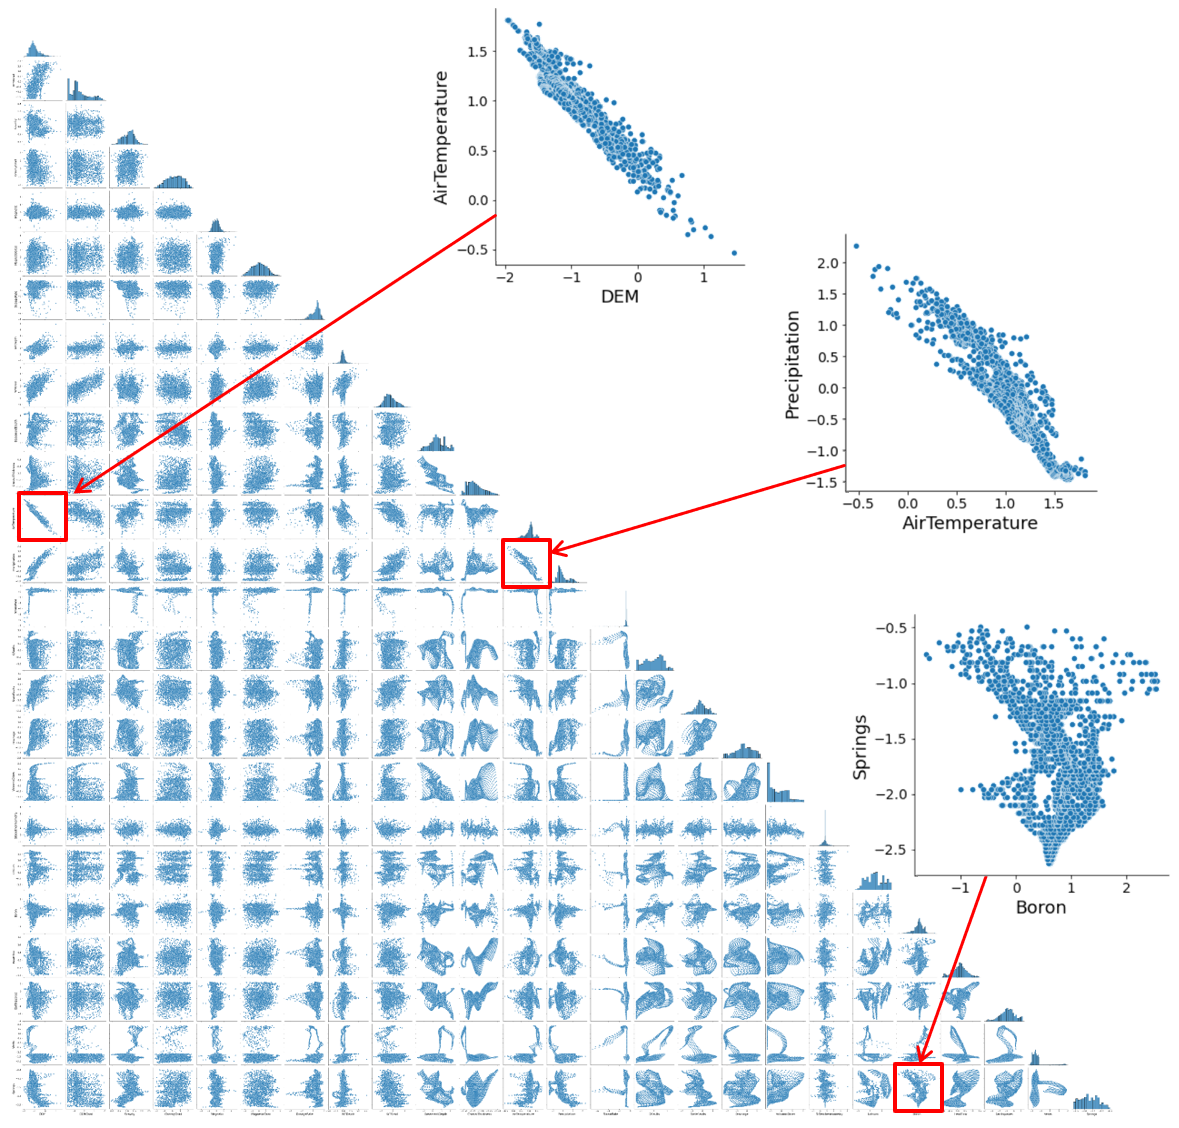
\includegraphics[width=\textwidth]{templates/images/Figure-Scatterplot_Scaled_Features.png}
\caption[Scaled FDS scatter plots]{Scatter plots between all possible pairs of the 25 features after standard scaling and Yeo-Johnson transformation of the FDS. The upper two plot call-outs illustrate collinear relationships. The lowermost highlighted plot shows the impact of Yeo-Johnson transformation on revealing variable relationships that were hidden by skewed distributions. All plots show the first 2,000 points of the 15,007-point FDS.}
\label{fig:scaled_scatter}
\end{figure}

\subsubsection{Feature Correlation}\label{ch3:feat_corr}
Another way to evaluate collinearity between two features is to calculate their correlation coefficient. The standard Pearson correlation coefficient ($r$) is strictly defined as the covariance between two variables, scaled by the product of their standard deviations. On a per-sample basis, this becomes \citep[~p. 70]{james_introduction_2013}:

\begin{equation}
    r = \frac{\Sigma(x_i-\bar{x})(y_i-\bar{y})}{\sqrt{\Sigma{(x_i-\bar{x})^2} \Sigma{(y_i-\bar{y})^2}}}
\end{equation}

When $r$ is close to zero, no measurable covariance takes place between the two variables. Values close to 1 or -1 suggest the two variables are linearly-related, where the sign indicates direction of the relationship. A lower triangular matrix of pairwise correlation coefficients was calculated using the scaled, transformed version of FDS (Figure \ref{fig:corr_matrix}). Average Air Temperature stands out as highly collinear with multiple variables: DEM (-0.97), Gravity Anomaly (0.89), and Crustal Thickness (-0.89). Crustal Thickness also shows some collinearity with Gravity Anomaly (-0.88) and DEM (0.80). The same is true for Gravity and DEM (-0.83).

\begin{figure}[!htp]
\centering
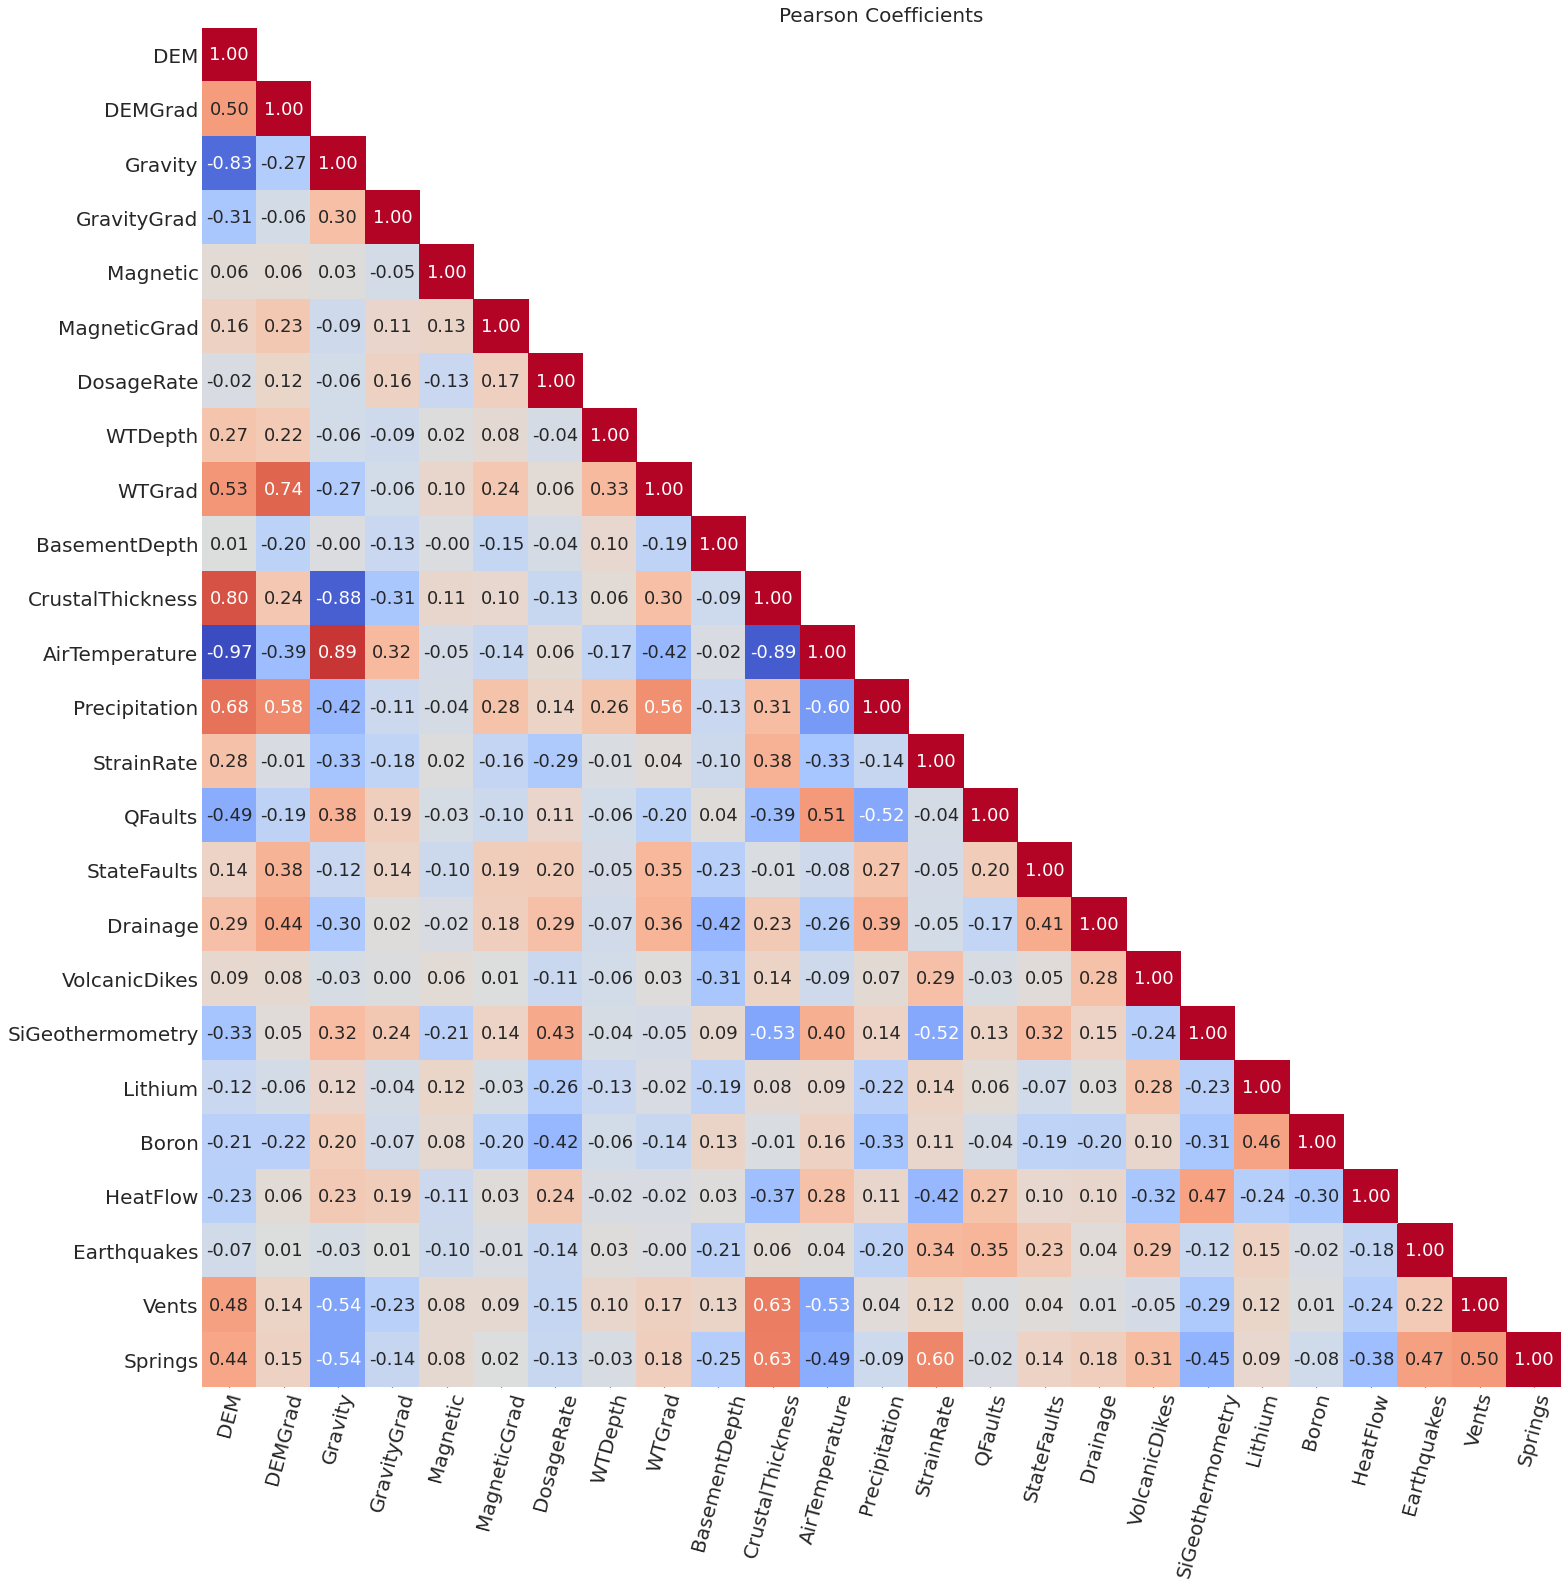
\includegraphics[width=\textwidth]{templates/images/Figure-Scaled_Correlation_Matrix.png}
\caption[Feature correlation matrix]{Correlation matrix with Pearson correlation scores for each feature pair based on the scaled and transformed version of the FDS.}
\label{fig:corr_matrix}
\end{figure}

Focusing on the related Earth systems, the logic behind these relationships makes sense. High surface elevations recorded in the DEM layer will have correspondingly lower average air temperatures -- hence snow caps appearing on mountains. In addition, if the crust is assumed to be in isostatic equilibrium with the mantle like an iceberg floating in the ocean, topographic highs will be supported by thick roots and DEM will directly covary with crustal thickness. And since crustal densities are less than those of the underlying mantle, displacement of upper mantle by crustal roots (high crustal thickness) results in a lower average density and negative gravity anomaly values. The reverse is true as well; thinner crust will correspondingly tie to positive gravity anomaly values.  

Of these variables, only Air Temperature and DEM have a correlation value over 0.9. In fact, a 0.97 $r$-value suggests Air Temperature and DEM are nearly interchangeable in the value of information they provide to a predictive model. Since air temperature does not directly relate to subsurface characteristics except for the thermal conditions at zero-depth, Average Air Temperature can be removed from the main set of predictors to reduce overall collinearity in the data set. Crustal Thickness and Gravity Anomaly both similarly show non-ideal $r$-values, but feature ranking while modeling will provide another opportunity to consider which of them might need to be dropped.

\subsubsection{Classification Options}

Geothermal gradient can be treated as a continuous variable and predicted directly using regression methods. Alternatively, binning the geothermal gradient into discrete ranges changes the approach into a classification problem. In the context of exploration, geospatial classifications have a direct corollary in PFA favorability mapping and other simplified displays of complex risk. Furthermore, regression model results provide exact geothermal gradient estimates, which could be easily mistaken for certainty in a largely under-constrained problem. The binning approach is adopted in this thesis, largely based on the work of previous researchers.

\begin{wraptable}{R}{0.4\linewidth}
\centering
\begin{tabular}{|c|c|}
\hline
\textbf{Gradient Range} & \textbf{Class} \\ \hline
{[}\;0$^\circ$C/km, 30$^\circ$C/km)     & 0                    \\ \hline
{[}\;30$^\circ$C/km, 40$^\circ$C/km)    & 1                    \\ \hline
{[}\;40$^\circ$C/km, 60$^\circ$C/km)    & 2                    \\ \hline
{[}\;60$^\circ$C/km, 999$^\circ$C/km)   & 3                    \\ \hline
\end{tabular}
\singlespacing
\caption[Geothermal gradient classes]{Geothermal gradient ranges and assigned class values. Ranges are left-inclusive.}
\label{tab:geothermal_gradient_classes}
\end{wraptable}

The \textit{Geothermal Gradient Map of the Conterminous United States} published in 1991 separates geothermal gradient into five 15 $^\circ$C/km bins that end with 60-75+ $^\circ$C/km \citep{lanl_geothermal_1991}. \citet{armstead_heat_1987} instead defined non-thermal gradients as 20-25 $^\circ$C/km, thermal gradients as $\leq$38 $^\circ$C/km, and hydrothermal gradients as 60-80 $^\circ$C/km on average. \citet{tester_economic_1990} reframed this model with representative values for three EGS grades: high = 80 $^\circ$C/km, mid = 50 $^\circ$C/km, and low = 30 $^\circ$C/km. In a later iteration, \citet{herzog_economic_1997} reasserted ranges for EGS resources: high-grade for >60 $^\circ$C/km, mid-grade for 40-60 $^\circ$C/km, and low-grade for <40 $^\circ$C/km. This thesis extends the Herzog model by adding a non-thermal range as <30 $^\circ$C/km, recognizing the average geothermal gradient ranges from 25-30 $^\circ$C/km and anything below that would be ill-suited for geothermal exploration and development (Table \ref{tab:geothermal_gradient_classes}).

Preparation of well data sets WDS, WDS4, and WDS8 first involved removing records with NaN values or negative geothermal gradients. The remaining records were split into the gradient categories in Table \ref{tab:geothermal_gradient_classes}. Distributions of class values for all data sets are shown in Table \ref{tab:data_set_class_count}. For FDS, the class break-down is based on the extrapolated \citet{bielicki_hydrogeolgic_2015} geothermal gradient layer (Figure \ref{fig:feat_pfa_geotherm_gradient}) sampled using the point fishnet (Figure \ref{fig:fishnet}). Note that class imbalance exists in all data sets; mid-grade values dominate in the FDS, but the well data sets show a bias toward high-grade examples with few non-thermal examples. This is a common conundrum when using well data for characterization and analysis; drilling campaigns tend to target areas to drill based on chance of success rather than drilling at random, so low-side under-representation tends to be ubiquitous. The topic of class imbalance is discussed again in \textbf{Section XX}.  

\begin{table}[htp]
\centering
\begin{tabular}{c|c|c|c|c|}
\cline{2-5}
                              & FDS    & WDS & WDS4  & WDS8  \\ \hline
\multicolumn{1}{|c|}{Class 0} & 2,394  & 20  & 101   & 184   \\ \hline
\multicolumn{1}{|c|}{Class 1} & 4,432  & 99  & 499   & 905   \\ \hline
\multicolumn{1}{|c|}{Class 2} & 6,243  & 232 & 1,144 & 2029  \\ \hline
\multicolumn{1}{|c|}{Class 3} & 1,938  & 245 & 1,229 & 2226  \\ \hline
\multicolumn{1}{|c|}{Total}   & 15,007 & 596 & 2,973 & 5,344 \\ \hline
\end{tabular}
\caption[Data set class distribution]{Distribution of geothermal gradient classes for each data set.}
\label{tab:data_set_class_count}
\end{table}

\subsubsection{Stratified Sampling}

Supervised machine learning models determine the attributes of a predictive model based on the input data provided during training. In approximating the target function, i.e., the response variable, the models seek to minimize an objective function as much as possible. The pitfall here lies in the representativeness of the training data set; if a model exactly matches the input data, it may not generalize well to other unseen observations. This would be a high variance model, meaning the model predictions are strongly coupled to the characteristics of the training data. Variance trades off with model bias, which includes simplifying assumptions on the form of the target function. The bias-variance trade-off is a core concept in machine learning \citep[~p. 33-36]{james_introduction_2013} and drives many of the model decisions made within this thesis.

One method of reining in the high variance overfitting problem involves splitting the input data set into training and testing subsets. Model fitting uses the training set, while model evaluation relies on the test set. An additional split of the testing subset into separate validation and testing sets allows a modeler to validate model parameter choices with validation data not seen during model training, but then conduct a final model evaluation using completely unseen test data \citep[~p. 222]{hastie_elements_2009}. Creating such firm boundaries between seen and unseen data helps prevent the issue of data leakage.  Fundamentally, if a model trains or is tuned on data used to evaluate its performance, that evaluation no long reflects real world predictive ability because information from the evaluation data has already “leaked” into the model \citep{kaufman_leakage_2012}. When data leakage occurs, model performance after deployment will likely not match that seen during testing. In other words, it won’t be as good a model as the modeler thinks it is.

For classification problems, randomly splitting input data set into 3 subsets will violate the balance between class proportions in the original input data. Fortunately, sampling techniques exist that preserve the relative fractions of each class in the derivative subsets. Scikit-learn provides the \textit{StratifiedShuffleSplit} method for randomly sampling from each class subgroup to generate training, validation, and test sets that look like one another and the original complete data set \citep{scikit-learn_sklearnmodel_selectionstratifiedshufflesplit_2021}. The FDS, WDS, WDS4, and WDS8 data sets were each partitioned into 70\% training, 15\% validation, 15\% testing using this method. Table \ref{tab:stratified_split_counts} lists raw counts of observations associated with each class bucket and describes how class proportions compare across the different data sets.

Data leakage can be a concern when scaling or transforming split data sets. For example, the mean and standard deviation used for z-score normalization should be derived from the training subset before being applied to the validation and testing subsets. This maintains separability between seen and unseen data. For this reason, the train-validate-test splits of the four different data sets listed in Table \ref{tab:stratified_split_counts} were performed using the unscaled, untransformed versions of those data sets, and the feature scaling and Yeo-Johnson transformation discussed in Section \ref{ch3:scaling} are applied immediately before predictive modeling in a multi-step pipeline approach as discussed in Chapter \ref{ch5:expl_applied}.

\begin{table}[!htp]
\resizebox{\textwidth}{!}{
    \begin{tabular}{l|c|c|c|c|c|c|c|c|c|c|}
    \cline{2-11}
    \multicolumn{1}{c|}{} &
      \% &
      \begin{tabular}[c]{@{}c@{}}WDS\\ train\end{tabular} &
      \begin{tabular}[c]{@{}c@{}}WDS\\ validate\end{tabular} &
      \begin{tabular}[c]{@{}c@{}}WDS\\ test\end{tabular} &
      \begin{tabular}[c]{@{}c@{}}WDS4\\ train\end{tabular} &
      \begin{tabular}[c]{@{}c@{}}WDS4\\ validate\end{tabular} &
      \begin{tabular}[c]{@{}c@{}}WDS4\\ test\end{tabular} &
      \begin{tabular}[c]{@{}c@{}}WDS8\\ train\end{tabular} &
      \begin{tabular}[c]{@{}c@{}}WDS8\\ validate\end{tabular} &
      \begin{tabular}[c]{@{}c@{}}WDS8\\ test\end{tabular} \\ \hline
    \multicolumn{1}{|l|}{Class 0} & 3 & 14 & 3 & 3 & 71 & 15 & 15 & 129 & 27 & 28  \\ \hline
    \multicolumn{1}{|l|}{Class 1} & 17 & 69 & 15 & 15 & 349 & 75 & 75 & 633 & 136 & 136 \\ \hline
    \multicolumn{1}{|l|}{Class 2} & 38 & 162 & 35 & 35 & 801 & 171 & 172 & 1420 & 305 & 304 \\ \hline
    \multicolumn{1}{|l|}{Class 3} & 42 & 172 & 36 & 37 & 860 & 185 & 184 & 1558 & 334 & 334 \\ \hline
    \multicolumn{1}{|l|}{Total}   & 100 & 417 & 89 & 90 & 2,081 & 446 & 446 & 3,740 & 802 & 802 \\ \hline
    \end{tabular}}
\caption[Class count for test-train-validate split]{Raw observation counts for each geothermal gradient class across the different data sets after splitting each into training, validation, and testing subsets.}
\label{tab:stratified_split_counts}
\end{table}